%\documentclass[../../tesis.tex]{subfiles}
\documentclass[class=article, crop=false]{standalone}
\usepackage[subpreambles=true]{standalone}
\usepackage{import}
\graphicspath{{images/}}

\usepackage{longtable}
%

\usepackage{amssymb}
\usepackage{amsmath}
%\usepackage{natbib}
\setcounter{tocdepth}{3}
\usepackage{graphicx}
%\graphicspath{ {Graficos/} }
\usepackage{subfigure}
\usepackage{gensymb}
\usepackage{authblk}
\usepackage{url}
\usepackage[utf8]{inputenc}

\usepackage[spanish]{babel}
\selectlanguage{spanish}
%\usepackage[style=authoryear]{biblatex}


\begin{document}

La nomenclatura de Cadenas y Subcadenas utilizada en el presente trabajo proviene de \cite{molinari2016especializacion}. A su vez la clasificación en Usos proviene de \cite{flores2008world}
	
\subsection{Tabla de referencia: Descripción cadenas}



\begin{table}[!ht]
	\begin{tabular}{ll}
		\textbf{Cadena} & \textbf{Descripción} \\
		Agroind & Agroindustria \\
		Animal & Manufacturas De Origen Animal \\
		Automotriz & Automotriz \\
		Bebidas & Bebidas \\
		Bk & Bienes De Capital \\
		Combyene & Combustibles Y Energía \\
		Cuero & Marroquinería, Calzado Y Otras Manufacturas De Cuero Y Pieles \\
		Foreind & Foresto-Industria \\
		Insdif & Insumos Difundidos \\
		Medic & Medicamentos \\
		Oeqtransp & Otro Equipo De Transporte \\
		Texteind & Textil E Indumentaria \\
		Omanuf & Otras Manufacturas \\
		Oquim & Otros Químicos
	\end{tabular}
\caption{Descripción Cadenas}
\label{table:cadenas}
\end{table}



\subsection{Tabla de referencia: Descripción subcadenas}


% Please add the following required packages to your document preamble:
% \usepackage{longtable}
% Note: It may be necessary to compile the document several times to get a multi-page table to line up properly
\begin{longtable}[!ht]{lll}
	\caption{Descripción subcadenas}
	\label{tabla:subcadenas}
	\endlastfoot
	
	\textbf{Cadena} & \textbf{Subcadena} & \textbf{Descripción} \\
	\endhead
	%
	Agroindustria & Agroquim & Agroquímicos \\
	Agroindustria & Alimanim & Alimentos Para Animales \\
	Agroindustria & Ceryoleag & Cereales Y Oleaginosas \\
	Agroindustria & Flh & Frutas, Legumbres Y Hortalizas \\
	Agroindustria & Oagroind & Otros Agroindustria \\
	Animal & Aviar & Aviar \\
	Animal & Lácteos & Lácteos \\
	Animal & Oanimal & Otros Cadena Animal \\
	Animal & Pescado & Pescado \\
	Animal & Porcina & Porcina \\
	Animal & Vacuna & Vacuna \\
	Automotriz & Autopartes & Autopartes \\
	Automotriz & Autos & Autos \\
	Automotriz & Camyomnib & Camiones Y Ómnibus \\
	Automotriz & Oautom & Otros Automotriz \\
	Bebidas & Alcohol & Alcohólicas \\
	Bebidas & Noalco & No Alcohólicas \\
	Bebidas & Vino & Vino \\
	Bienes De Capital & Eqelec & Equipos Eléctricos \\
	Bienes De Capital & Eqmedico & Equpamiento Médico \\
	Bienes De Capital & Maqagr & Maquinaria Agrícola \\
	Bienes De Capital & Maqalim & Maquinaria Para Alimentos \\
	Bienes De Capital & Maqcomb & Maquinaria Para Combustibles \\
	Bienes De Capital & Maqfor & Maquinaria Forestal \\
	Bienes De Capital & Maqmet & Maquinaria Para Metales \\
	Bienes De Capital & Maqtextycuero & Maquinaria Para Textiles Y Cuero \\
	Bienes De Capital & Obk & Otros Bienes De Capital \\
	Bienes De Capital & Oeqtrans & Otro Equipo De Transporte \\
	Bienes De Capital & Vehyautop & Vehículos Y Autopartes \\
	Combustibles Y Energía & Biocomb & Biocombustibles \\
	Combustibles Y Energía & Electricidad & Electricidad \\
	Combustibles Y Energía & Gas & Gas \\
	Combustibles Y Energía & Nuclear & Nuclear \\
	Combustibles Y Energía & Ocombyene & Otros Combustibles Y Energía \\
	Combustibles Y Energía & Petroleo & Petróleo \\
	Combustibles Y Energía & Quimicos & Químicos \\
	\begin{tabular}[c]{@{}l@{}}Marroquinería, Calzado Y Otras\\ Manufacturas De Cuero Y Pieles\end{tabular} & Calzado & Calzado \\
	\begin{tabular}[c]{@{}l@{}}Marroquinería, Calzado Y Otras\\ Manufacturas De Cuero Y Pieles\end{tabular} & Cueros & Cueros \\
	\begin{tabular}[c]{@{}l@{}}Marroquinería, Calzado Y Otras\\ Manufacturas De Cuero Y Pieles\end{tabular} & Ocuero & Otros Cueros \\
	\begin{tabular}[c]{@{}l@{}}Marroquinería, Calzado Y Otras\\ Manufacturas De Cuero Y Pieles\end{tabular} & Quimcuero & Químicos Para Cueros \\
	Foresto-Industria & Grafica & Gráfica \\
	Foresto-Industria & Madymueb & Madera Y Muebles \\
	Foresto-Industria & Oforeind & Otros Foresto-Industria \\
	Foresto-Industria & Papel & Papel \\
	Insumos Difundidos & Metales & Metales \\
	Insumos Difundidos & Minerales & Minerales \\
	Insumos Difundidos & Oinsdif & Otros Insumos Difundidos \\
	Insumos Difundidos & Plasticos & Químicos \\
	Medicamentos & Medic & Medicamentos \\
	Medicamentos & Omedic & Otros Medicamentos \\
	Medicamentos & Pactivos & Principios Activos \\
	Otro Equipo De Transporte & Aeronautico & Aeronautico \\
	Otro Equipo De Transporte & Ferroviario & Ferroviario \\
	Otro Equipo De Transporte & Motos & Motos \\
	Otro Equipo De Transporte & Naval & Naval \\
	Otro Equipo De Transporte & Oeqtrans & Otro Equipo De Transporte \\
	Otro Equipo De Transporte & Opartes & Partes Para Otro Equipo De Transporte \\
	Textil E Indumentaria & Fibras & Fibras \\
	Textil E Indumentaria & Hilados & Hilados \\
	Textil E Indumentaria & Indyacces & Indumentaria Y Accesorios \\
	Textil E Indumentaria & Otexteind & Otros Textiles E Indumentaria \\
	Textil E Indumentaria & Primtext & Primarios Textiles \\
	Textil E Indumentaria & Quimtext & Químicos Para Textiles \\
	Textil E Indumentaria & Tejidos & Tejidos \\
	Otras Manufacturas & Animal & Otras Manufacturas De Origen Animal \\
	Otras Manufacturas & Armas & Armamento \\
	Otras Manufacturas & Cauyplast & Manufacturas De Caucho Y Plástico \\
	Otras Manufacturas & Cineyfoto & Manufacturas Para Cine Y Fotografía (no Bk) \\
	Otras Manufacturas & Corcho & Corcho Y Sus Manufacturas \\
	Otras Manufacturas & Electrodom & Electrodomésticos \\
	Otras Manufacturas & Eqelec & Otro Equipo De Eléctrico (no Bk) \\
	Otras Manufacturas & Herramientas & Herramientas \\
	Otras Manufacturas & Instrumentos & Aparatos E Instrumentos Varios (no Bk) \\
	Otras Manufacturas & Juguetes & Juguetes \\
	Otras Manufacturas & Mateqconst & Materiales Y Equipos De Construcción \\
	Otras Manufacturas & Metypieprec & Metales Y Piedras Preciosas \\
	Otras Manufacturas & Muebles & Otros Muebles \\
	Otras Manufacturas & Oarte & Obras De Arte \\
	Otras Manufacturas & Oartmet & Otros Artículos De Metal \\
	Otras Manufacturas & Oficina & Artículos De Oficina \\
	Otras Manufacturas & Omateriales & Otros Materiales \\
	Otras Manufacturas & Oomanuf & Otras Manufacturas \\
	Otras Manufacturas & Quimicos & Otros Químicos Y Sus Manufacturas \\
	Otras Manufacturas & Tabaco & Tabaco Y Sus Manufacturas \\
	Otras Manufacturas & Vegetal & Otras Manufacturas De Origen Vegetal \\
	Otros Químicos & Caucho & Caucho \\
	Otros Químicos & Cosmeticos & Cosméticos \\
	Otros Químicos & Ooquim & Otros Químicos \\
	Otros Químicos & Quimicos & Químicos

\end{longtable}



\subsection{Tabla de referencia: Descripción Usos}


\begin{table}[!ht]
	\begin{tabular}{ll}
		\textbf{Uso} & \textbf{Descripción} \\
		PP & Productos Primarios \\
		P\&C & Partes Y Componentes \\
		ST & Bienes Semiterminados \\
		BK & Bienes De Capital \\
		BC & Bienes De Consumo
	\end{tabular}
\caption{Descripción Usos}
\label{tabla:usos}
\end{table}


\pagebreak

\subsection{Medioides PAM clustering. K=50}

% Please add the following required packages to your document preamble:
% \usepackage{longtable}
% Note: It may be necessary to compile the document several times to get a multi-page table to line up properly
\begin{longtable}{ll}
	\hline
	\textbf{SITC} & \textbf{Description}                                                      \\ \hline
	\endhead
	%
	\hline
	\endfoot
	\caption{Medioides. PAM. k=50}
	\label{tabla:pam50}
	\endlastfoot
	%
	1110          & Non-alcohol.beverage,nes                                                  \\
	6511          & Yarn,of wool,animal hair                                                  \\
	2631          & Cotton (other than linters), not carded or combed                         \\
	8426          & Trousers, bib and brace overalls, breeches and shorts, women's or girls', \\
	2117          & Sheepskins and lambskins without wool on, raw (fresh, or salted, dried, l \\
	3223          & Peat (including peat litter), whether or not agglomerated                 \\
	2891          & Prec.mtl.ore,concentrats                                                  \\
	4225          & Castor oil and its fractions                                              \\
	7919          & Rail.track fixtures,prts                                                  \\
	8121          & Boilrs.radiatrs,etc.n.el                                                  \\
	2658          & Veg. textile fibres, nes                                                  \\
	5162          & Aldehyde,etc.fnct.cmpnds                                                  \\
	2485          & Wood of non-coniferous species (including strips and friezes for parquet  \\
	5983          & Artificial,prepared waxs                                                  \\
	7526          & Input or output units for automatic data processing machines, whether or  \\
	6572          & Non-wovens, whether or not impregnated, coated, covered or laminated, n.e \\
	6518          & Yarn,staple fibres, etc.                                                  \\
	2440          & Cork,natural,raw;waste                                                    \\
	5535          & Toiletries, etc.                                                          \\
	2513          & Chemical wood pulp, dissolving grades                                     \\
	7429          & Parts,pumps,liq.elevator                                                  \\
	6966          & Knives,forks,spoons,etc.                                                  \\
	6644          & Float,ground,plshd.glass                                                  \\
	2683          & Fine animal hair, not carded or combed                                    \\
	7234          & Const.\& mining machs.nes                                                 \\
	6911          & Metal structures,parts                                                    \\
	3421          & Propane, liquefied                                                        \\
	5817          & Fittings for tubes, pipes and hoses (e.g., joints, elbows, flanges), of p \\
	6672          & Diamonds.excl.industrial                                                  \\
	6861          & Zinc,zinc alloy,unwrght.                                                  \\
	6726          & Semi-finish.iron,steel                                                    \\
	7462          & Tapered roller bearings (including cone and tapered roller assemblies)    \\
	5233          & Hypochlorites, etc.                                                       \\
	4222          & Palm oil, fractions                                                       \\
	3345          & Lubricating petroleum oils and oils obtained from bituminous minerals, ot \\
	6562          & Labels,badge etc.not emb                                                  \\
	5752          & Acrylic polymers                                                          \\
	7263          & Typesetting,mch,type etc                                                  \\
	5416          & Glycosides; glands etc.                                                   \\
	7285          & Parts publc wrk mach etc                                                  \\
	7359          & Parts,nes,mch-tool w.mtl                                                  \\
	8854          & Watches,other than p.mtl                                                  \\
	7224          & Wheeled tractors nes                                                      \\
	6954          & Hand tools,etc. nes                                                       \\
	7722          & Printed circuits                                                          \\
	8421          & Overcoats,oth.coats etc.                                                  \\
	7249          & Pts,txtle,dom washng mch                                                  \\
	8982          & Musical instruments nes                                                   \\
	7472          & Valves for oleohydraulic or pneumatic transmissions                       \\
	7169          & Parts, n.e.s., suitable for use with the machines of group 716            \\ \hline
\end{longtable}

\pagebreak

\subsection{Figuras Complementarias}\label{sec:fig_comp}

\begin{figure}
	\centering
	\subfigure[1\%]{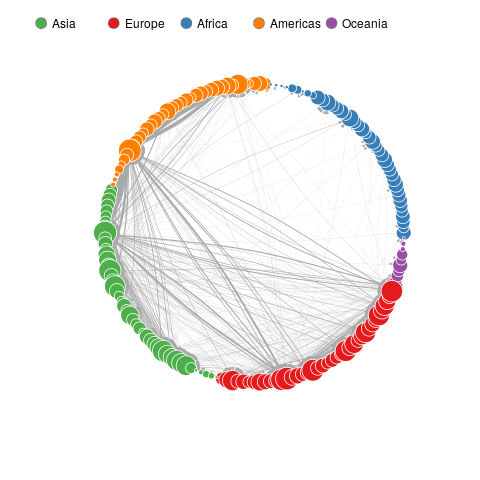
\includegraphics[width=0.45\linewidth]{grafo_2016_1_pcnt_wgt_Circ}}
	\subfigure[5\%]{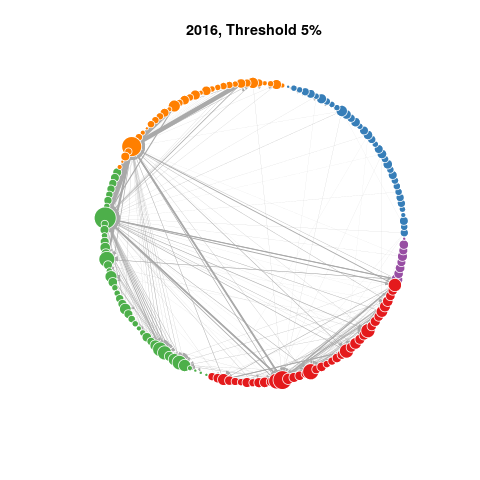
\includegraphics[width=0.45\linewidth]{grafo_2016_5_pcnt_wgt_Circ}}
	\subfigure[10\%]{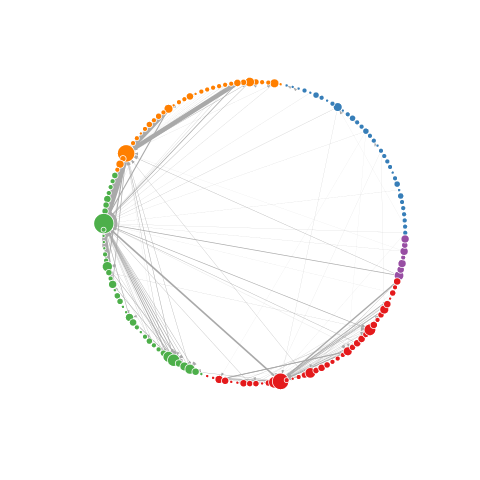
\includegraphics[width=0.45\linewidth]{grafo_2016_10_pcnt_wgt_Circ}}
	\subfigure[15\%]{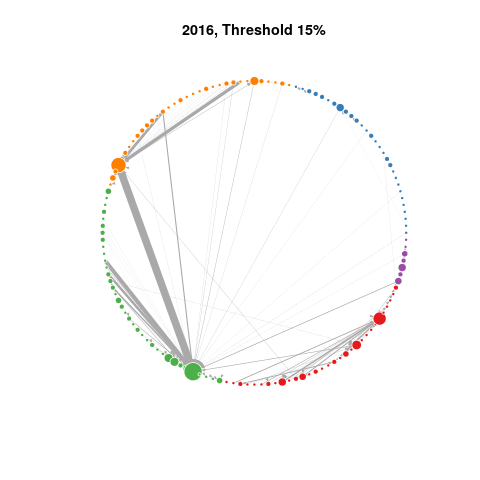
\includegraphics[width=0.45\linewidth]{grafo_2016_15_pcnt_wgt_Circ}}
	\subfigure[20\%]{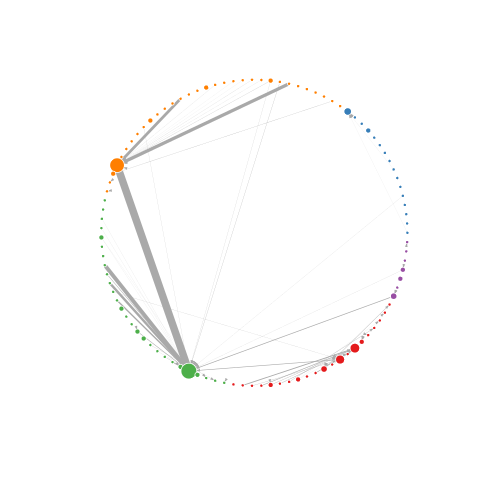
\includegraphics[width=0.45\linewidth]{grafo_2016_20_pcnt_wgt_Circ}}
	\subfigure[25\%]{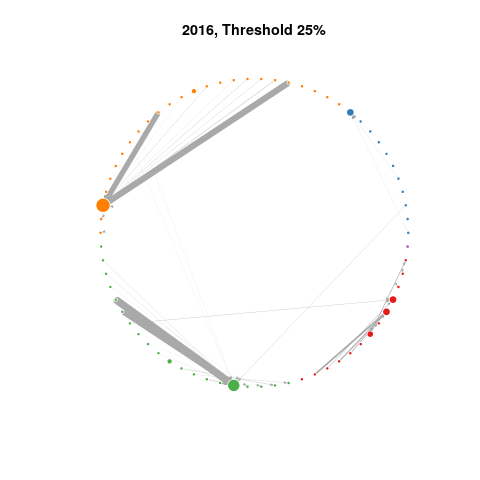
\includegraphics[width=0.45\linewidth]{grafo_2016_25_pcnt_wgt_Circ}}
	\caption{Grafos. 2016, según punto de corte. Ponderado por Valor comercial. Importaciones}
	\label{fig:grafo_2016_circular}
\end{figure}


\begin{figure}
	\centering
	\subfigure[1\%]{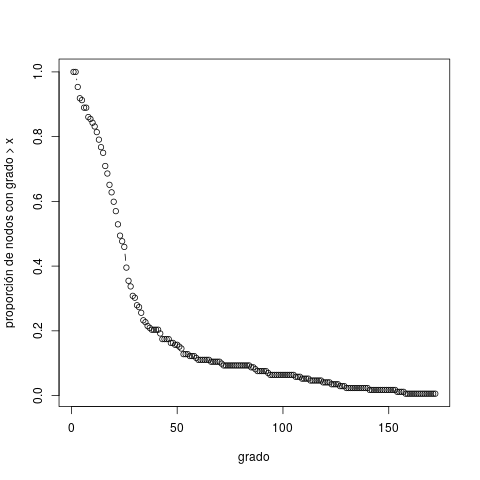
\includegraphics[width=0.45\linewidth]{dist_ac_2016_1_pcnt}}
	\subfigure[5\%]{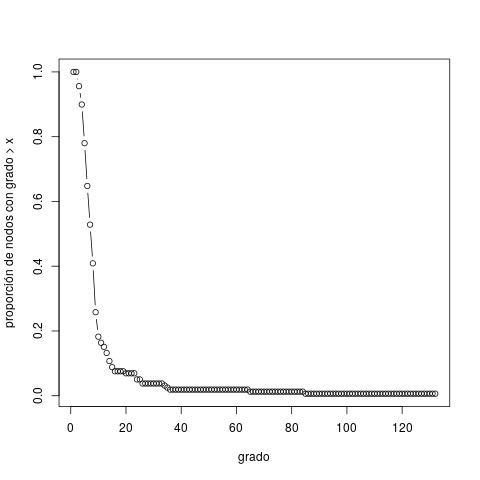
\includegraphics[width=0.45\linewidth]{dist_ac_2016_5_pcnt}}
	\subfigure[10\%]{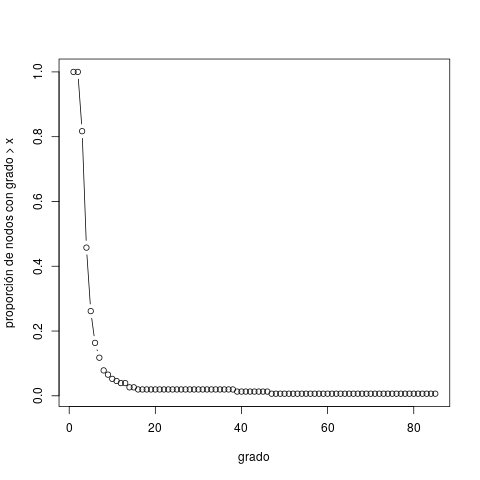
\includegraphics[width=0.45\linewidth]{dist_ac_2016_10_pcnt}}
	\subfigure[15\%]{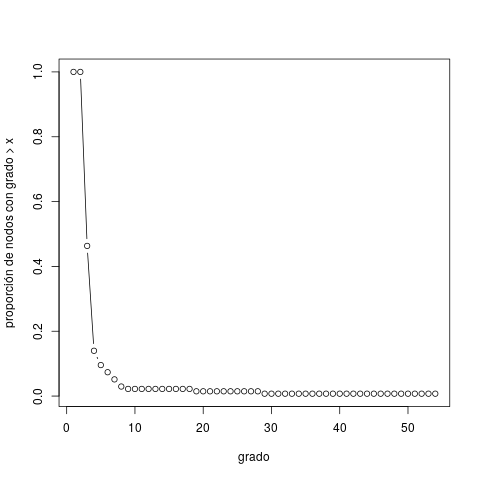
\includegraphics[width=0.45\linewidth]{dist_ac_2016_15_pcnt}}
	\subfigure[20\%]{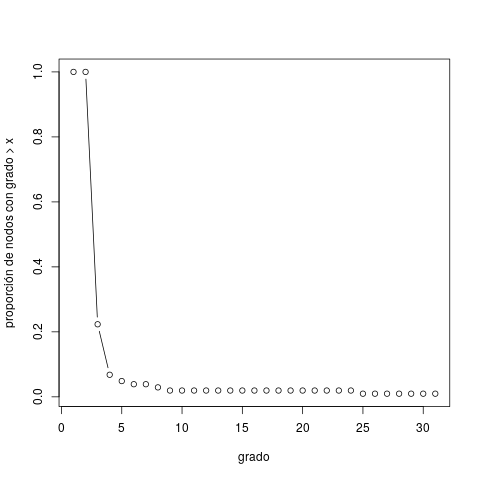
\includegraphics[width=0.45\linewidth]{dist_ac_2016_20_pcnt}}
	\subfigure[25\%]{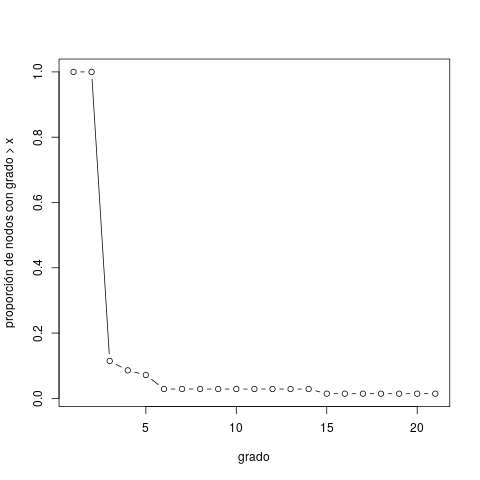
\includegraphics[width=0.45\linewidth]{dist_ac_2016_25_pcnt}}
	\caption{Distribución acumulada del grado. 2016, según punto de corte. Importaciones}
	\label{fig:dist_ac_grado}
\end{figure}

\begin{figure}
	\centering
	\subfigure[5\%]{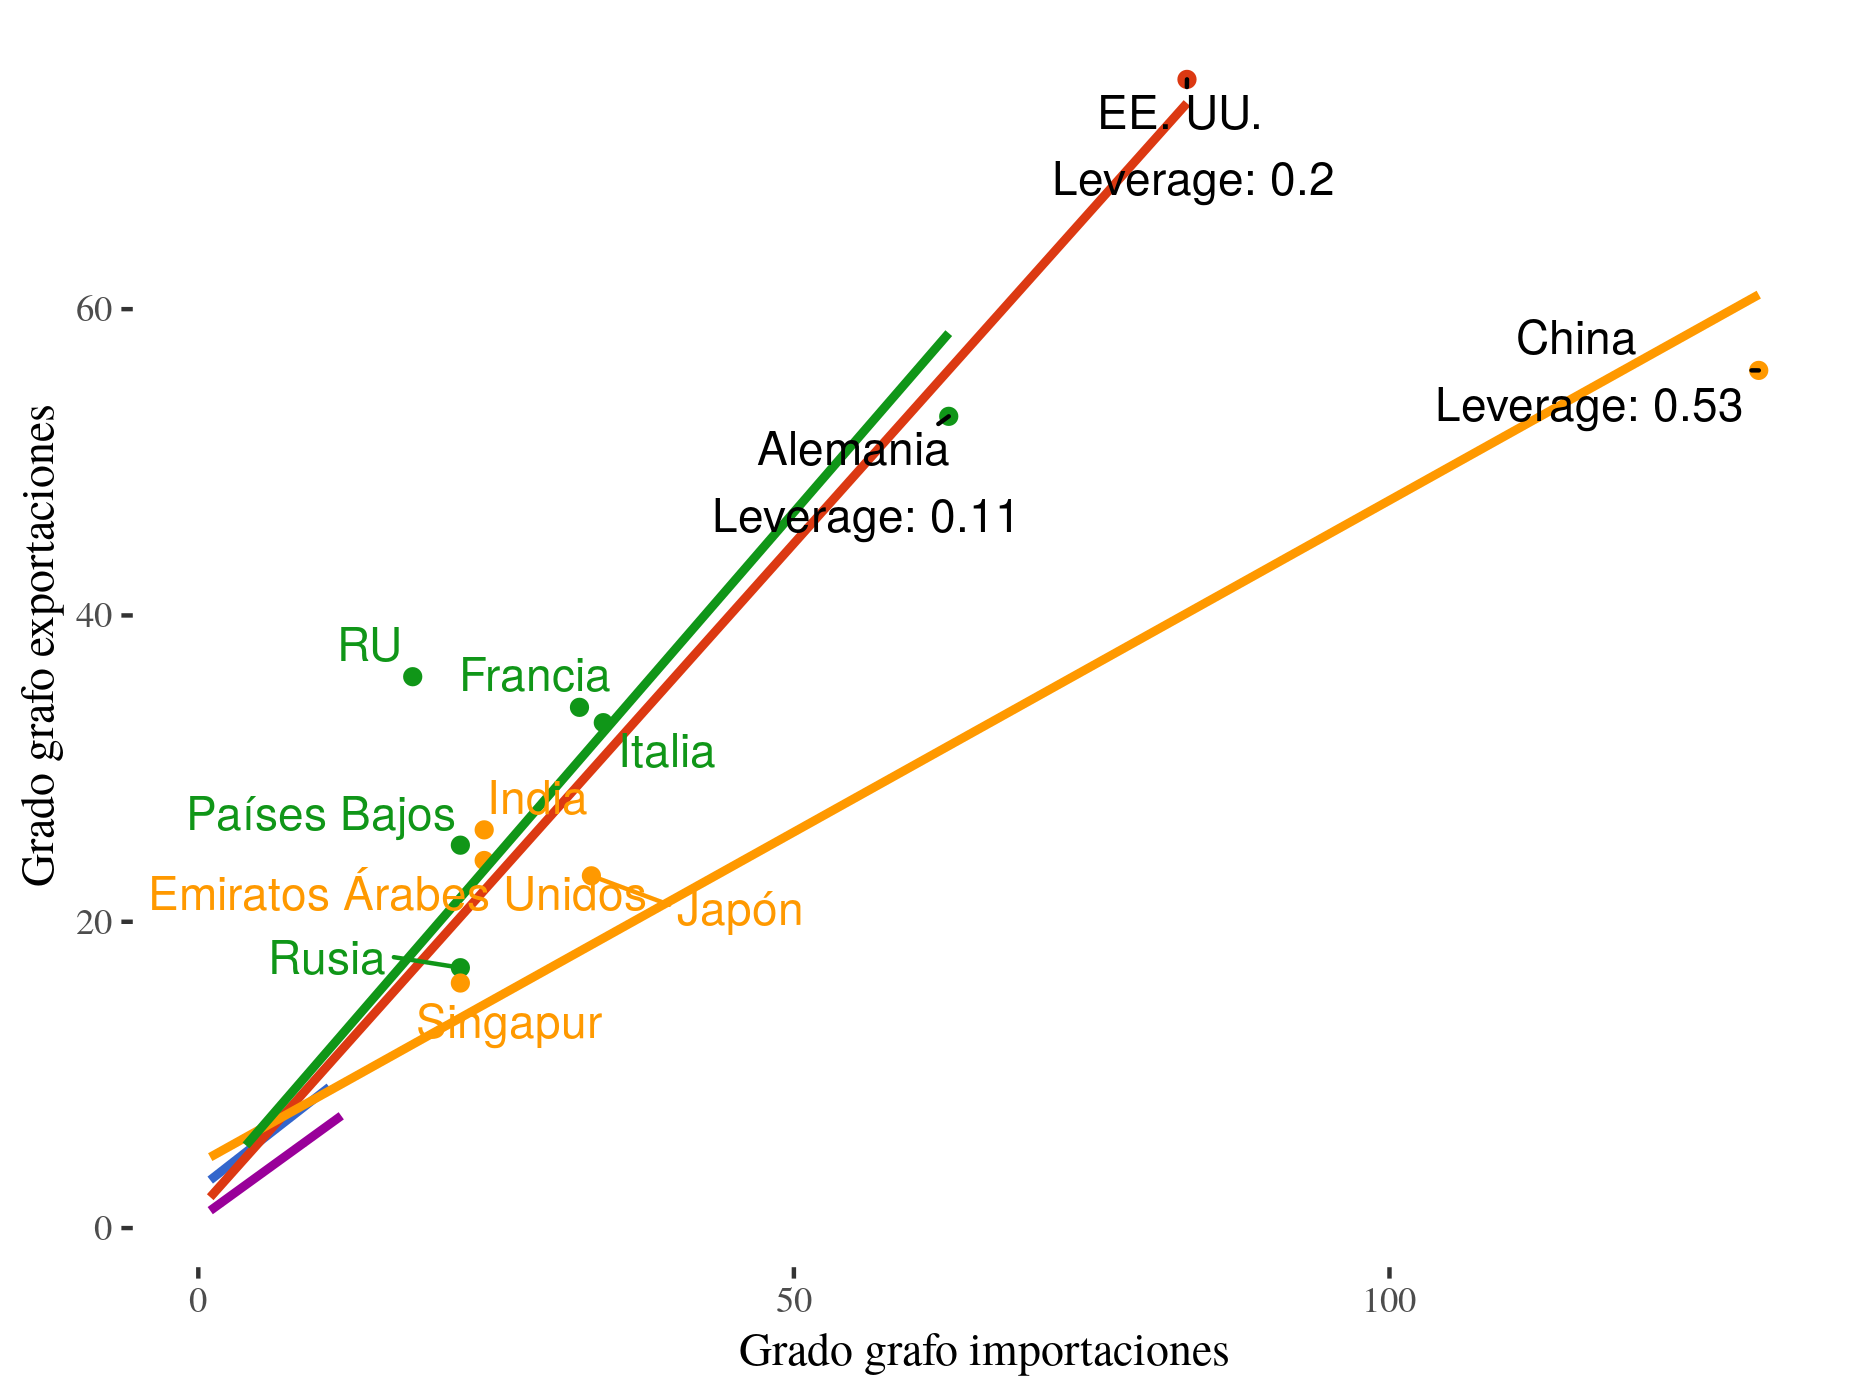
\includegraphics[width=0.48\linewidth]{corr_grados_2016_5_pcnt}}
	\subfigure[15\%]{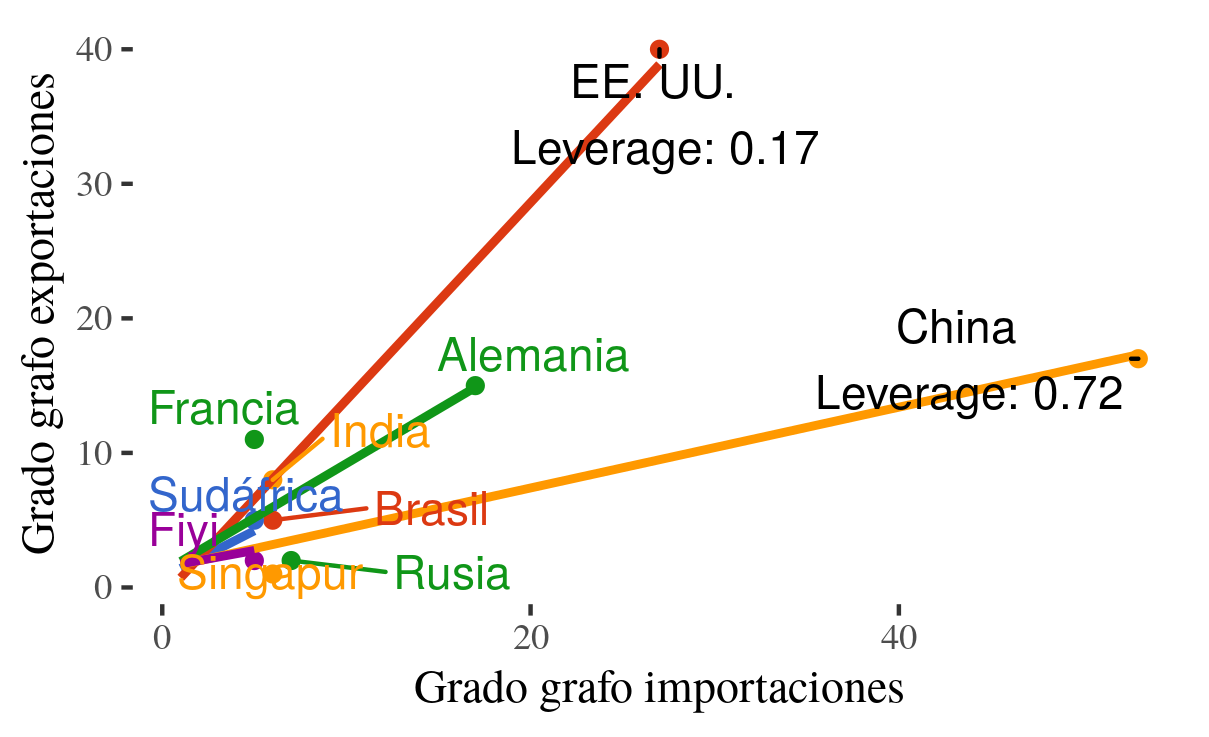
\includegraphics[width=0.48\linewidth]{corr_grados_2016_15_pcnt}}
	\subfigure[25\%]{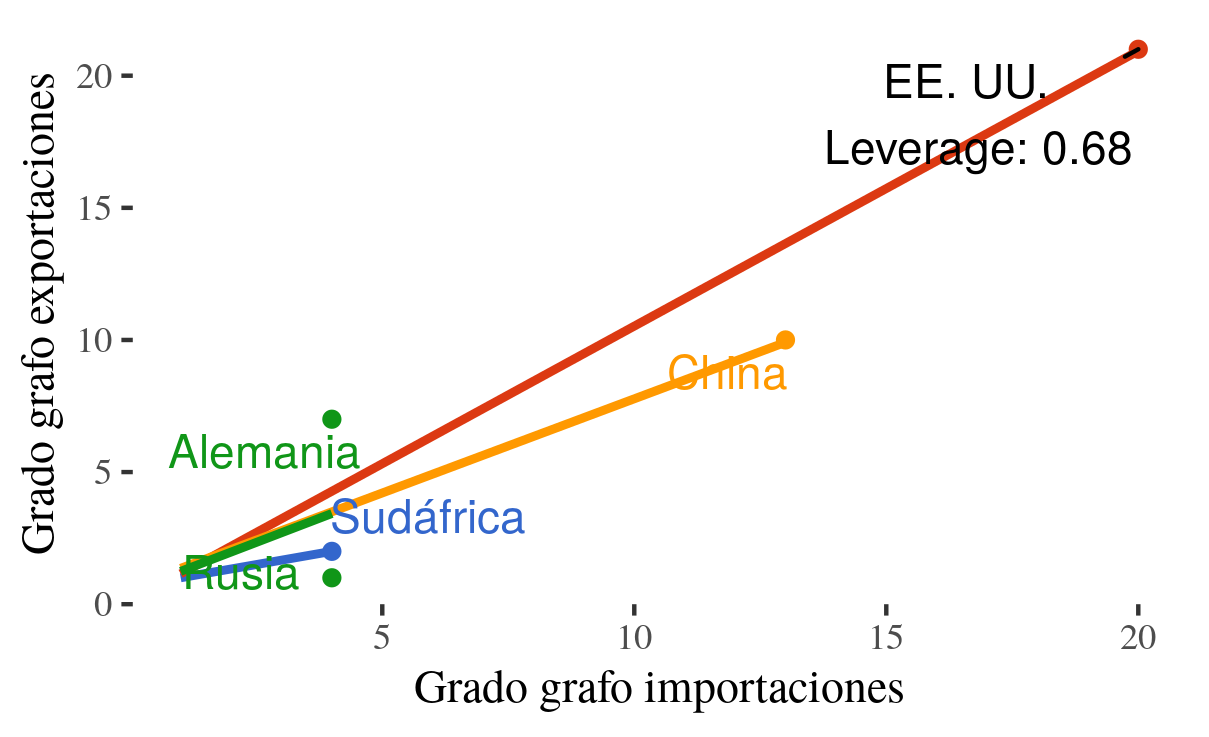
\includegraphics[width=0.48\linewidth]{corr_grados_2016_25_pcnt}}
	\caption{Grado total. Grafo exportaciones respecto grafo importaciones. Año 2016}
	\label{fig:corr_comp}
\end{figure}


\begin{figure}
	\centering
	\subfigure[Número de aristas]{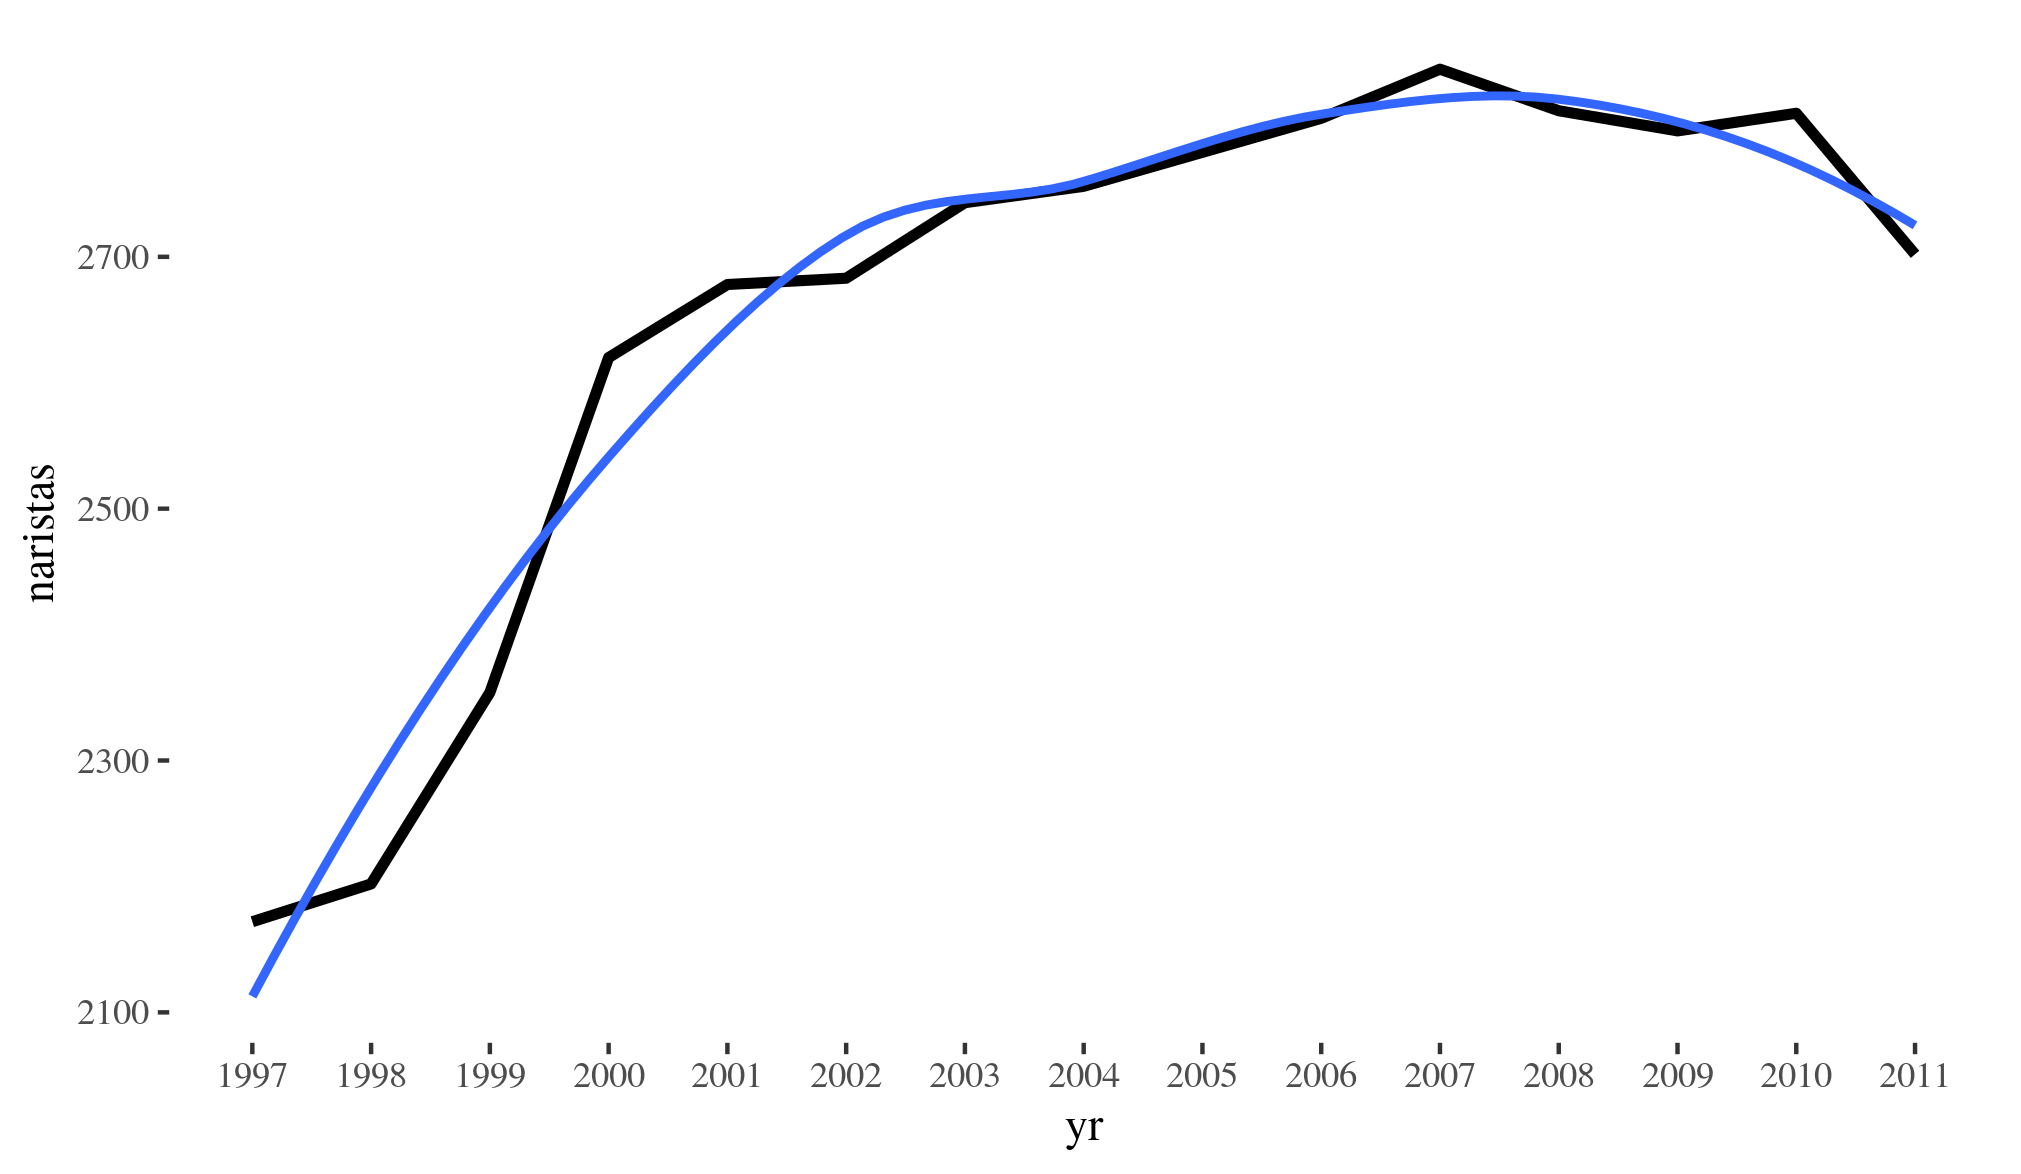
\includegraphics[width=.45\linewidth]{naristas_x_yr}}
	\subfigure[Grado promedio]{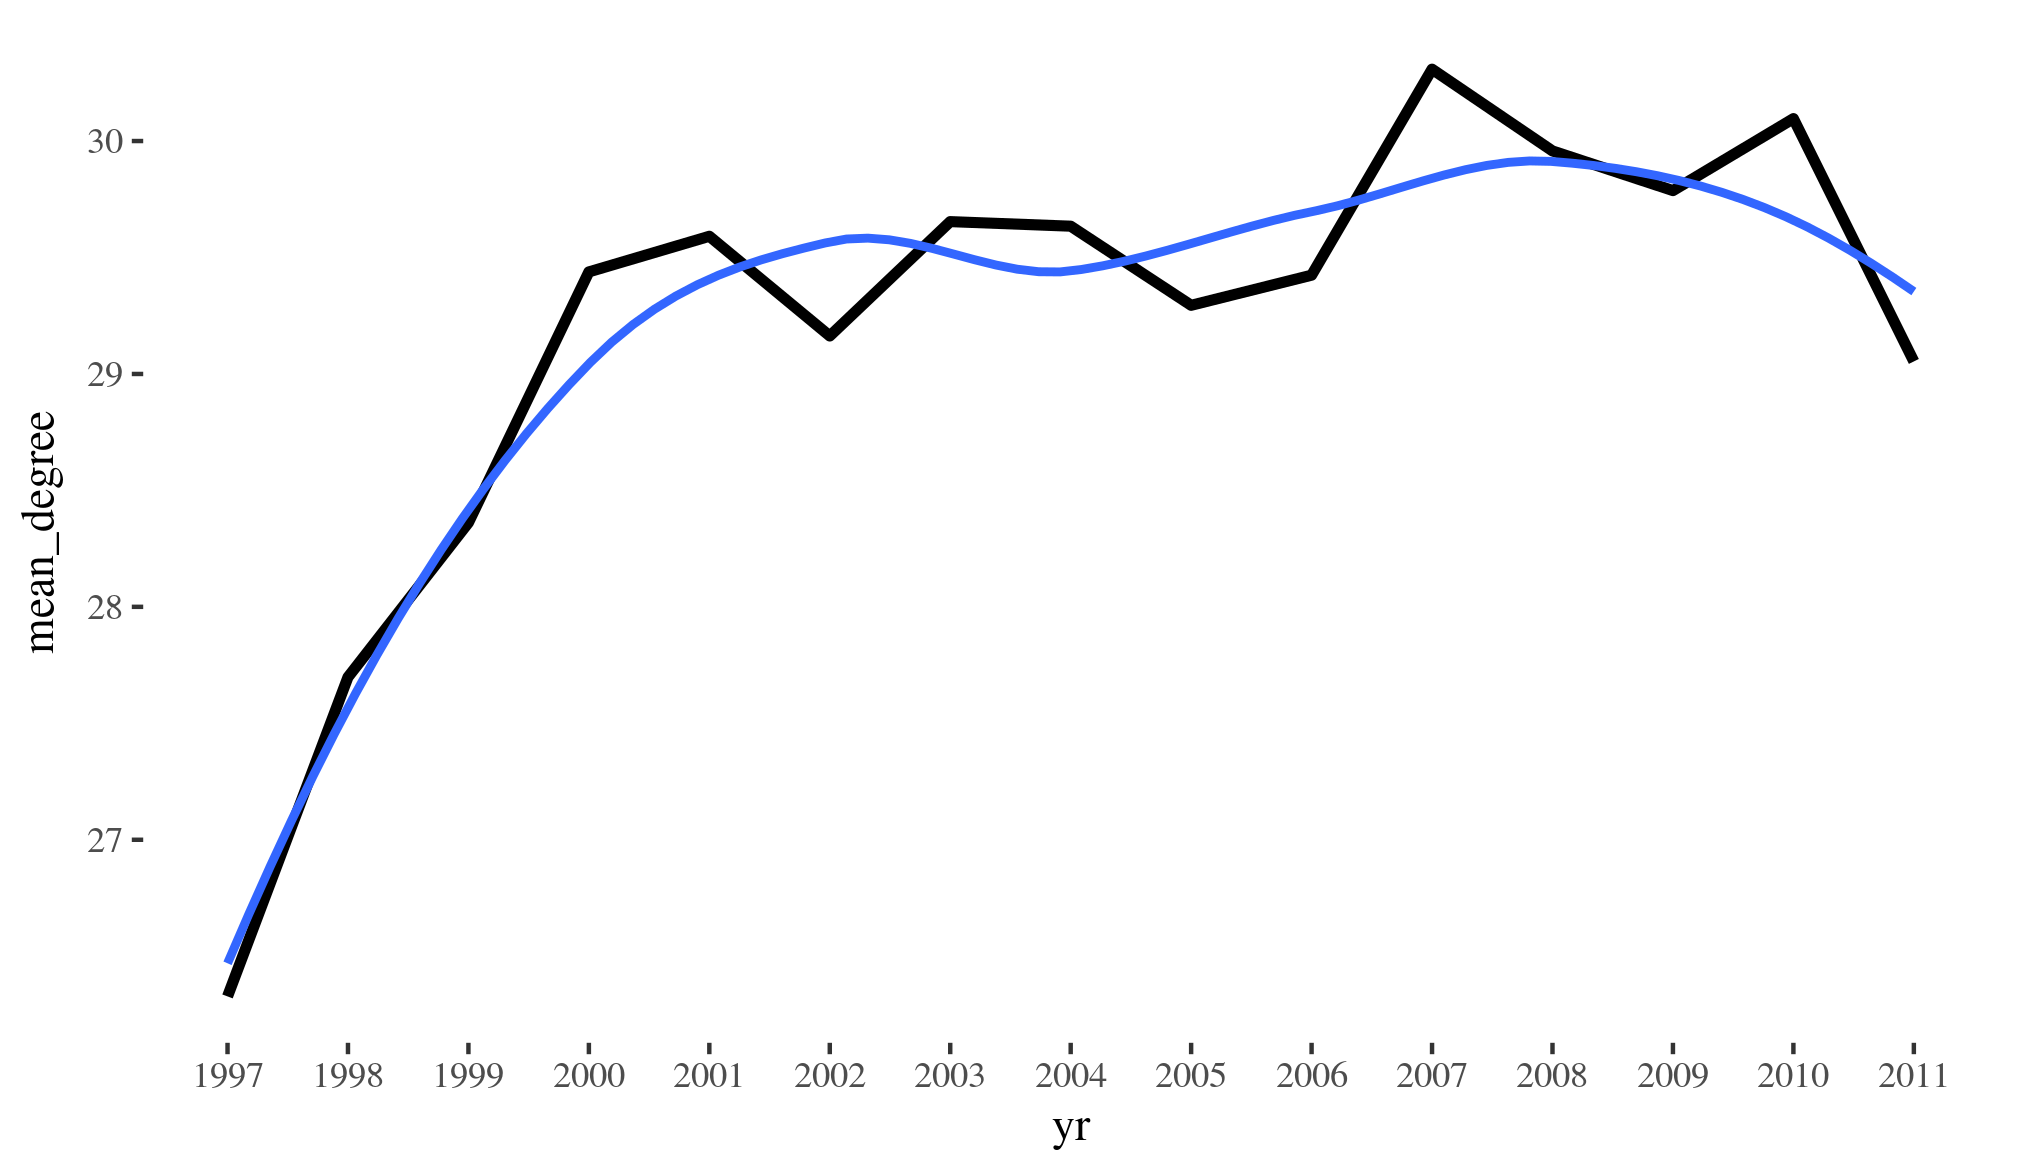
\includegraphics[width=.45\linewidth]{mean_degree_x_yr}}
	\subfigure[Cercanía promedio]{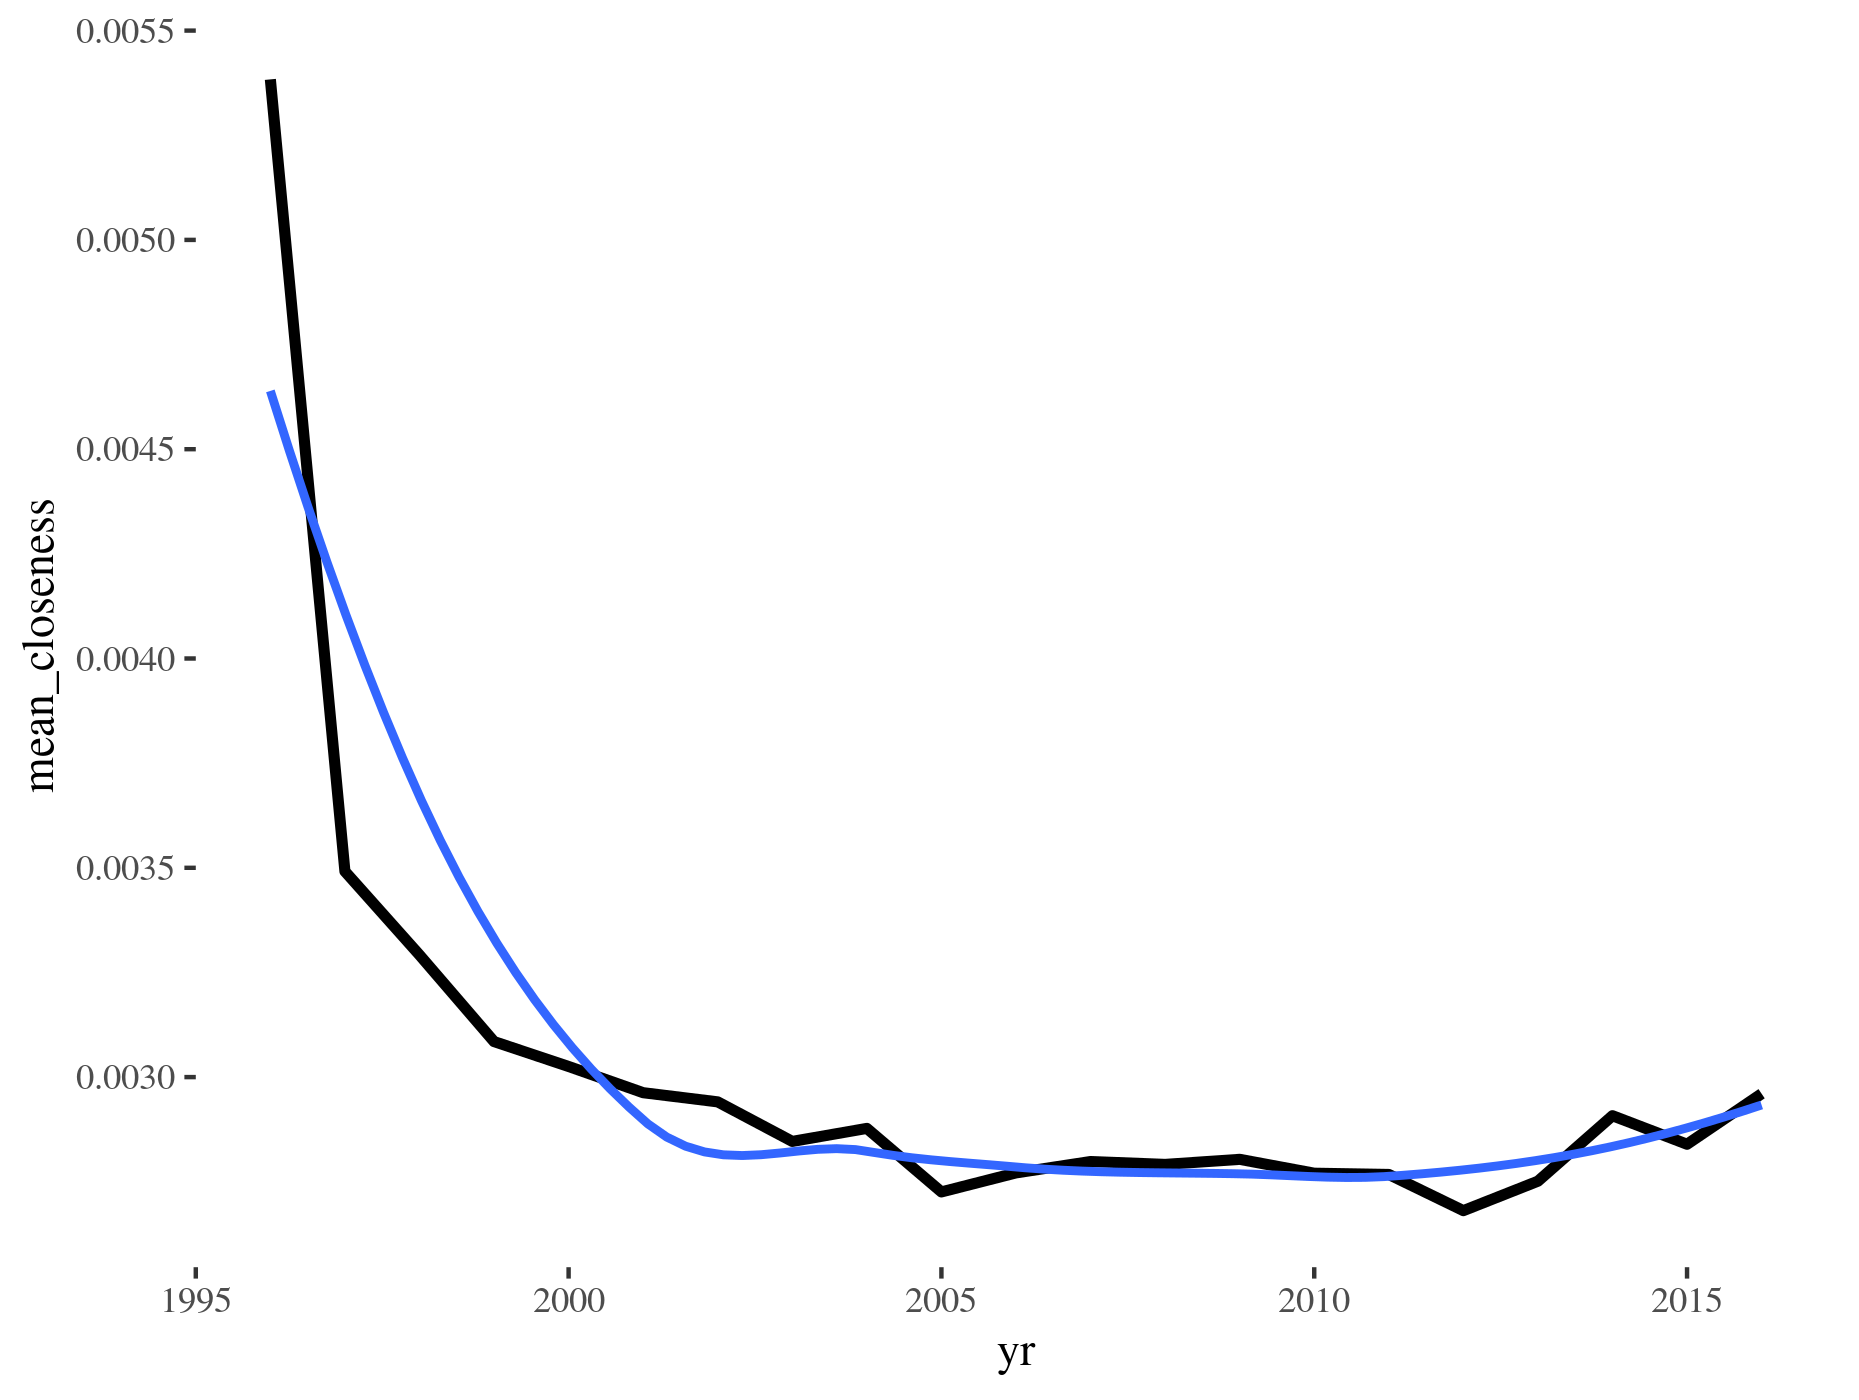
\includegraphics[width=.45\linewidth]{mean_closeness_x_yr}}
	\subfigure[Máxima intermediación]{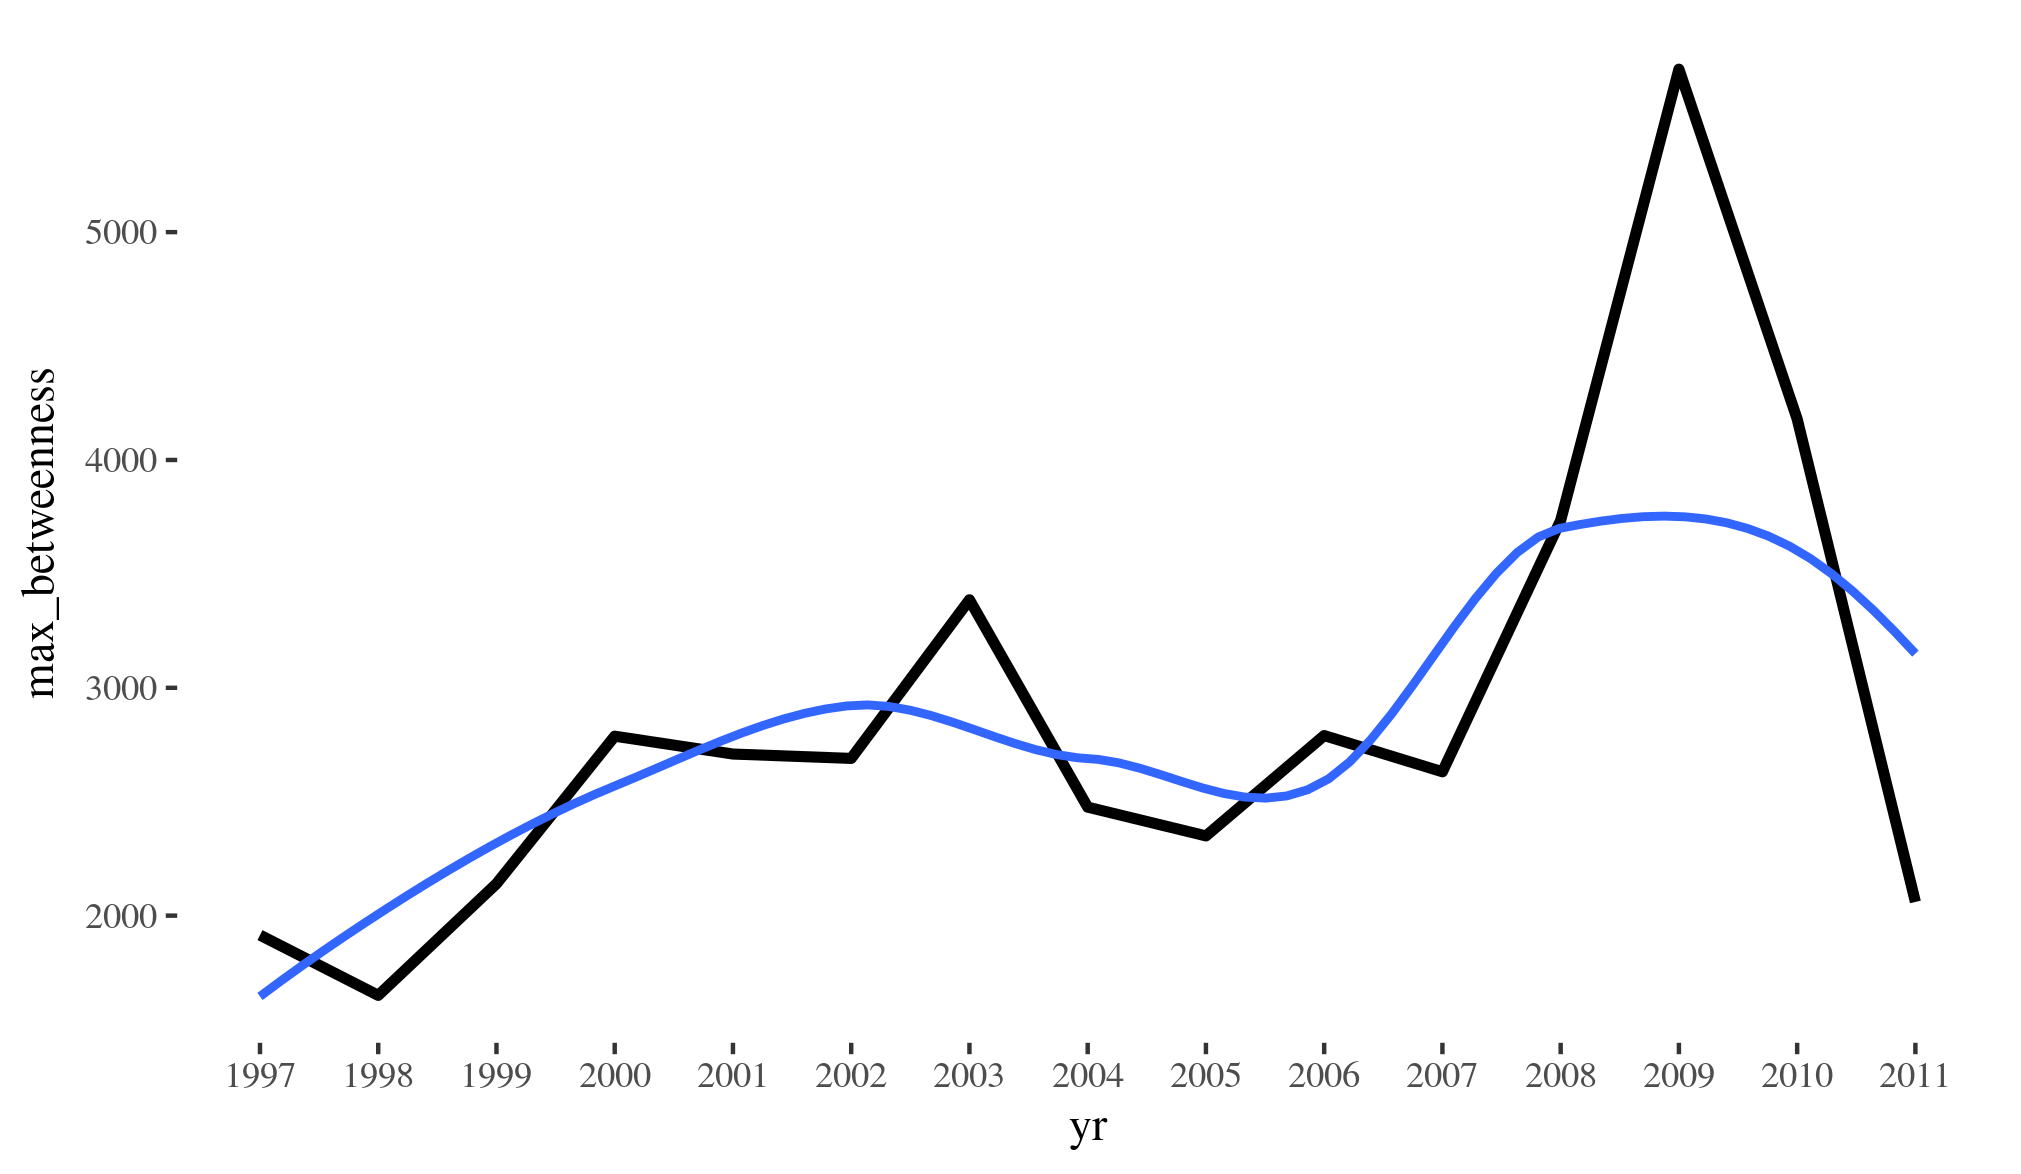
\includegraphics[width=.45\linewidth]{max_betweenness_x_yr}}
	\subfigure[Intermediación promedio]{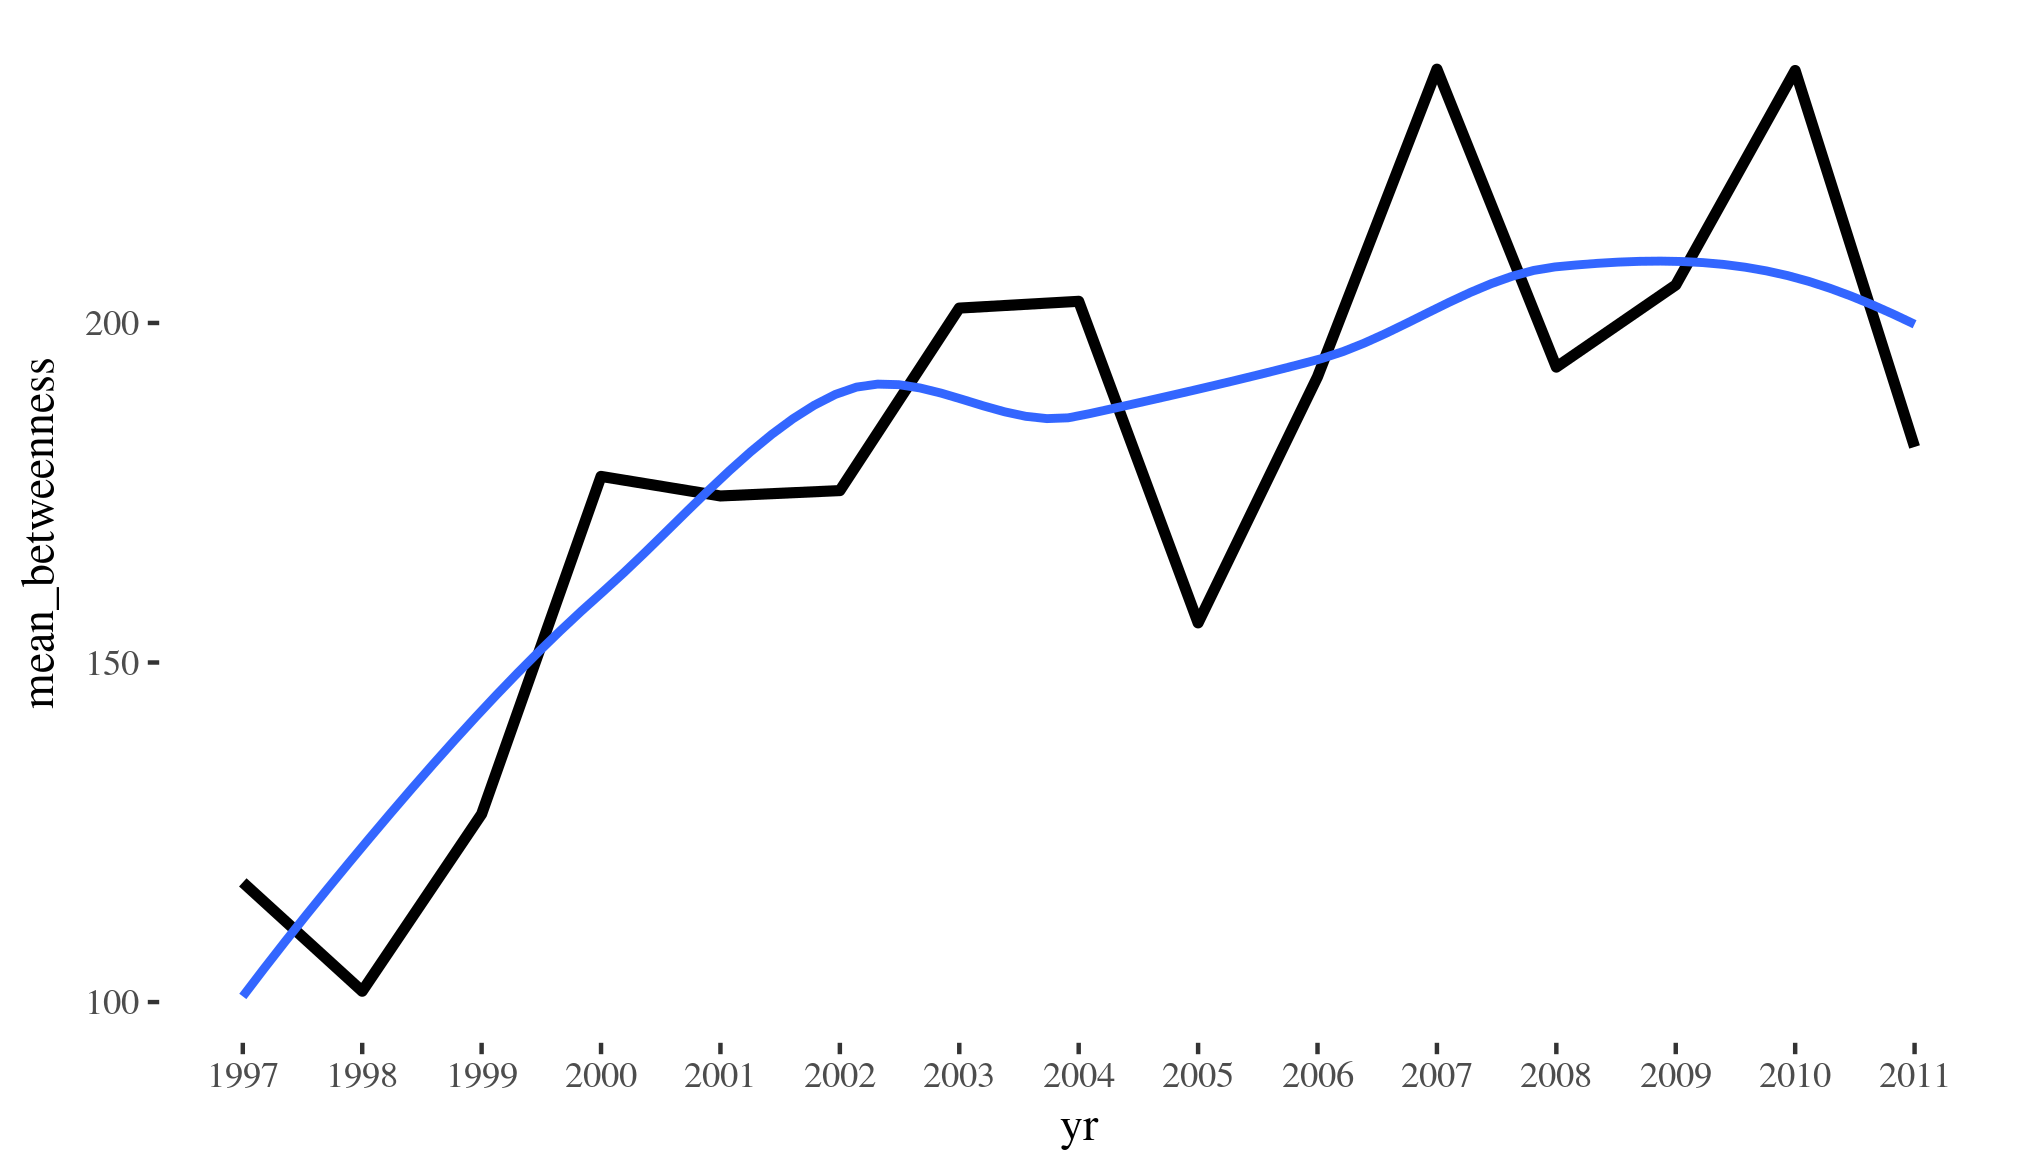
\includegraphics[width=.45\linewidth]{mean_betweenness_x_yr}}
	\subfigure[Autovalor promedio]{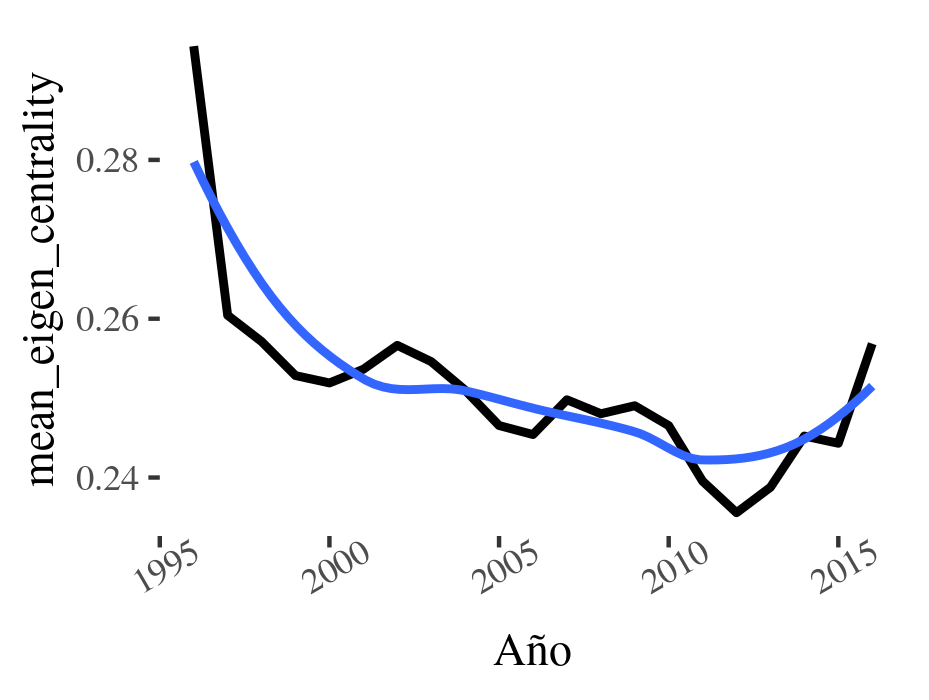
\includegraphics[width=.45\linewidth]{mean_eigen_centrality_x_yr}}
	\subfigure[Autovalor promedio. Ponderado por valor comercial]{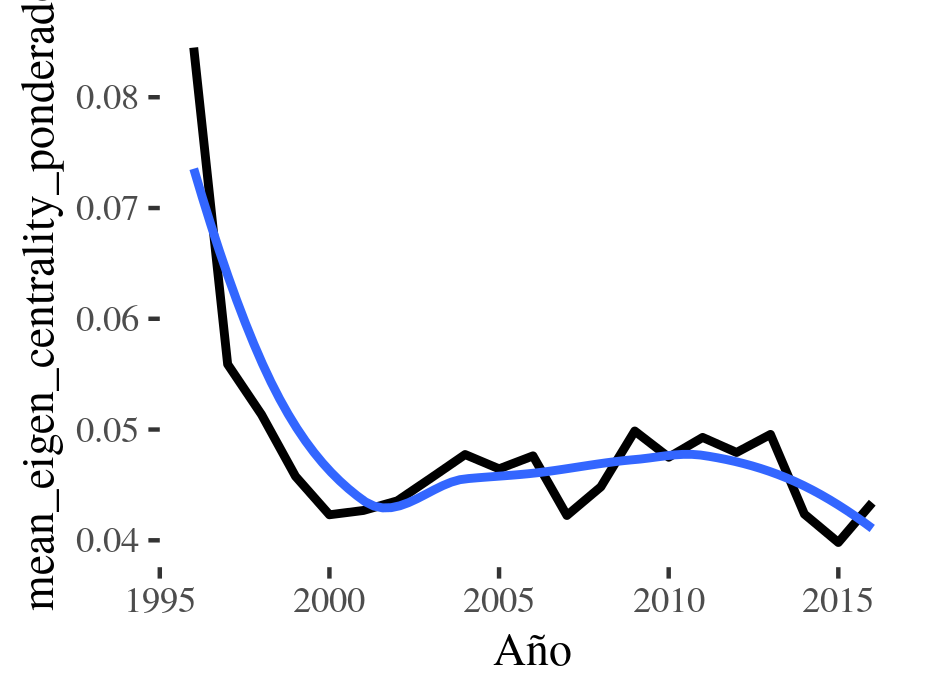
\includegraphics[width=.45\linewidth]{mean_eigen_centrality_ponderado_x_yr}}
	\caption{Importaciones. Umbral 1\%. 1996-2016}
	\label{fig:caracteristicas_yr_comp}
\end{figure}


\begin{figure}[h!]
	\centering
	\subfigure[Número de aristas]{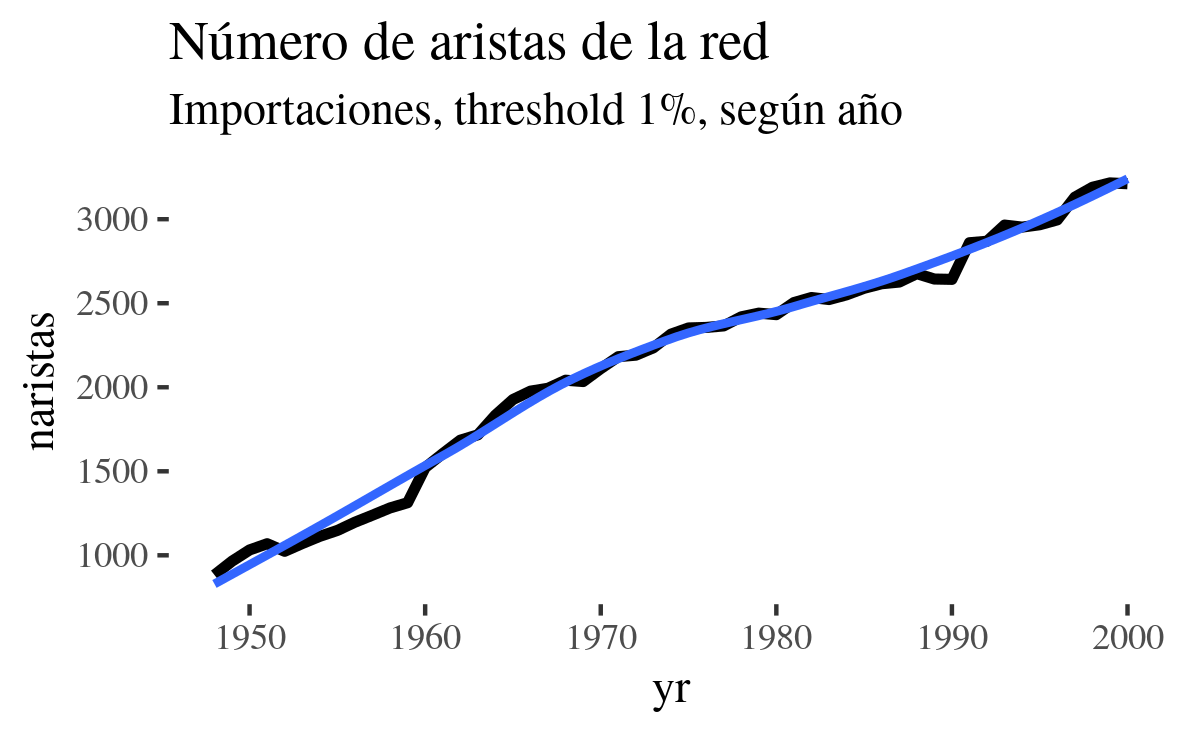
\includegraphics[width=.45\linewidth]{1950_2000_naristas_x_yr}}
	\subfigure[Diámetro]{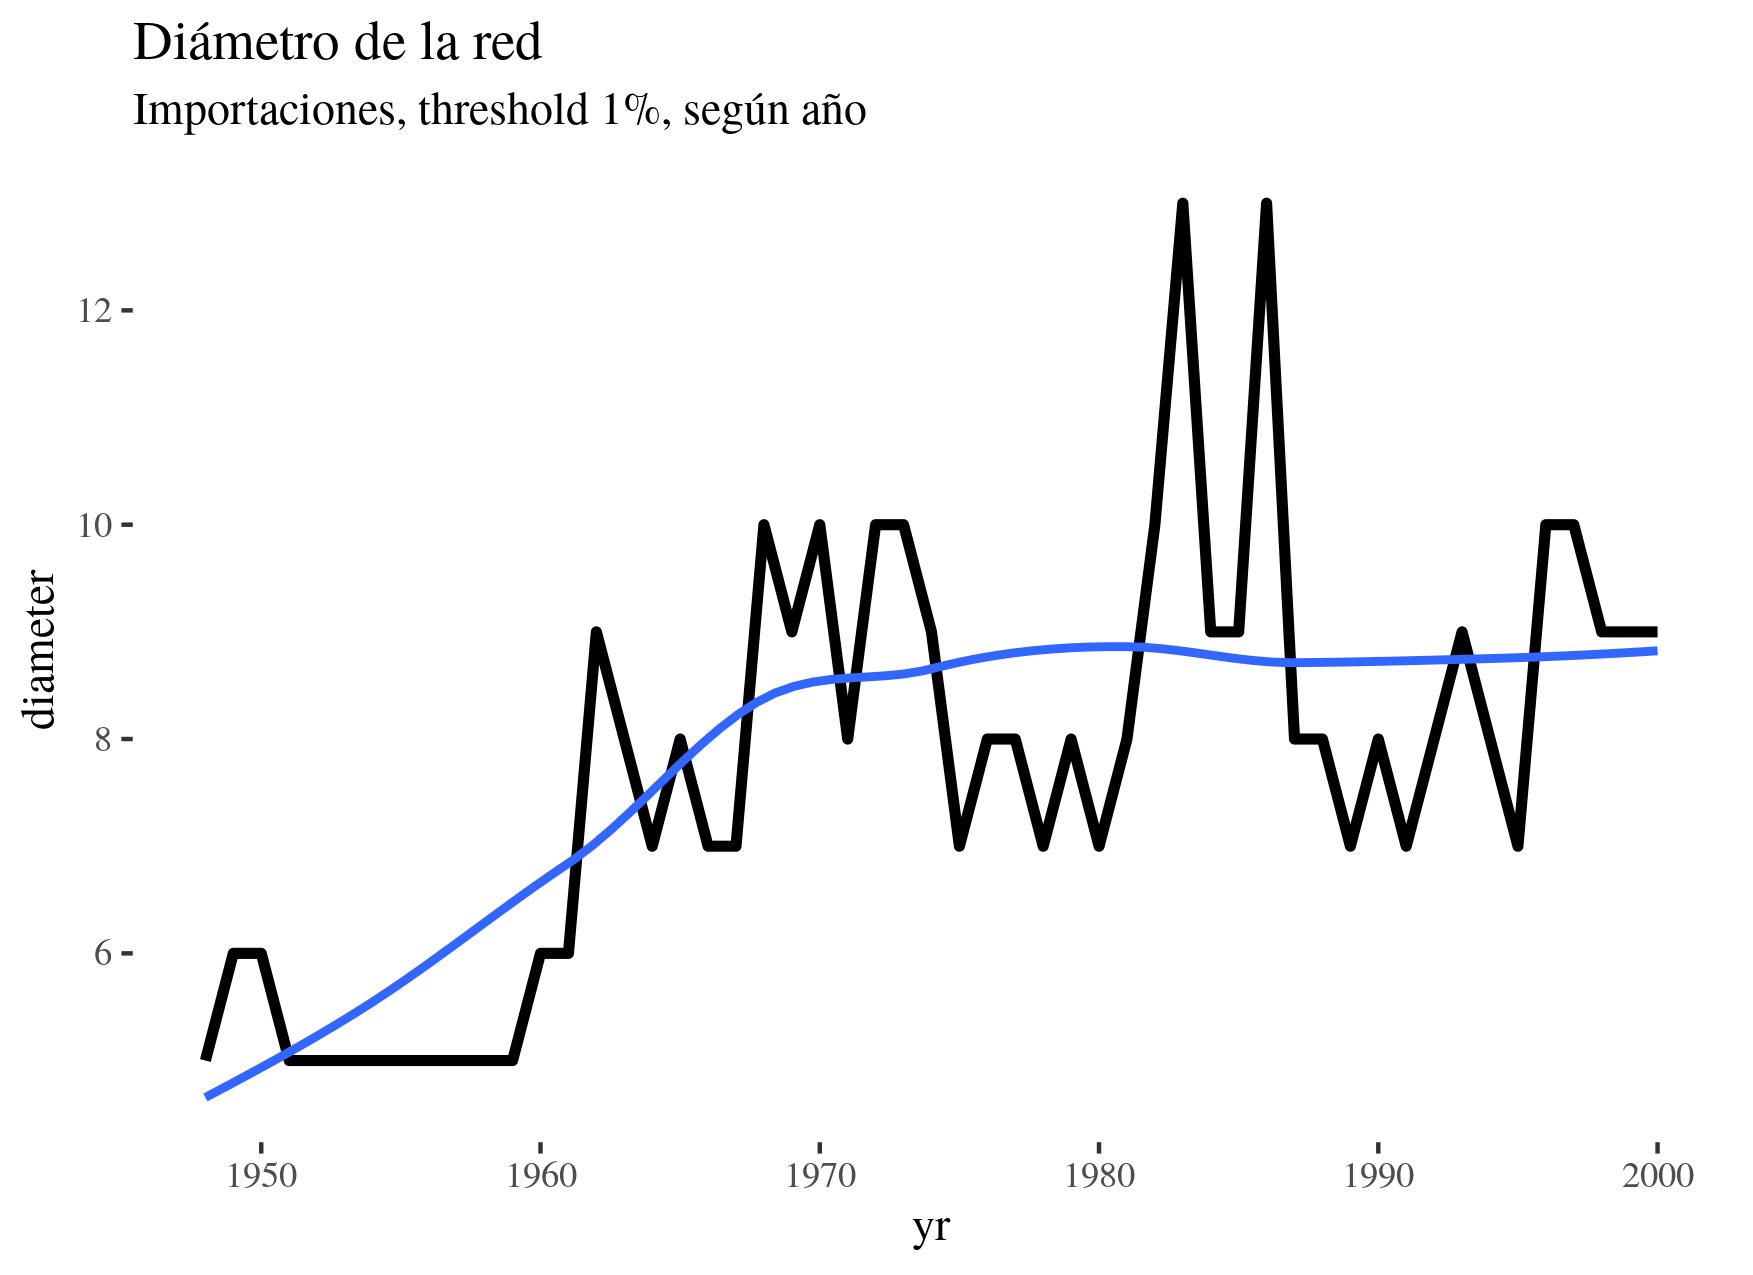
\includegraphics[width=.45\linewidth]{1950_2000_diametro_x_ano}}	\subfigure[Correlación]{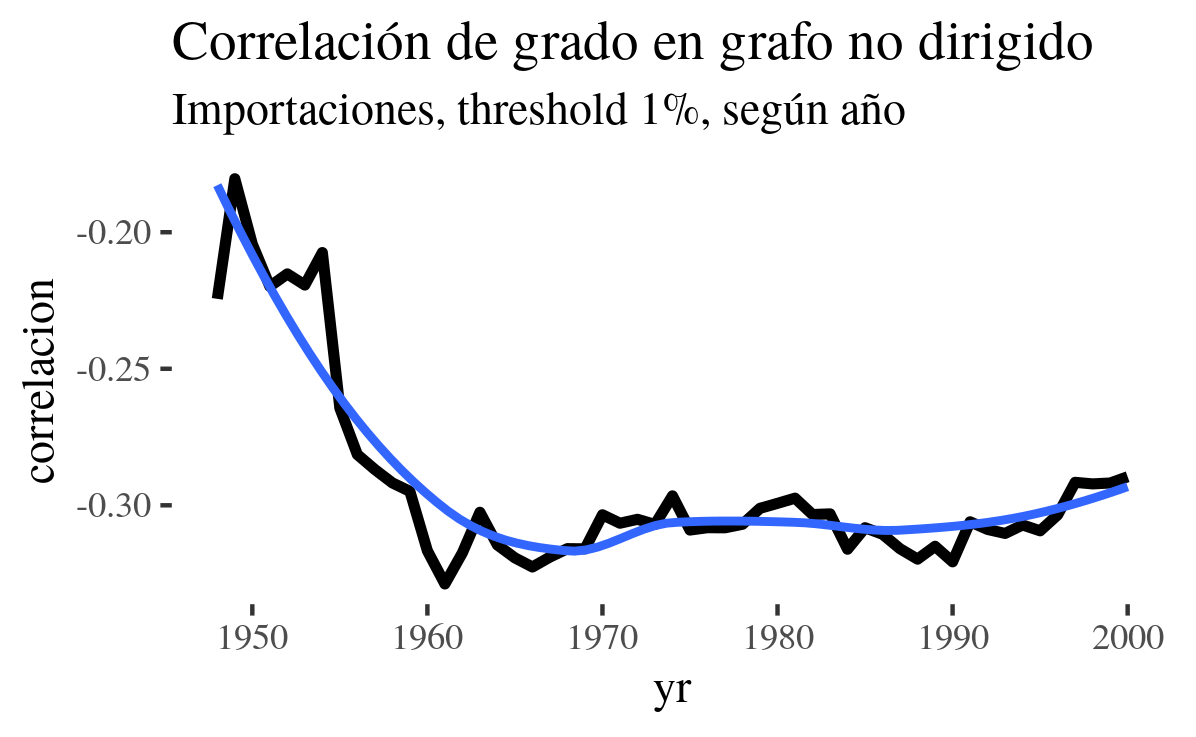
\includegraphics[width=.45\linewidth]{1950_2000_correlacion_x_yr}}	\subfigure[Grado medio]{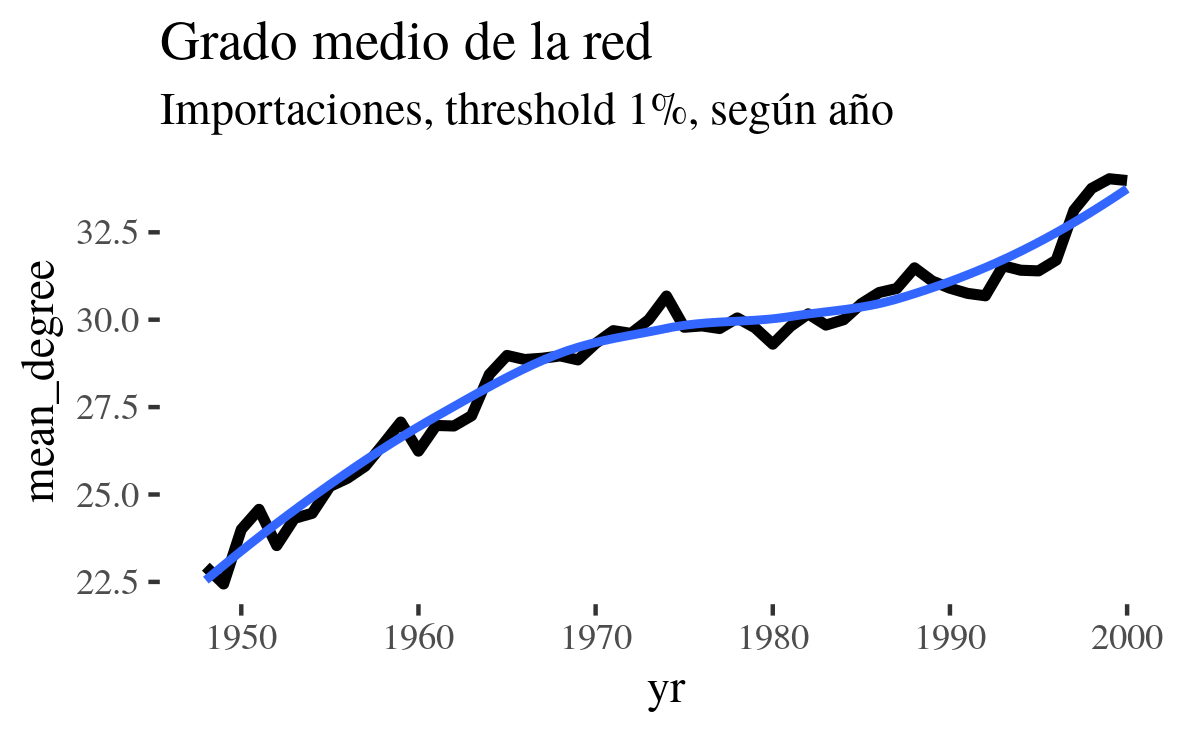
\includegraphics[width=.45\linewidth]{1950_2000_mean_degree_x_yr}}	\subfigure[cercanía promedio]{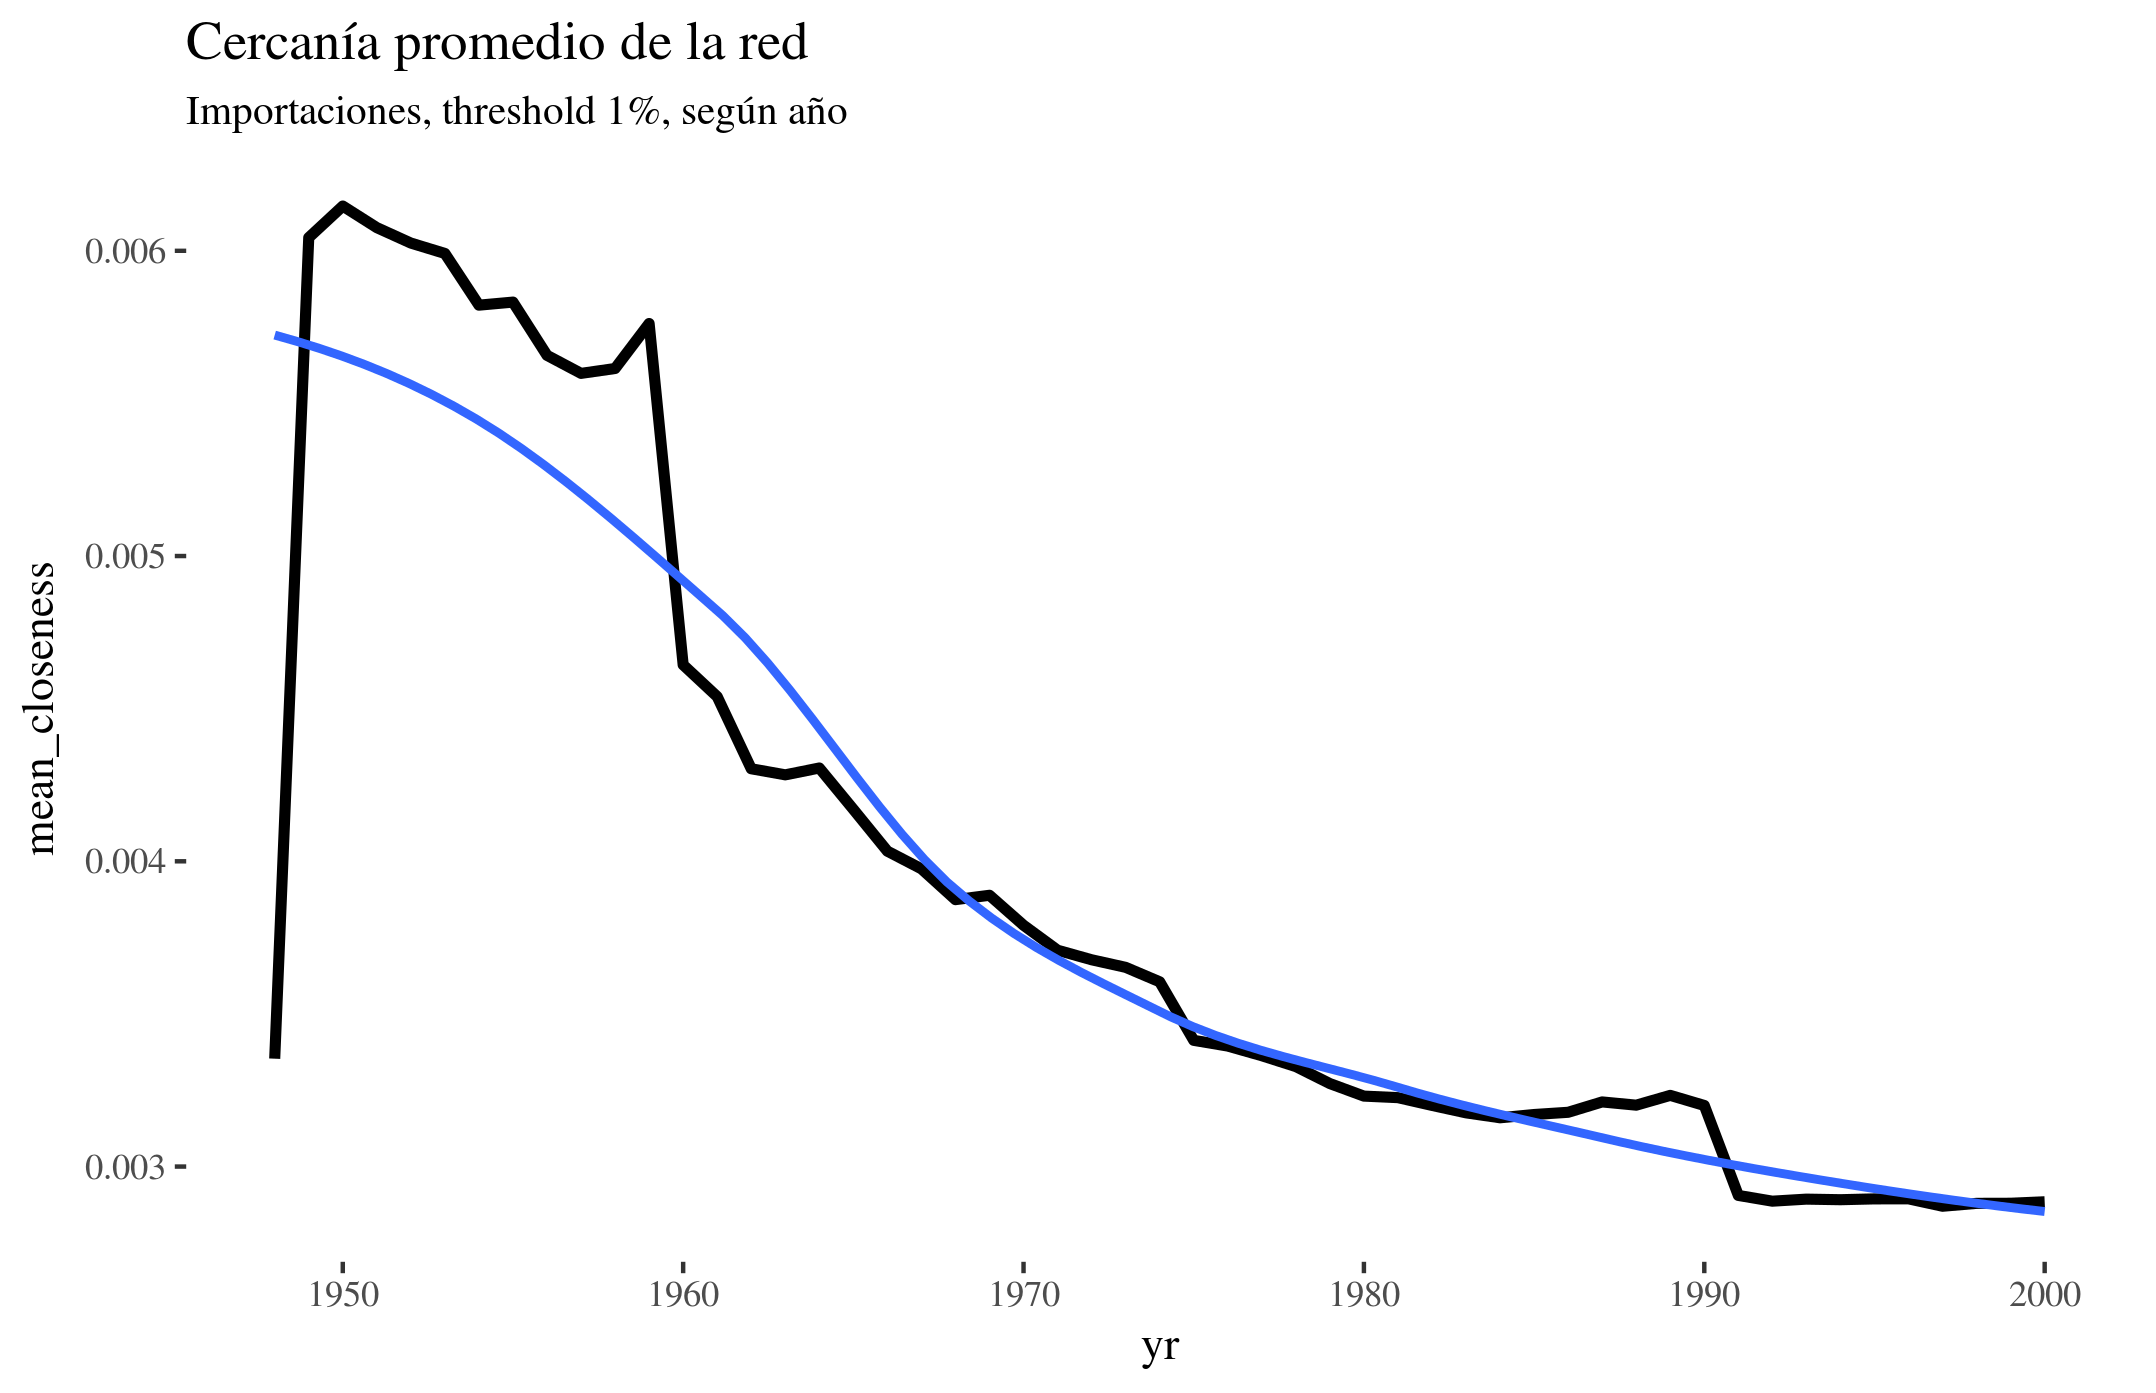
\includegraphics[width=.45\linewidth]{1950_2000_mean_closeness_x_yr}}		\caption{Evolución de la estructura de la red. Importaciones. Umbral 1\%.1948-2000}
	\label{fig:metricas_LP_comp}
\end{figure}

\begin{figure}[h!]
	\centering
	\subfigure[Intermediación máxima]{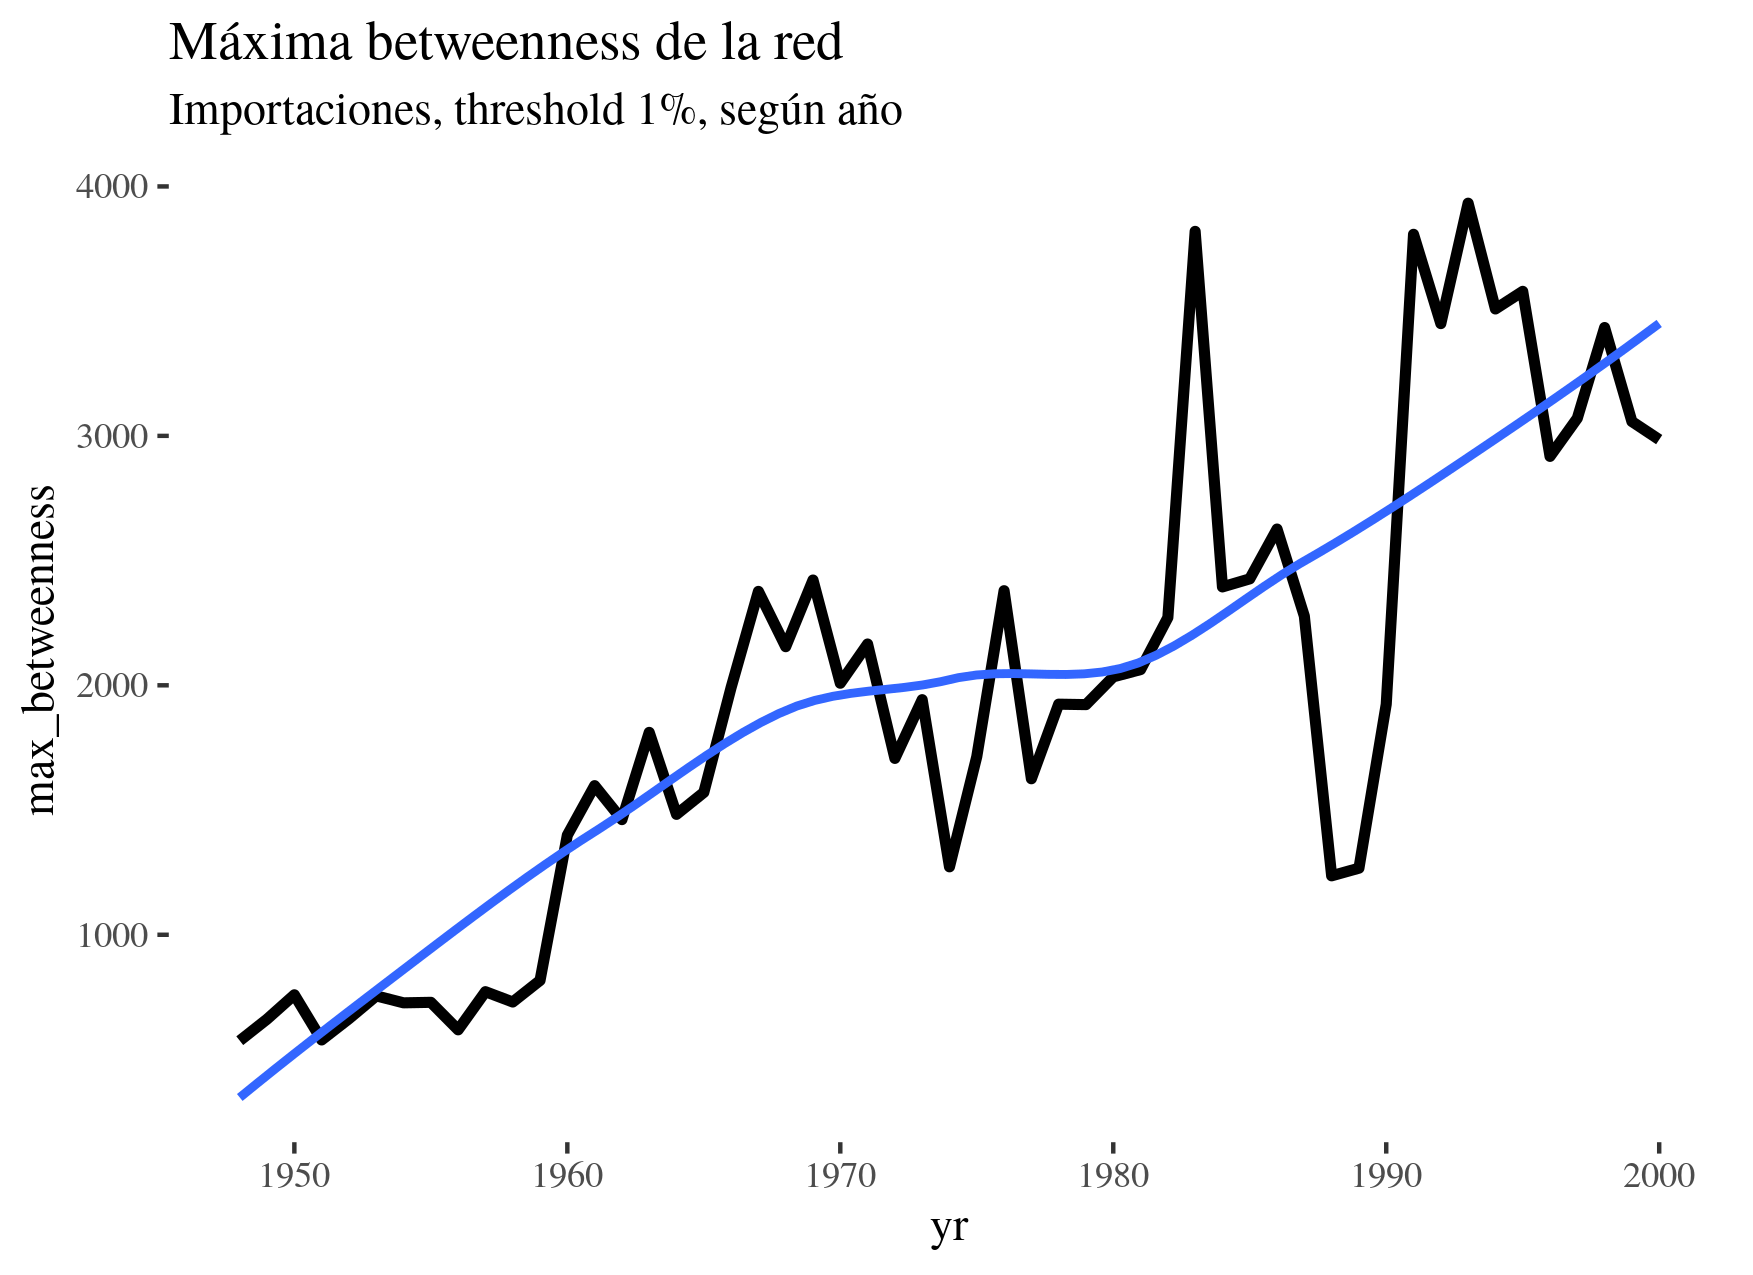
\includegraphics[width=.45\linewidth]{1950_2000_max_betweenness_x_yr}}	
	\subfigure[Intermediación media]{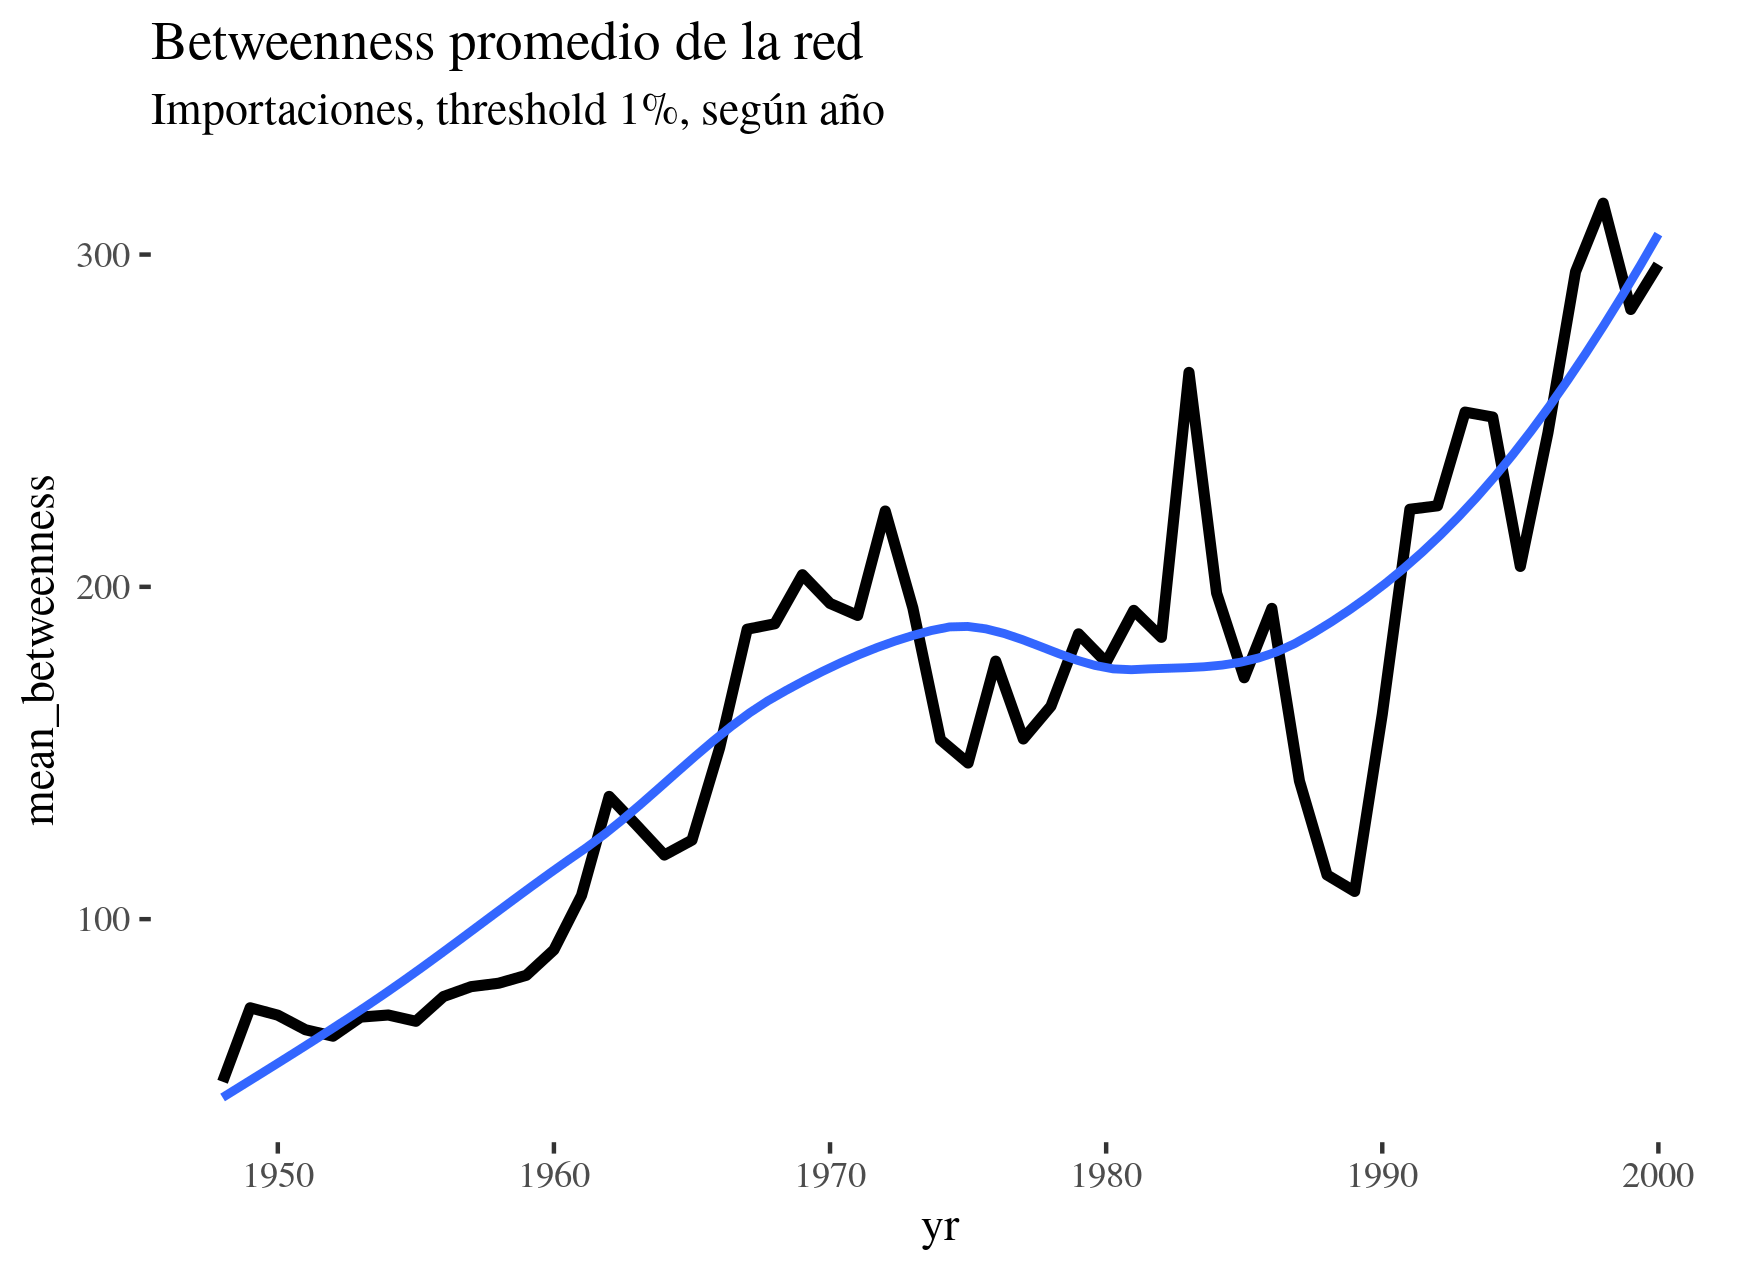
\includegraphics[width=.45\linewidth]{1950_2000_mean_betweenness_x_yr}}
	\subfigure[Autovalor promedio]{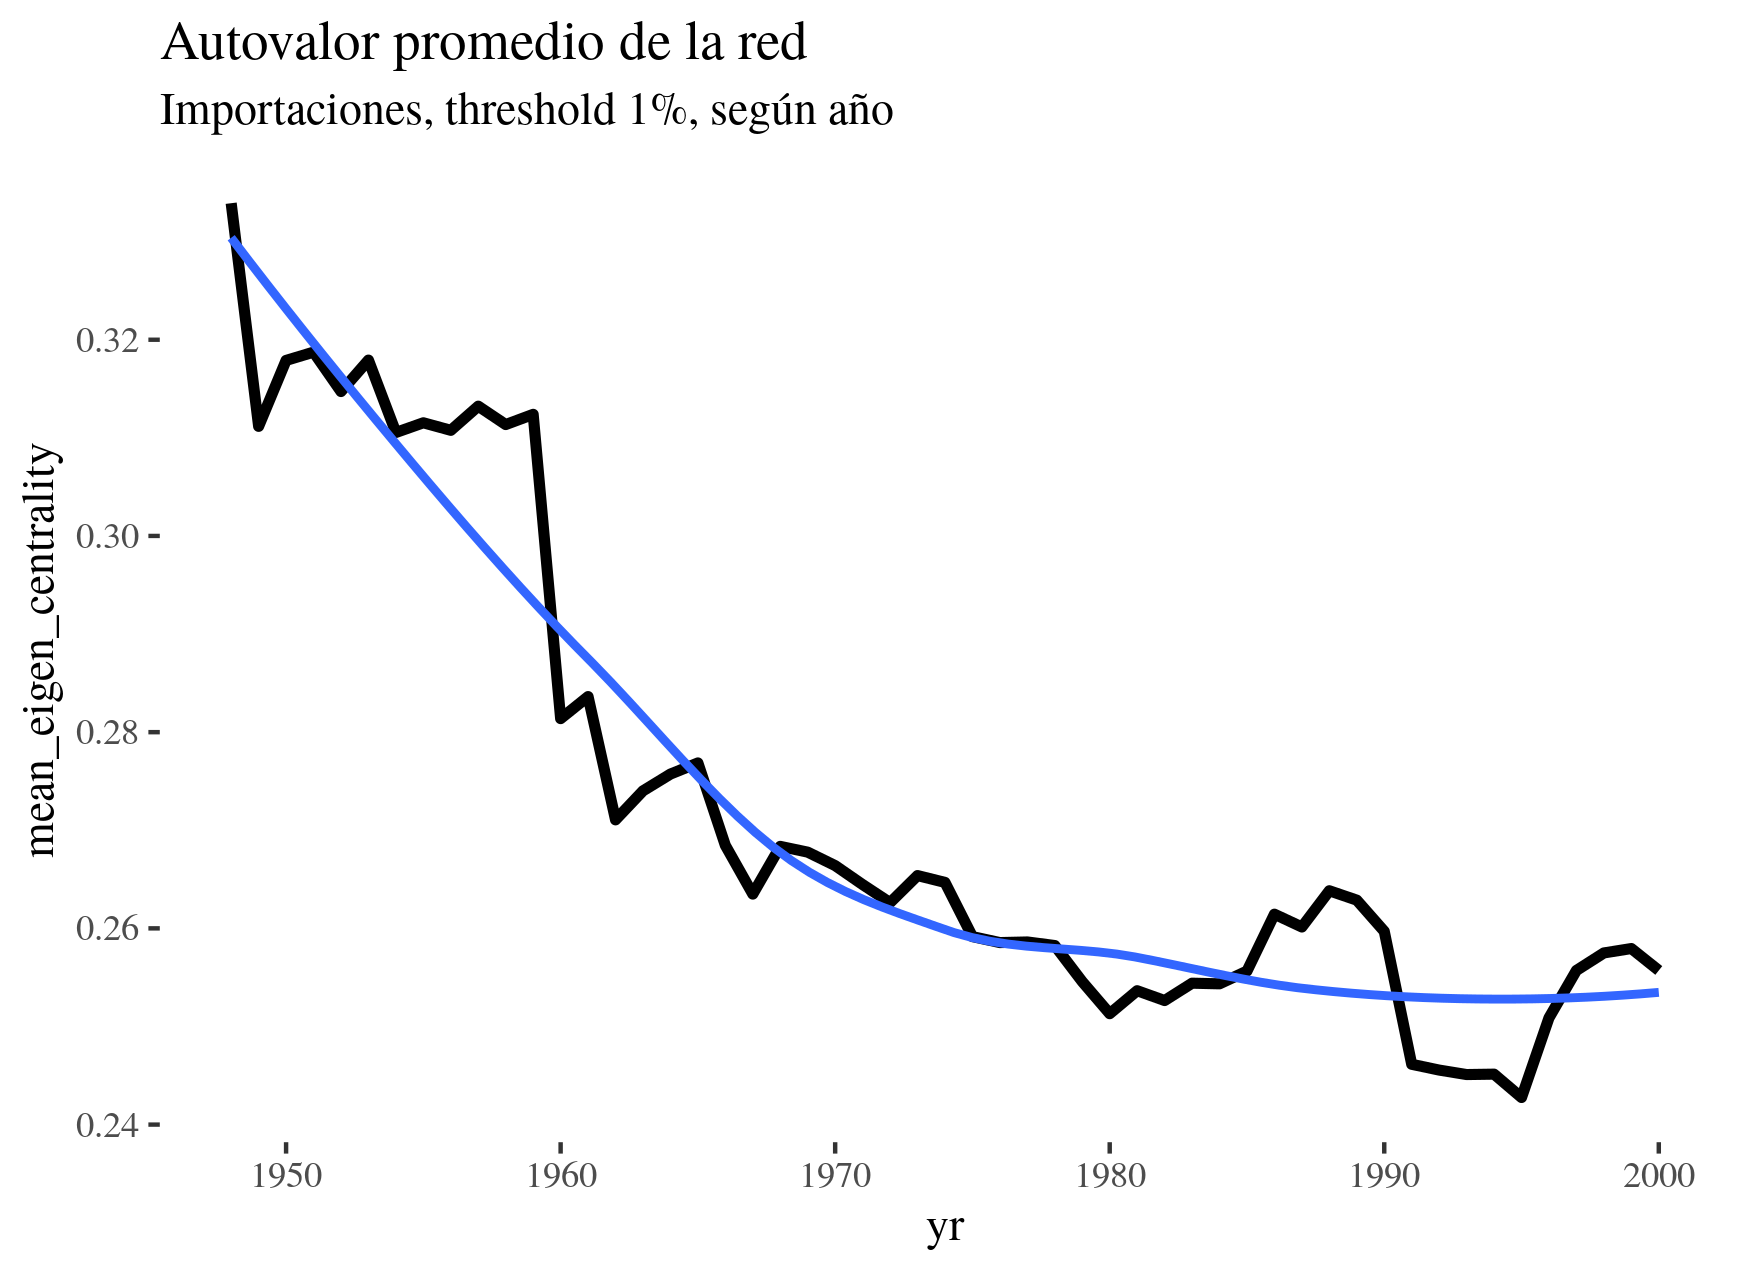
\includegraphics[width=.45\linewidth]{1950_2000_mean_eigen_centrality_x_yr}}
	\subfigure[Autovalor promedio. Ponderado por valor comercial]{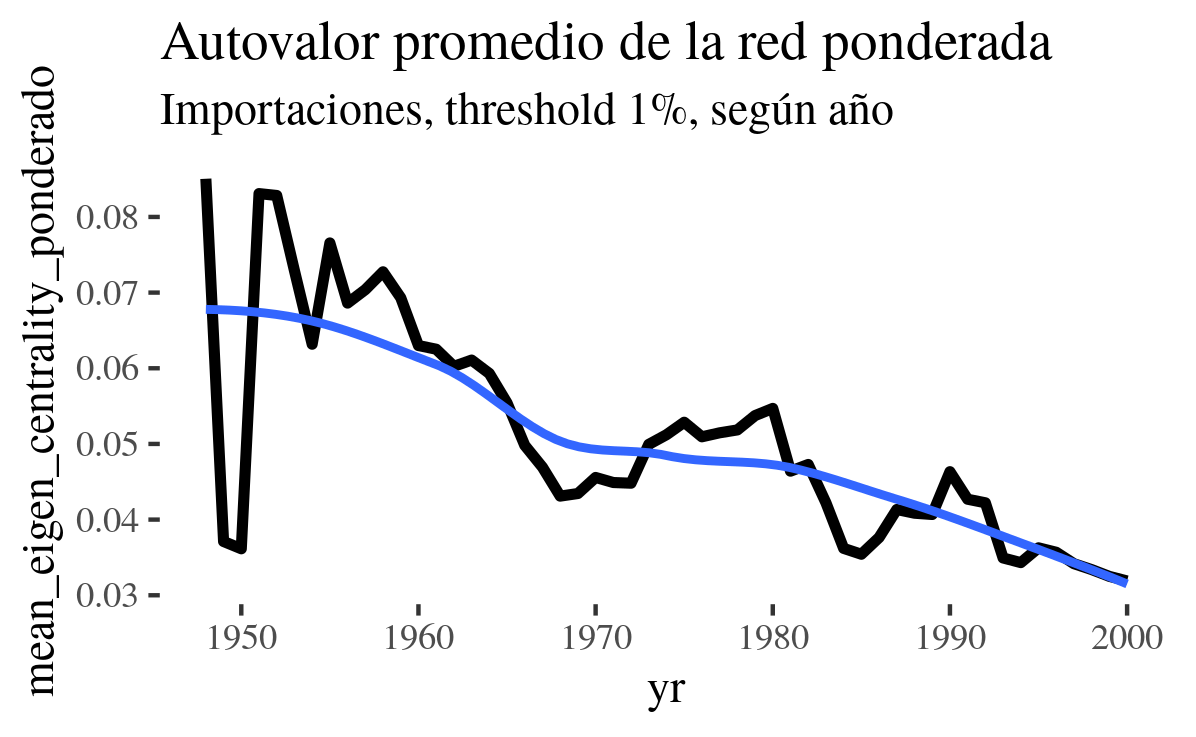
\includegraphics[width=.45\linewidth]{1950_2000_mean_eigen_centrality_ponderado_x_yr}}	
	\caption{Evolución de la estructura de la red. Importaciones. Umbral 1\%.1948-2000}
	\label{fig:metricas_LP_comp}
\end{figure}


\begin{figure}
	\centering
	\subfigure[1966]{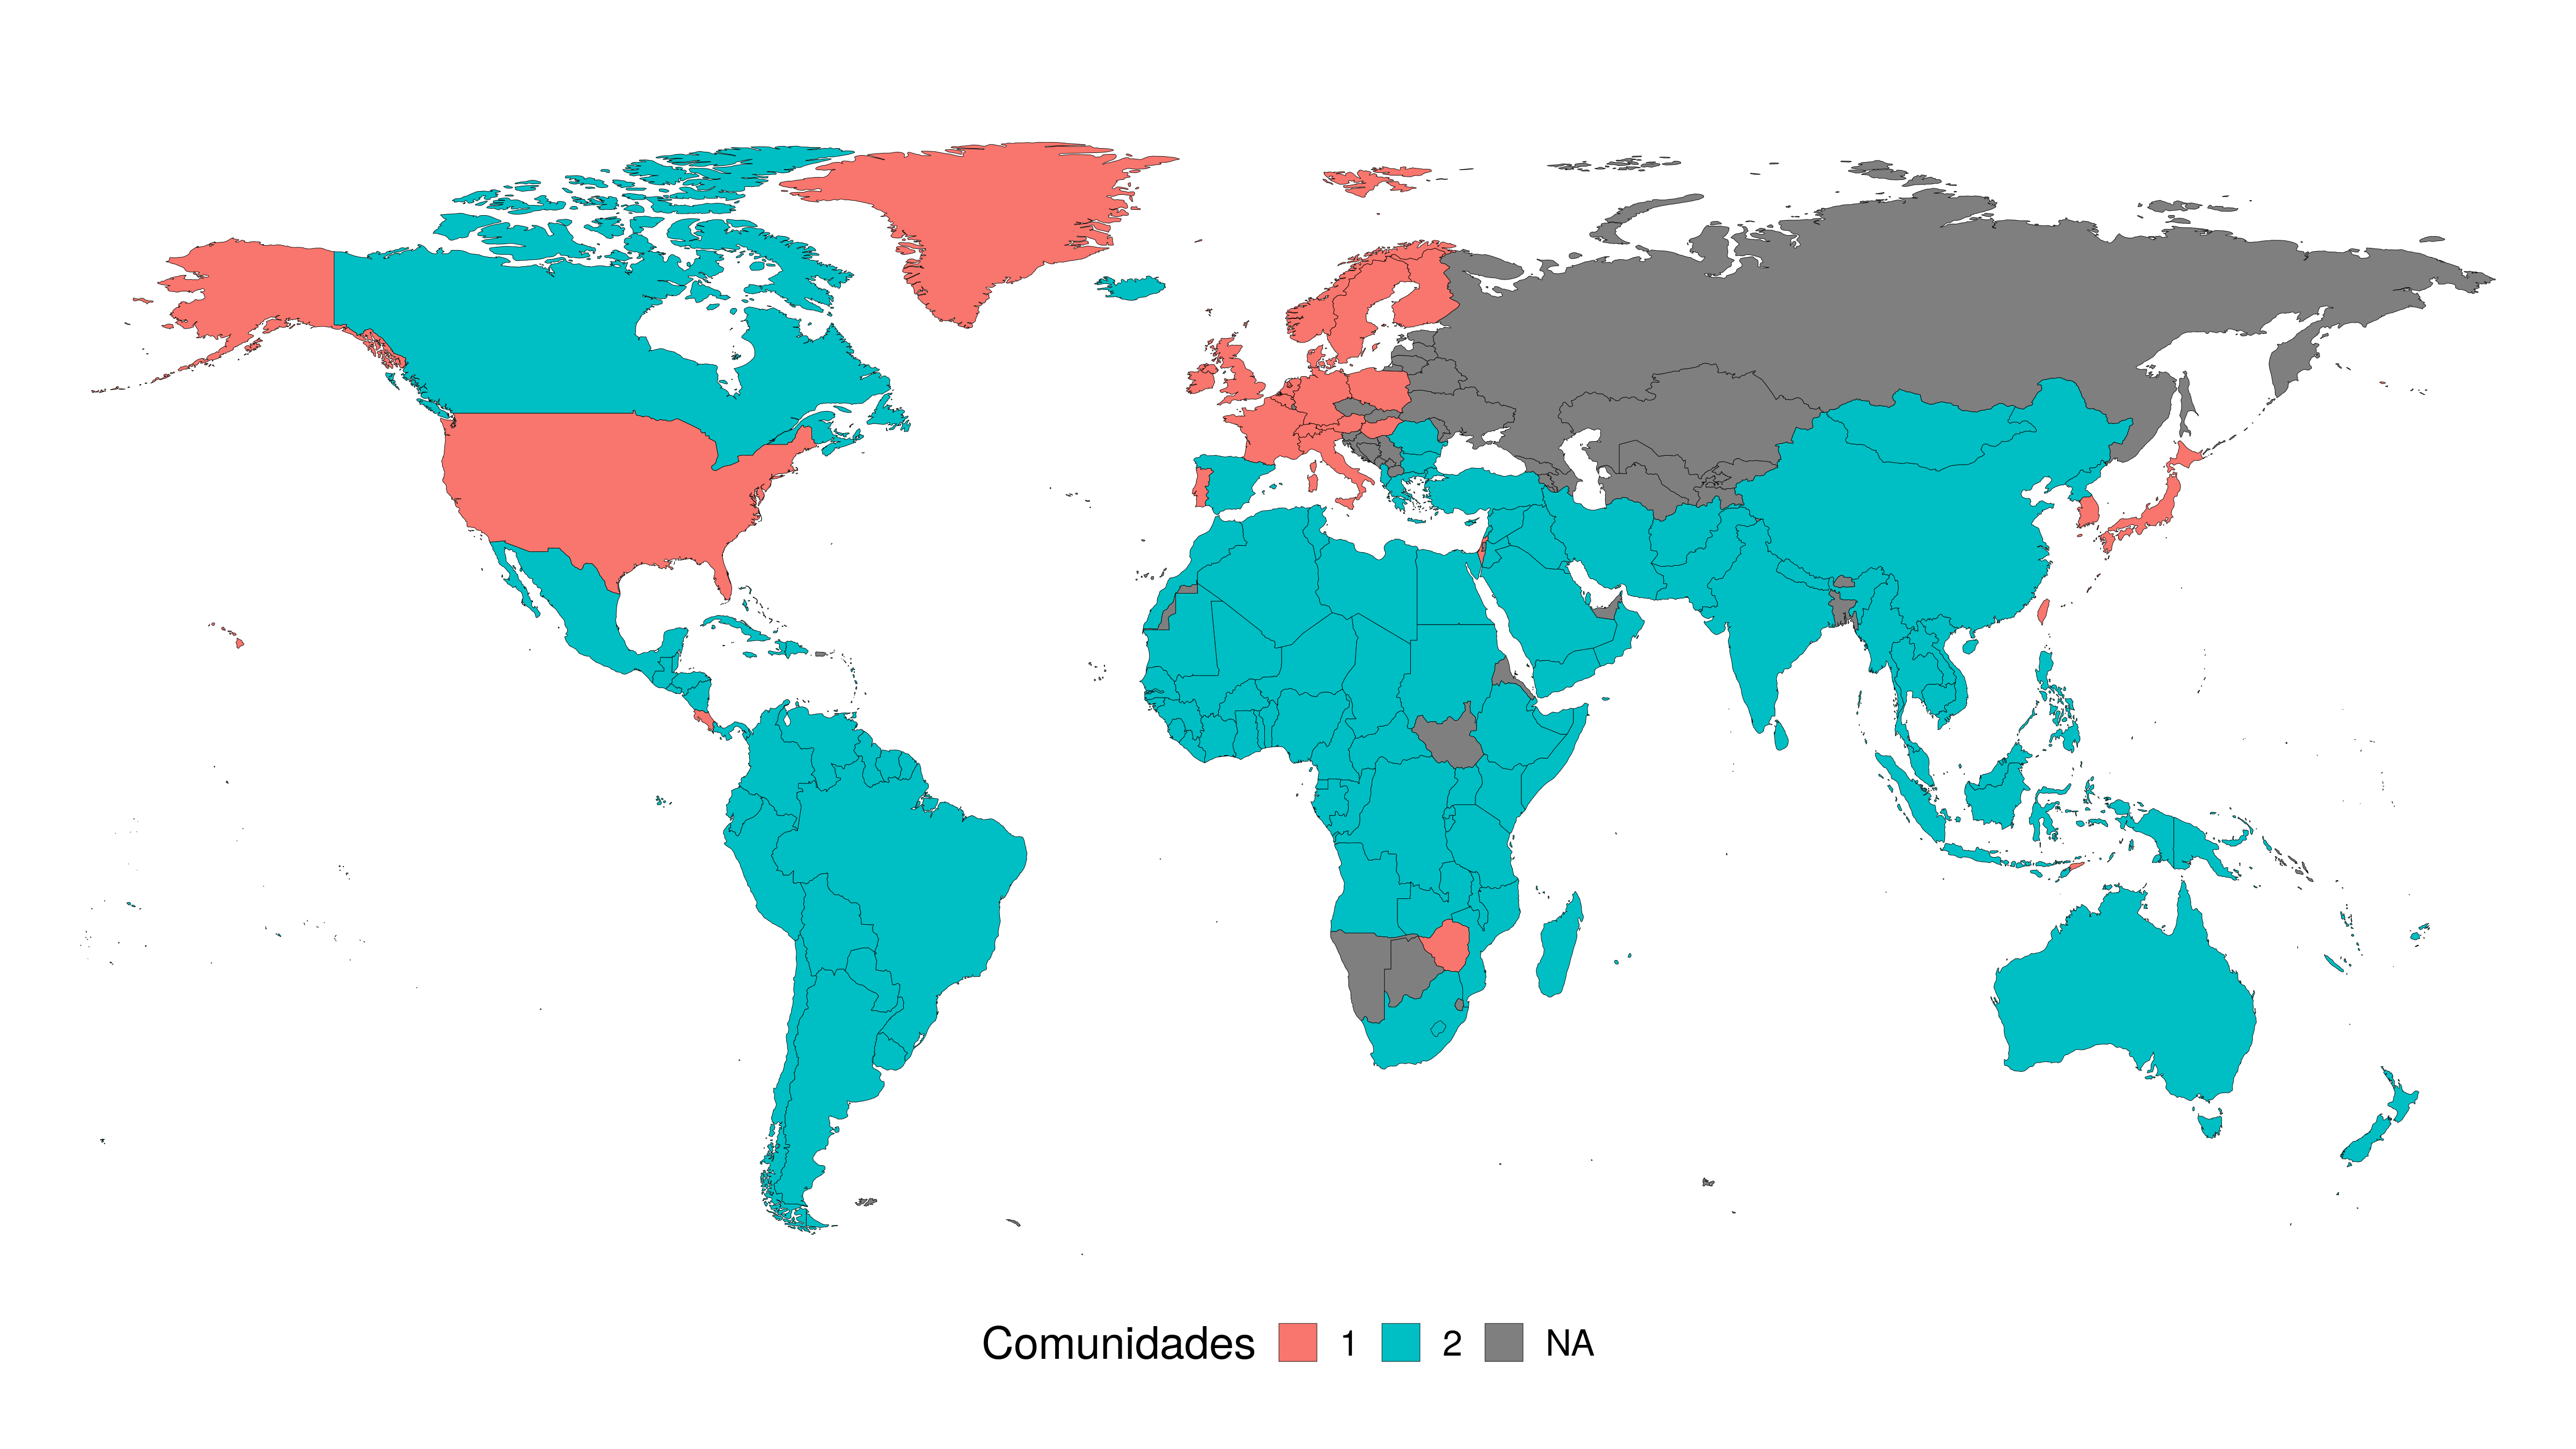
\includegraphics[width=0.45\linewidth]{mapa_projection_walktrap_lp_1966}}
	\subfigure[1976]{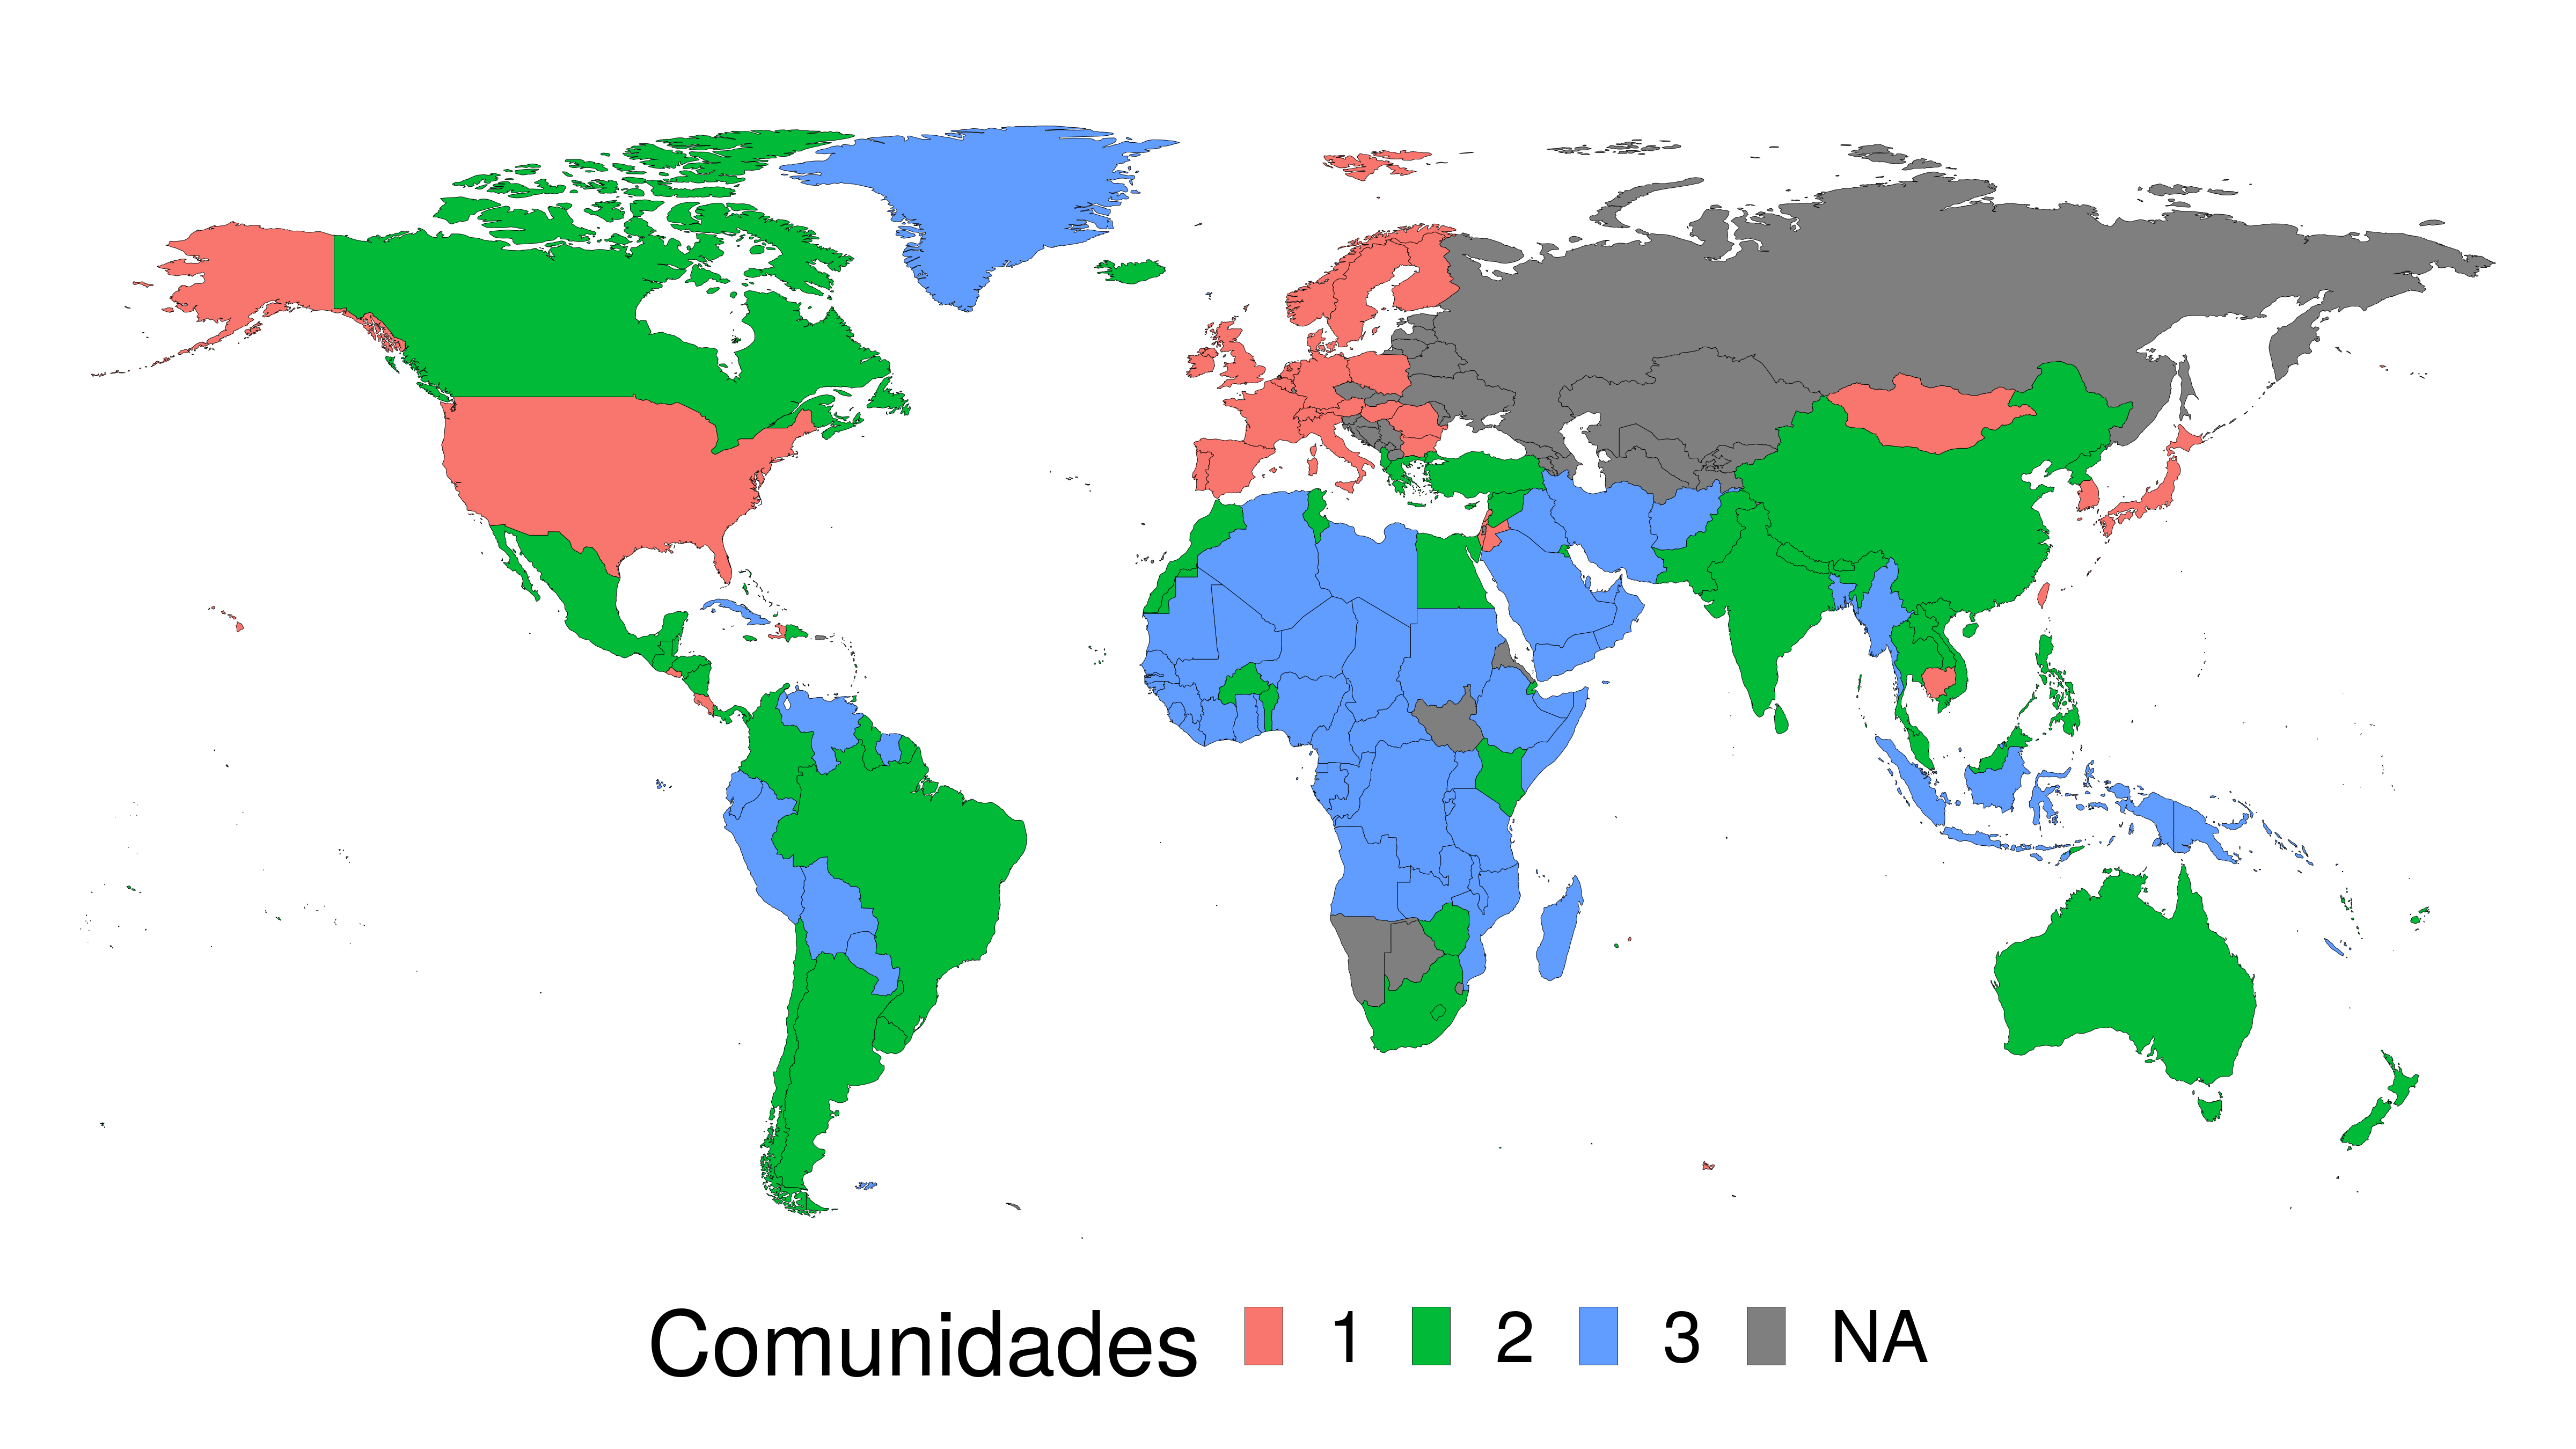
\includegraphics[width=0.45\linewidth]{mapa_projection_walktrap_lp_1976}}
	\subfigure[1986]{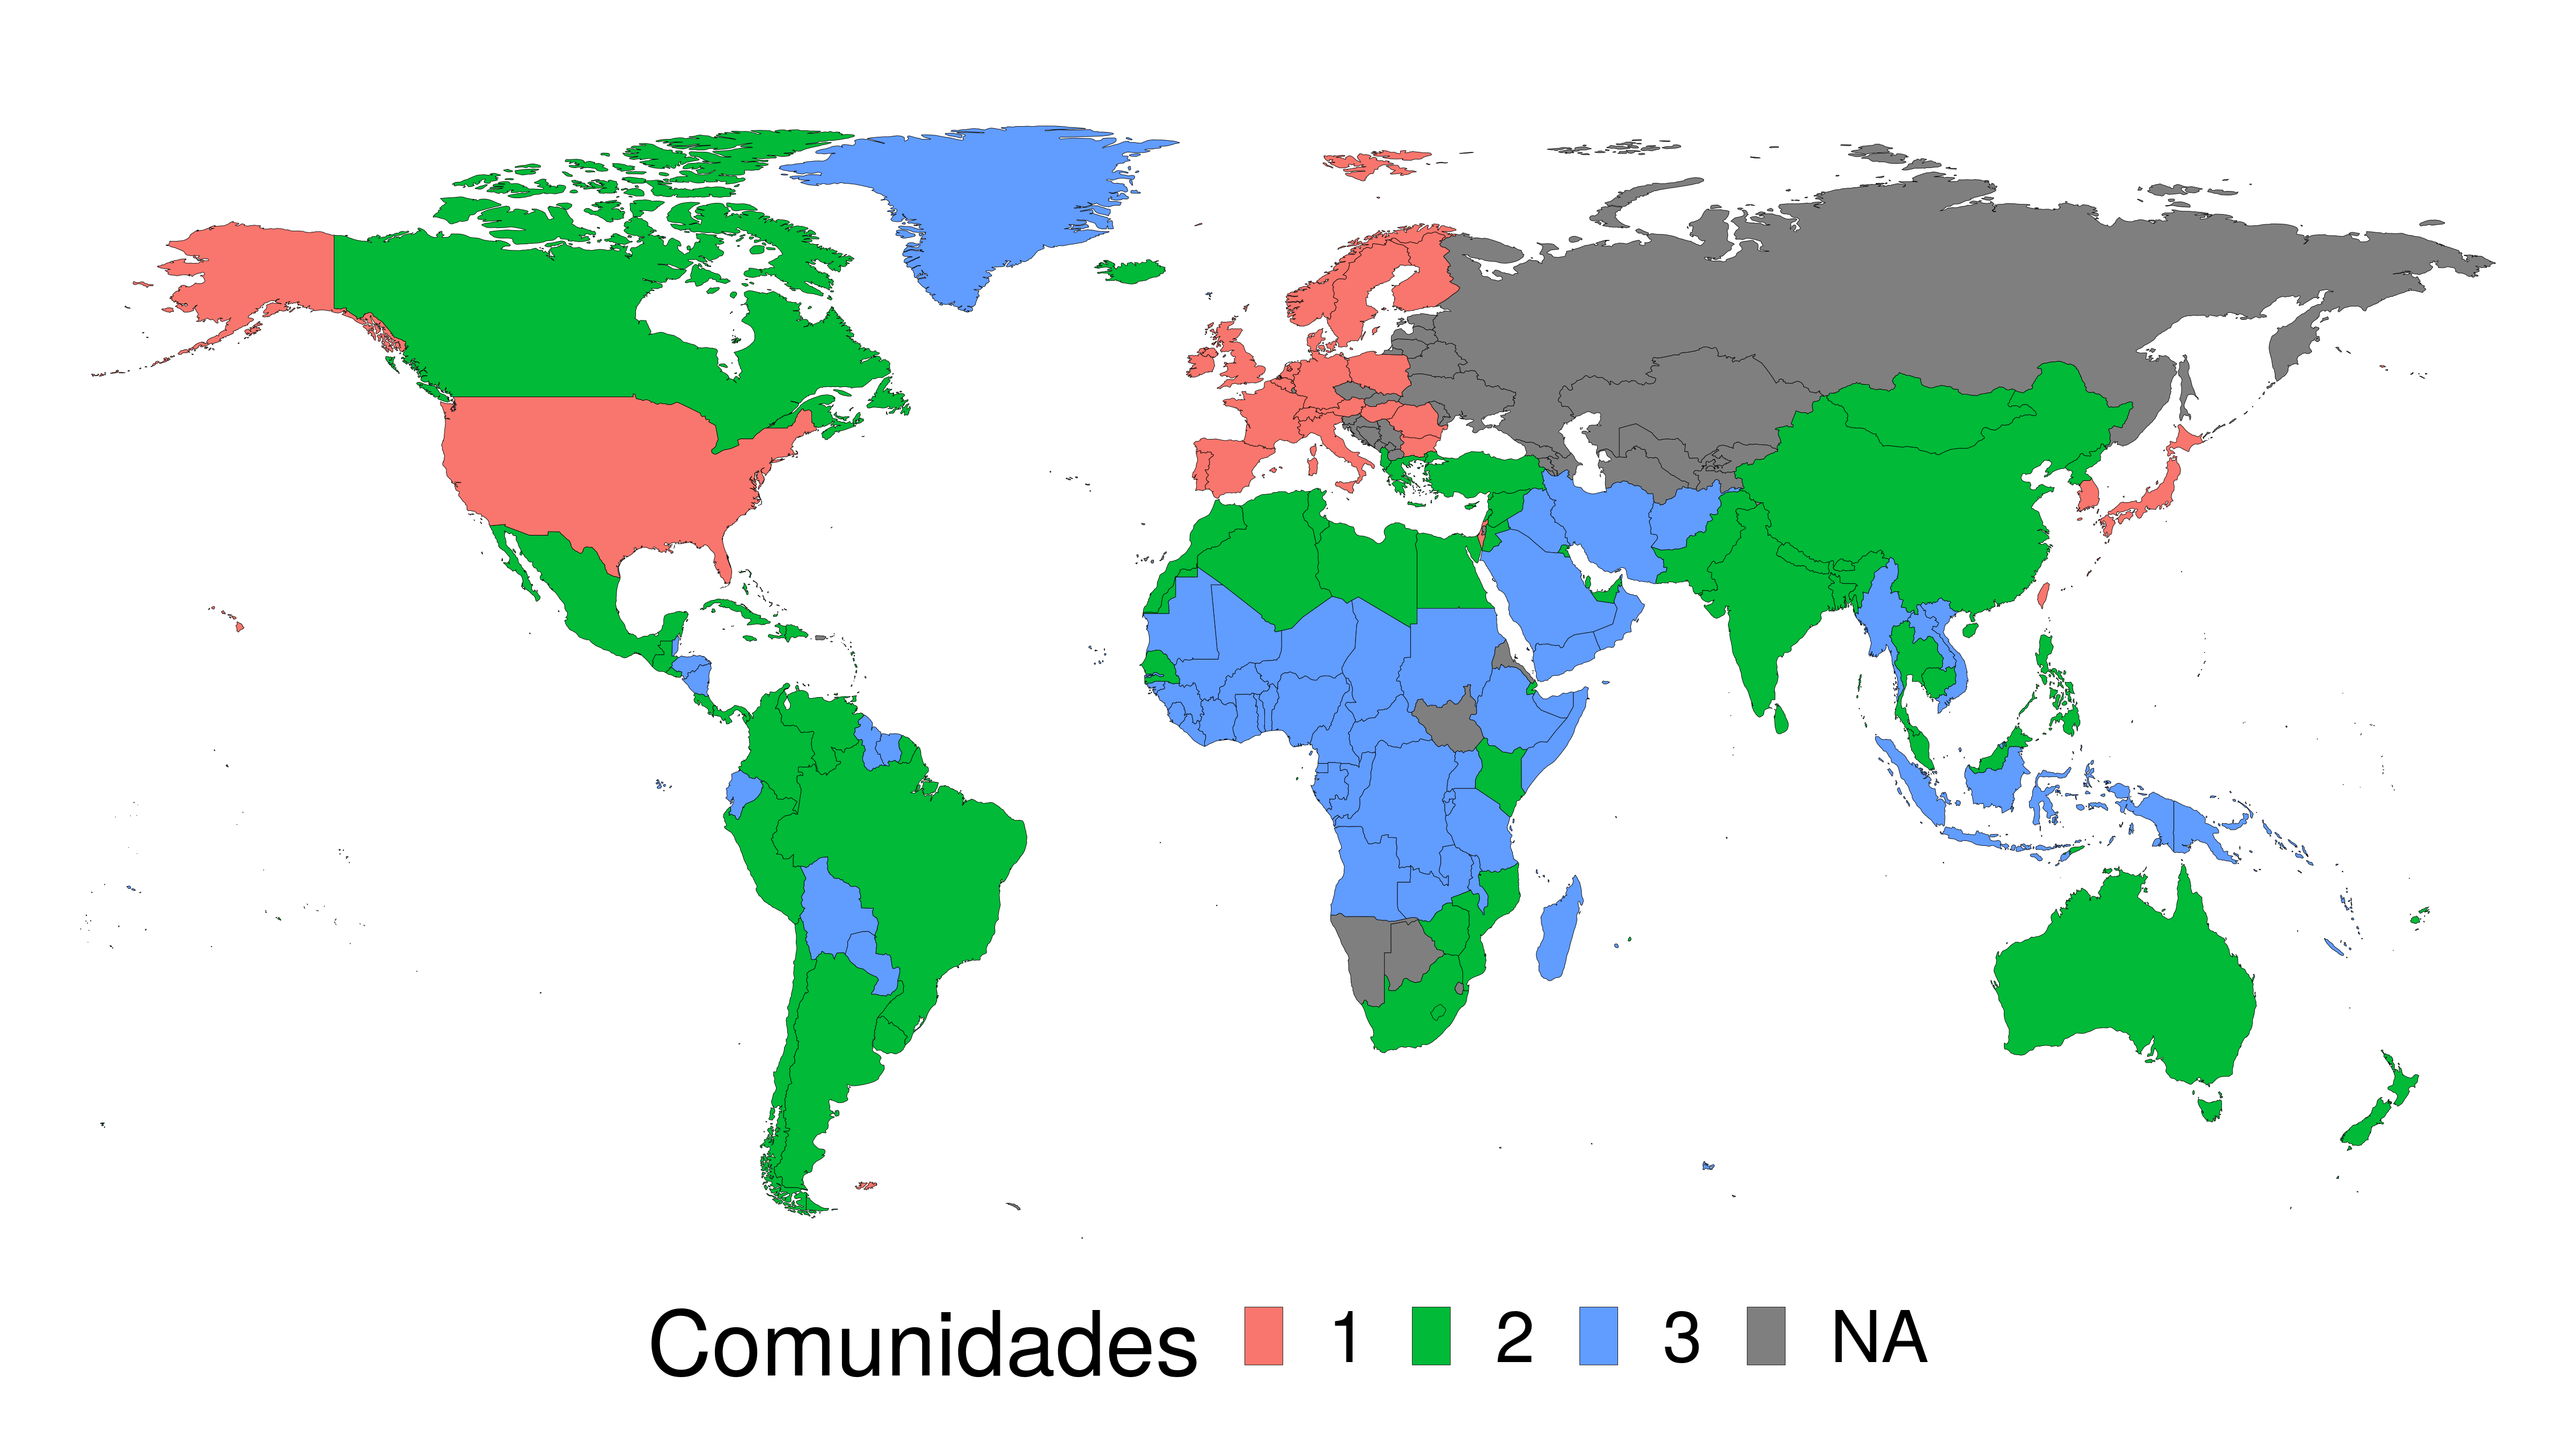
\includegraphics[width=0.45\linewidth]{mapa_projection_walktrap_lp_1986}}
	\subfigure[1996]{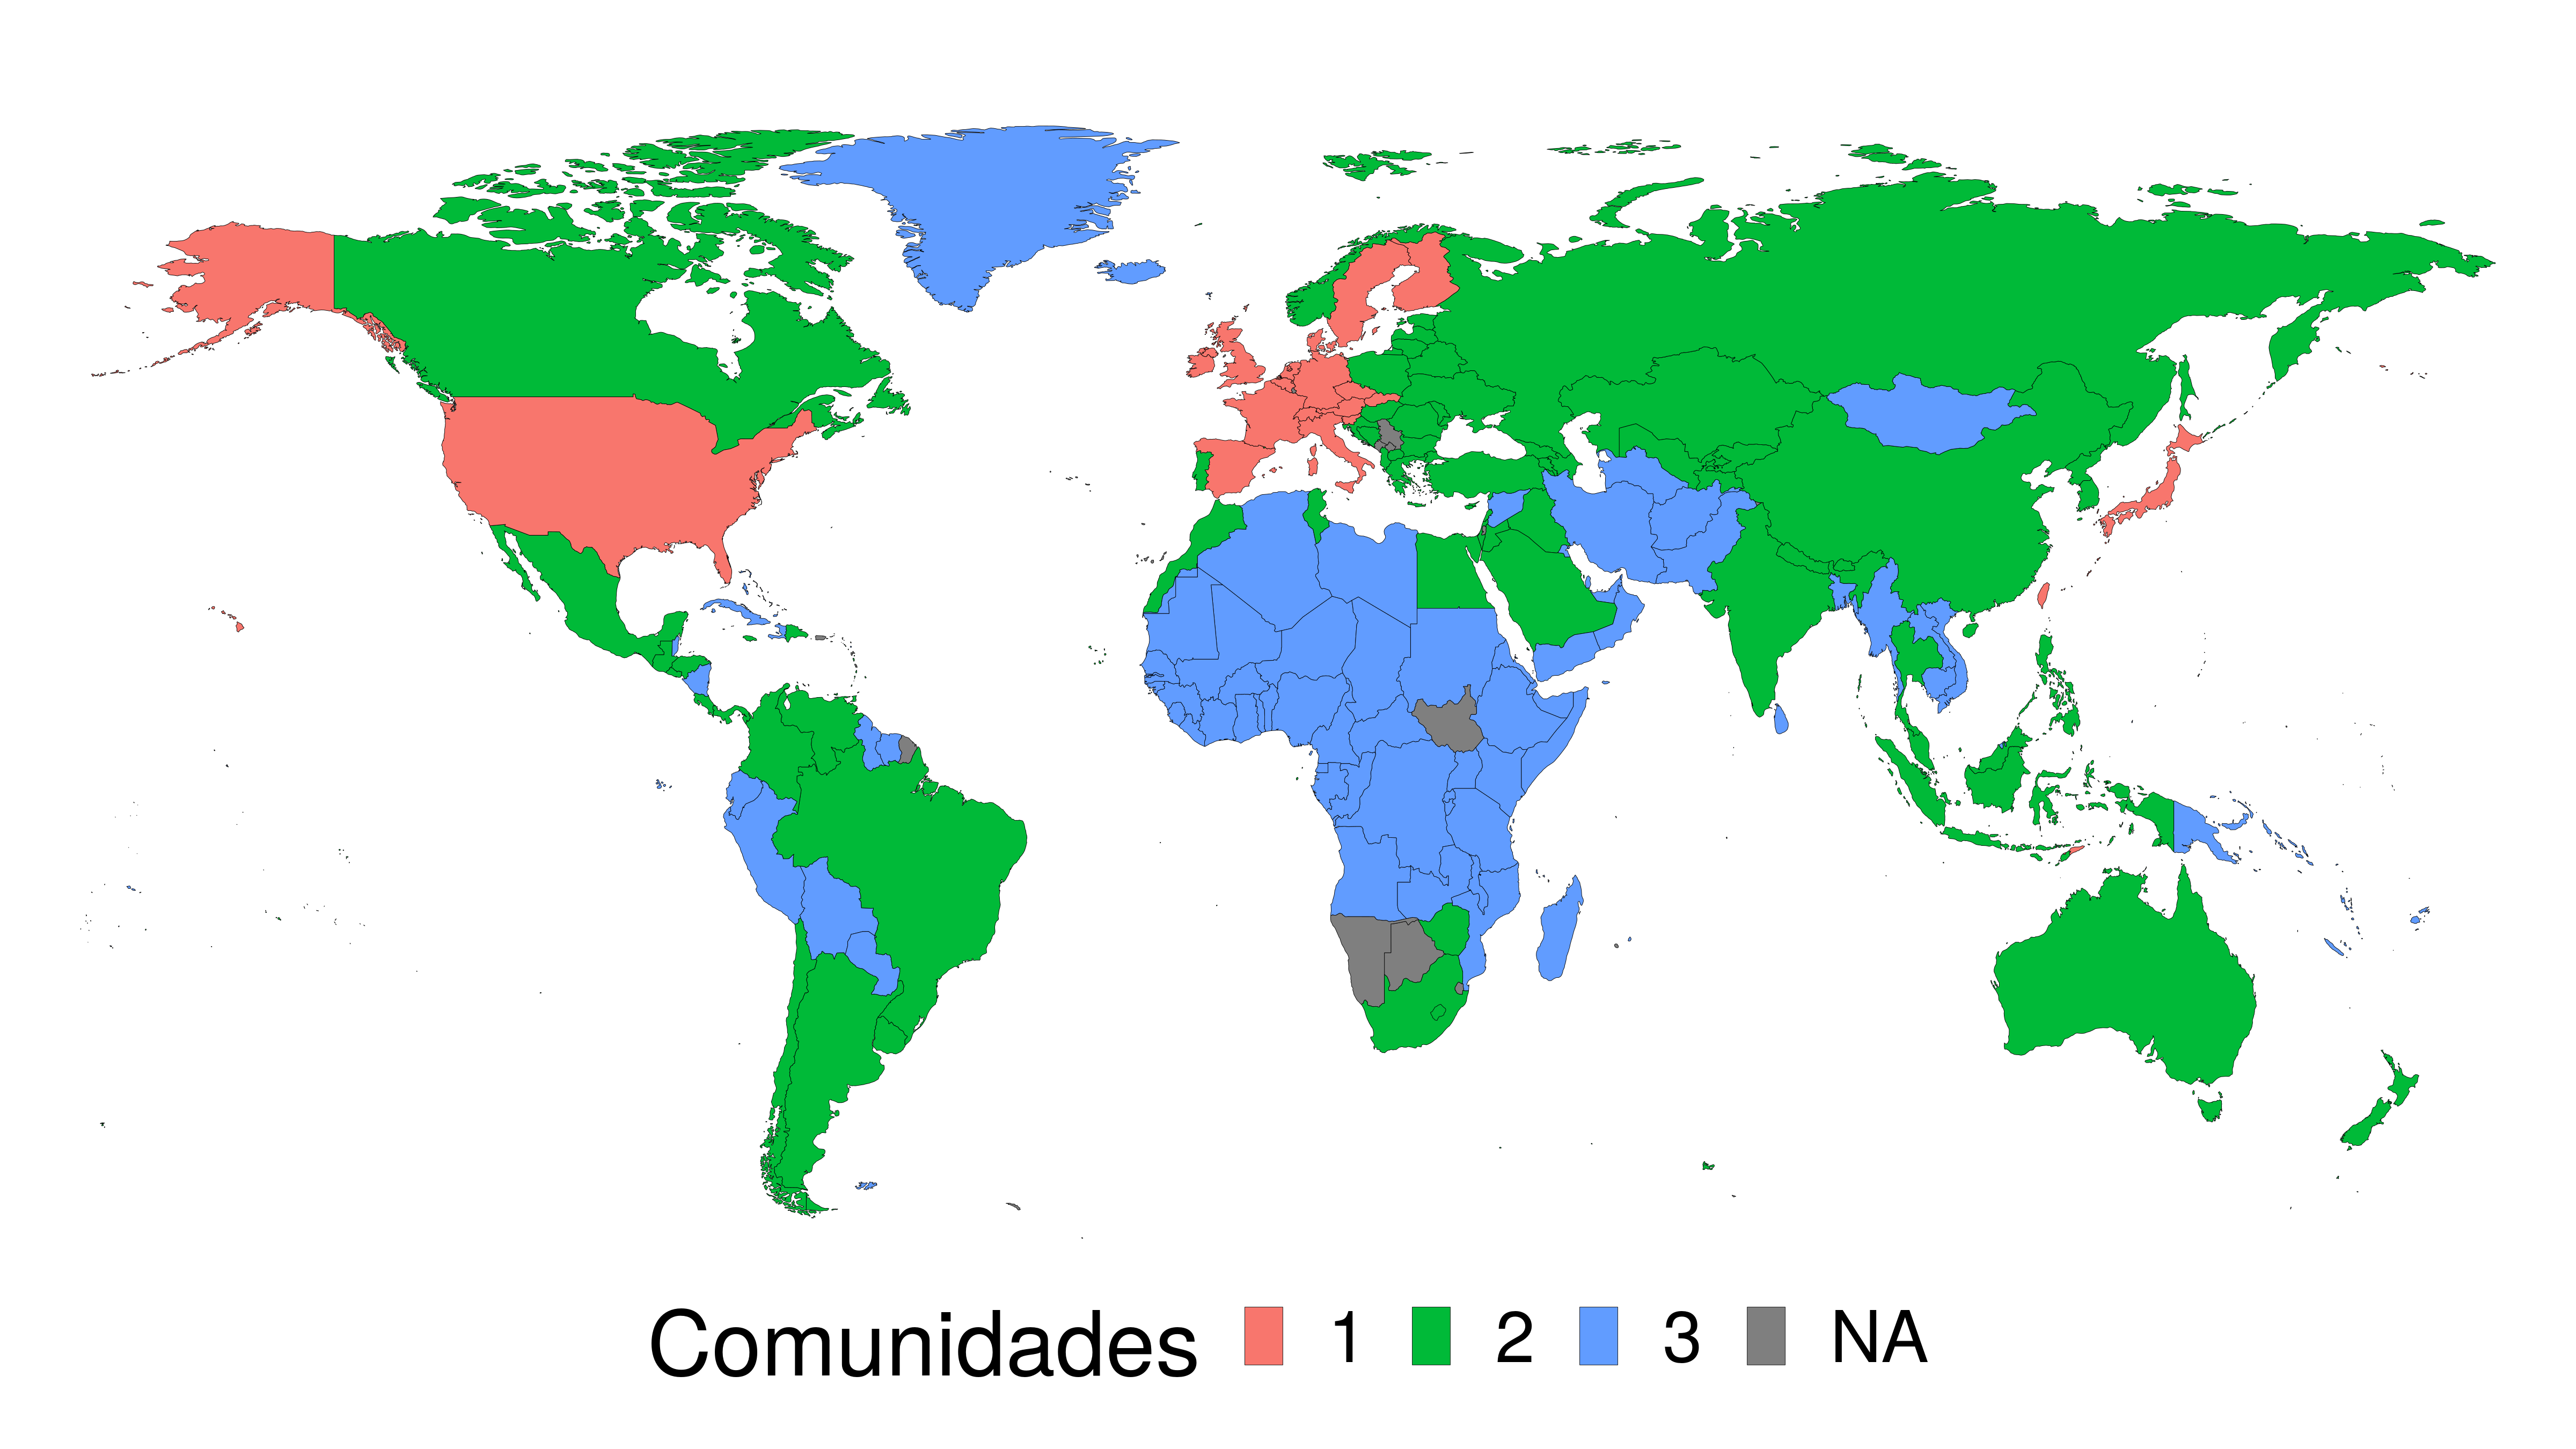
\includegraphics[width=0.45\linewidth]{mapa_projection_walktrap_lp_1996}}
	\subfigure[2016]{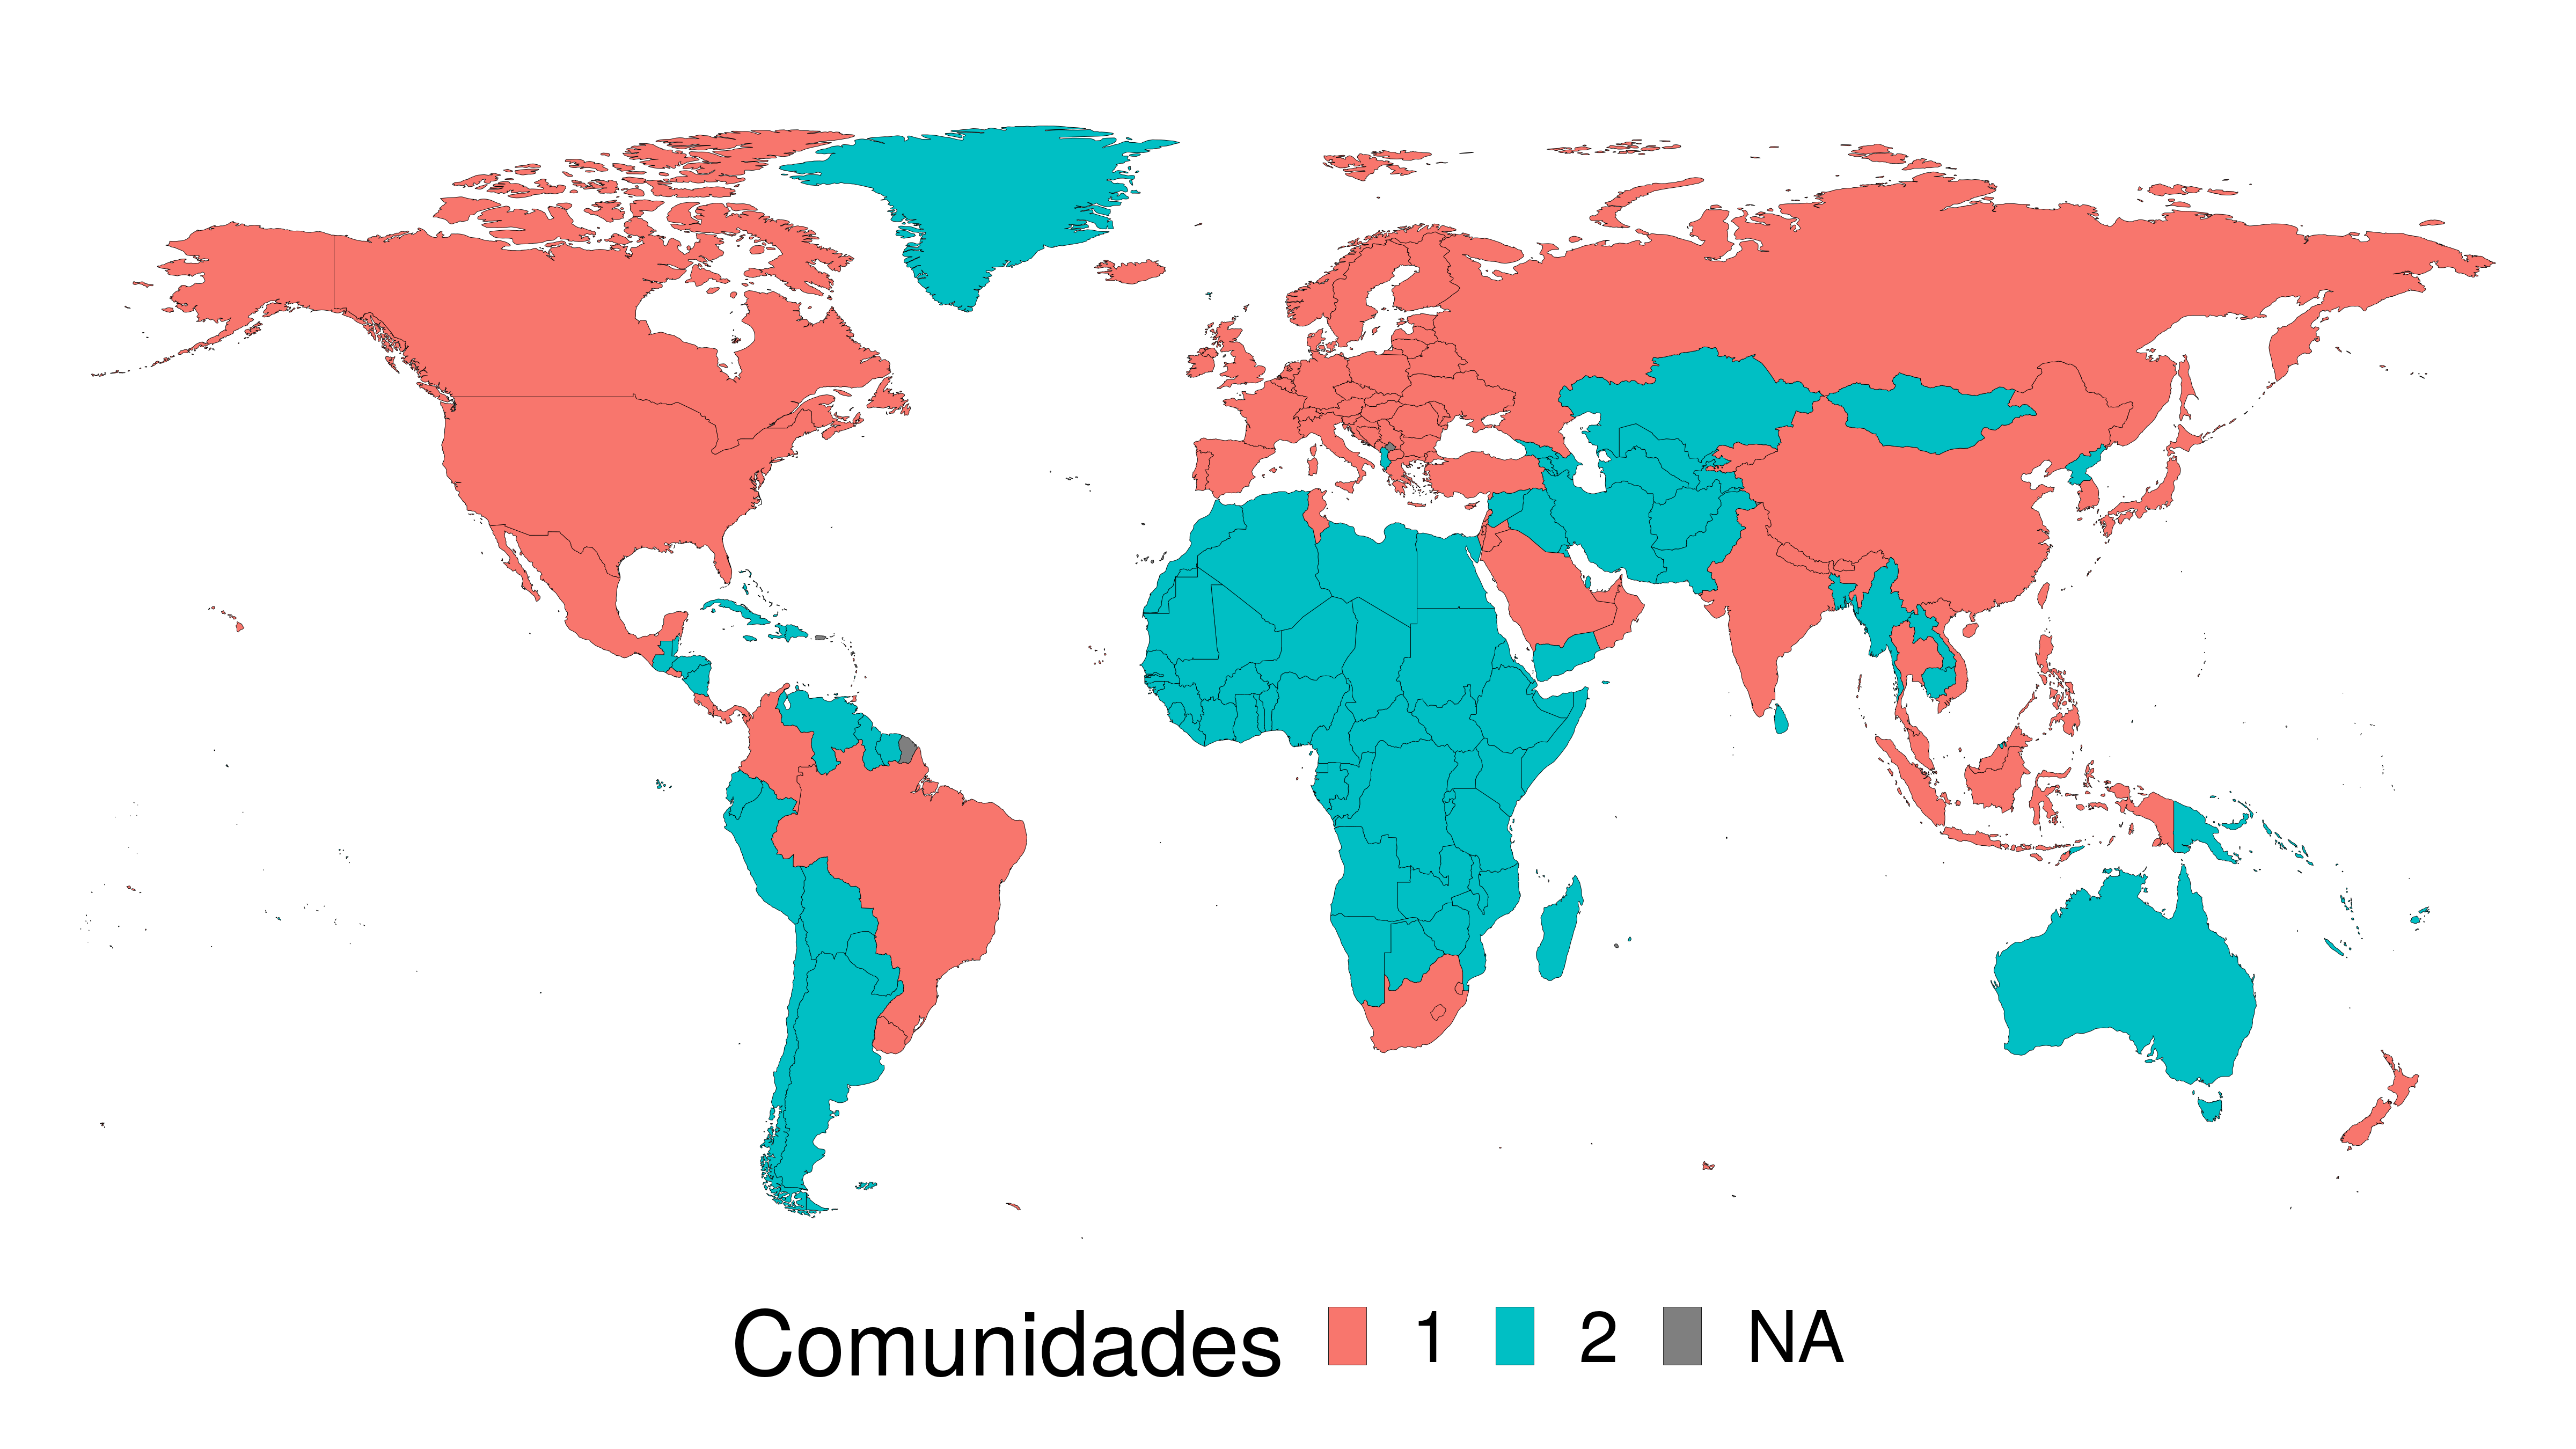
\includegraphics[width=0.5\linewidth]{mapa_projection_walktrap_lp_2016}}
	\caption{Proyección a países del grafo bipartito. Clustering Walktrap. Exportaciones}
	\label{fig:mapas_proyeccion_walktrap}
\end{figure}

\begin{figure}
	\centering
	\subfigure[1966]{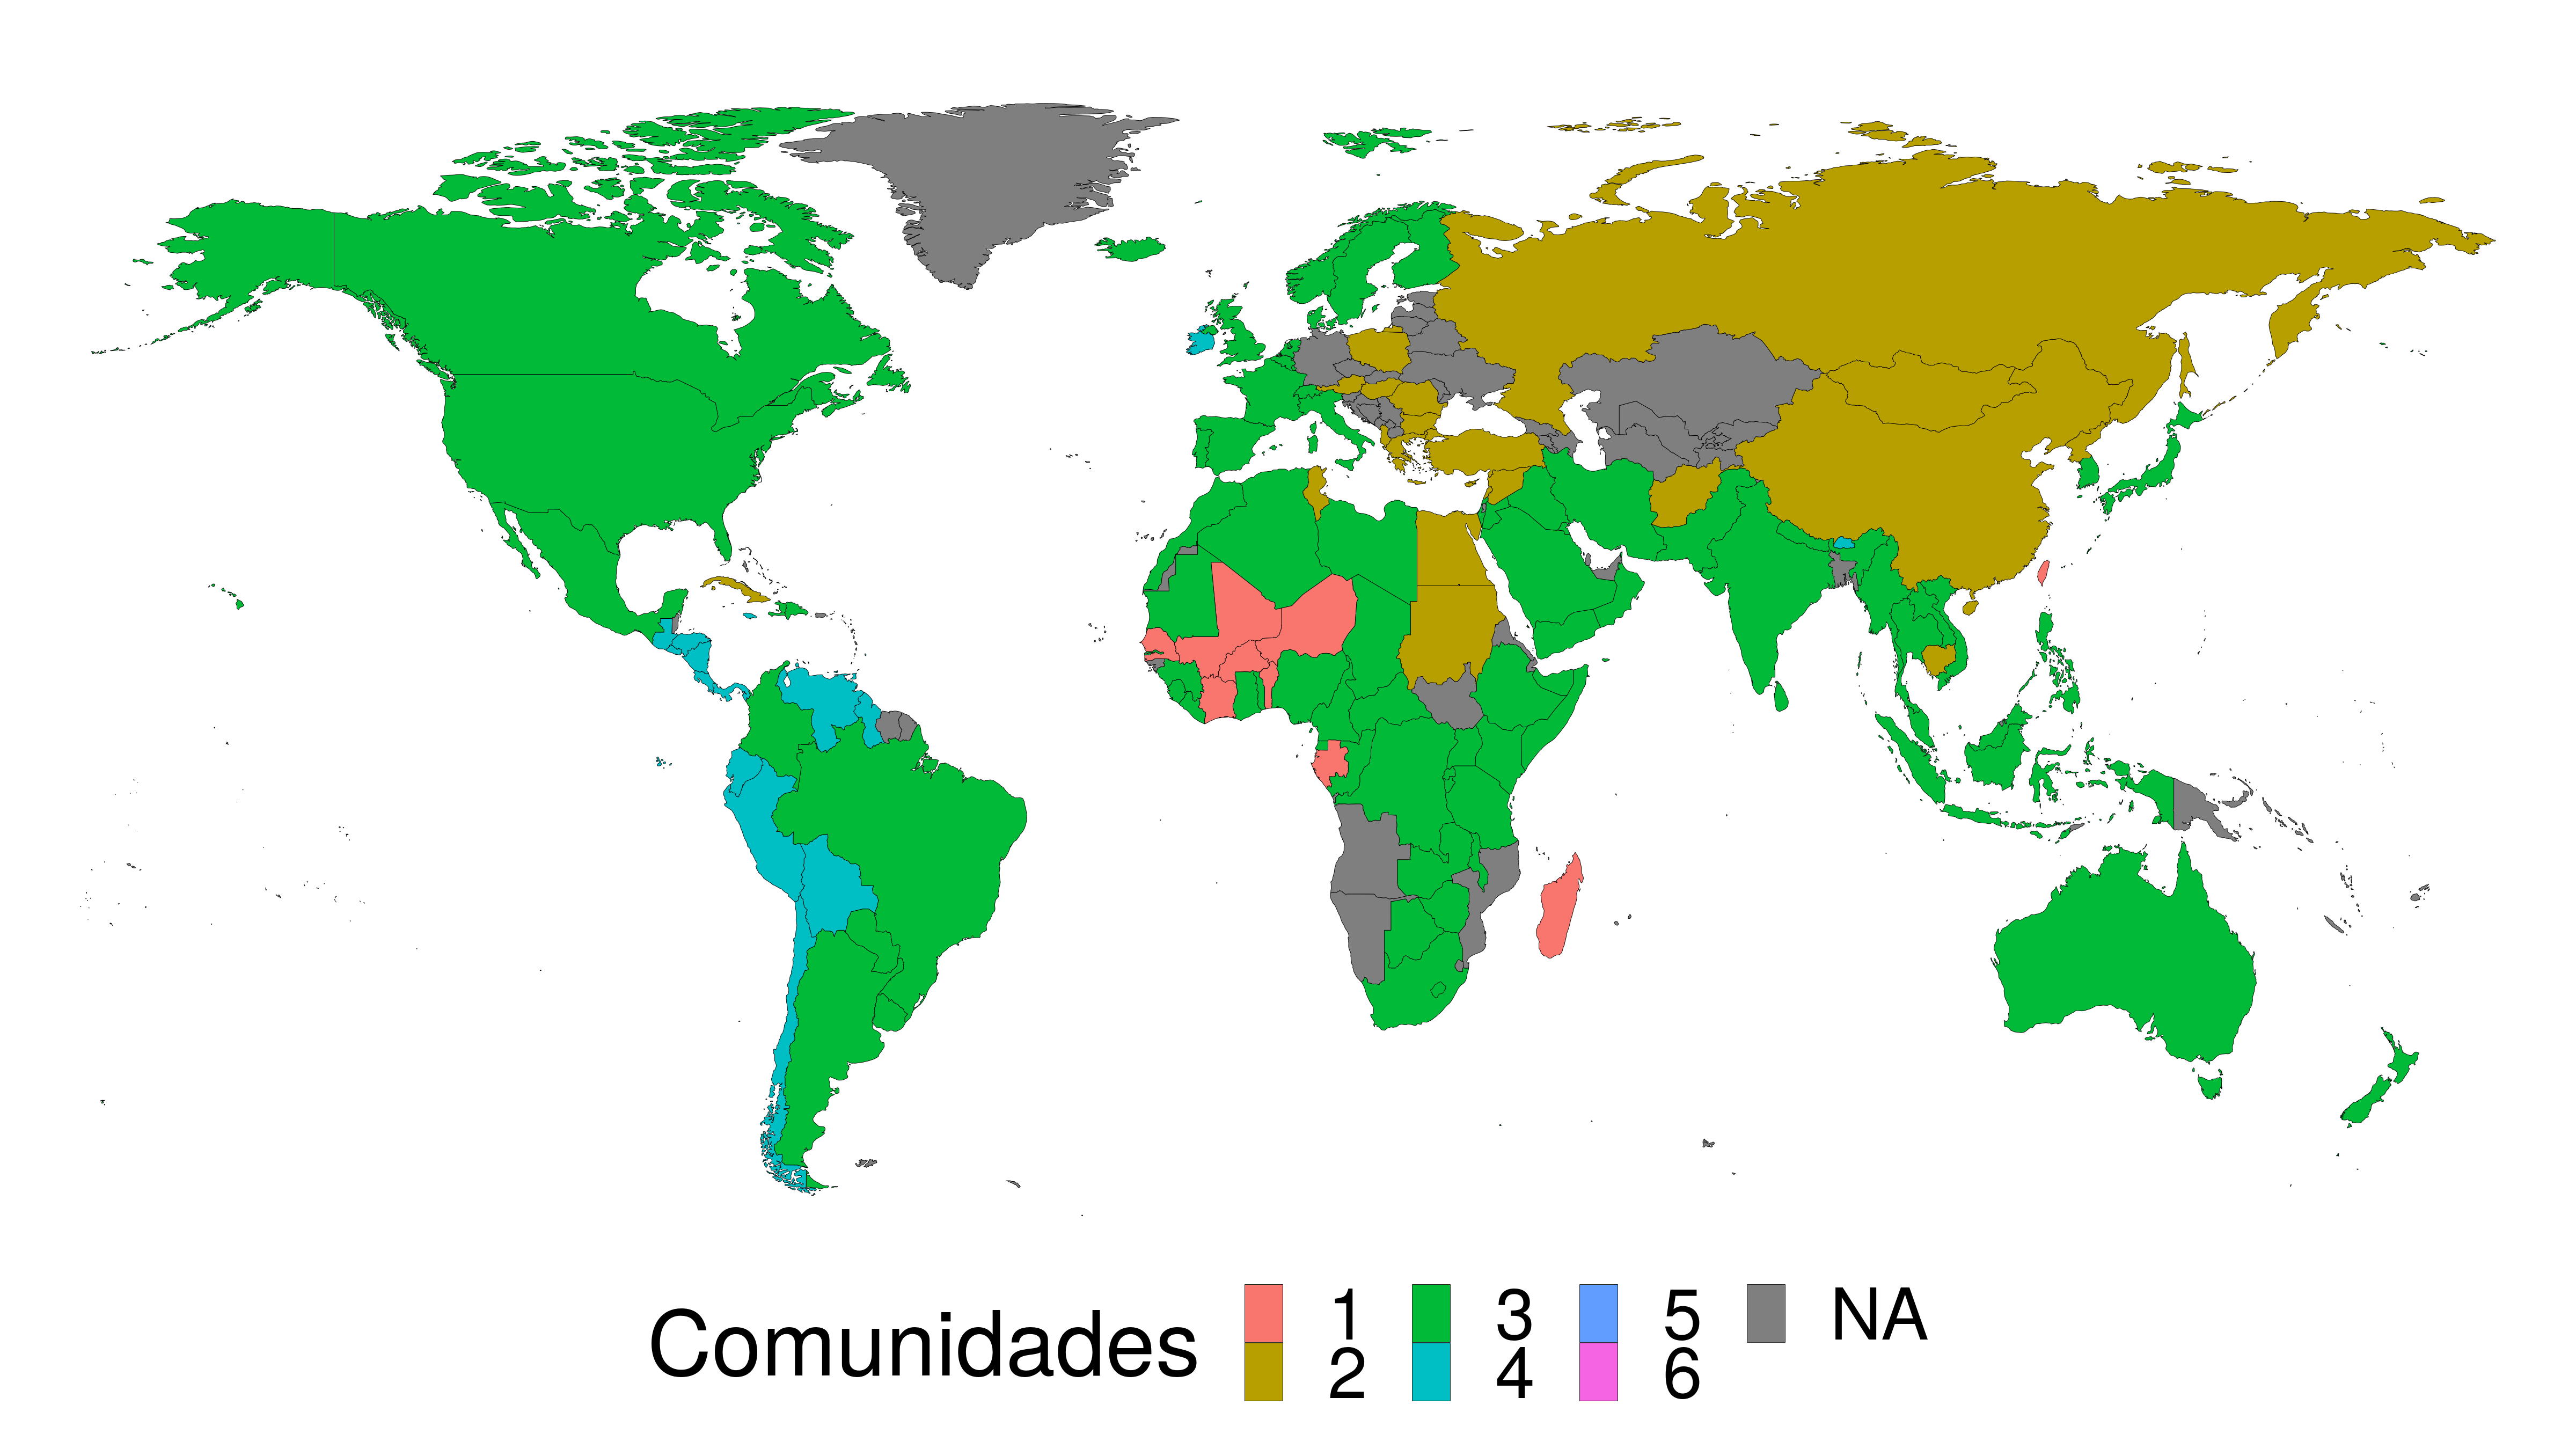
\includegraphics[width=0.45\linewidth]{mapa_walktrap_lp_1966}}
	\subfigure[1976]{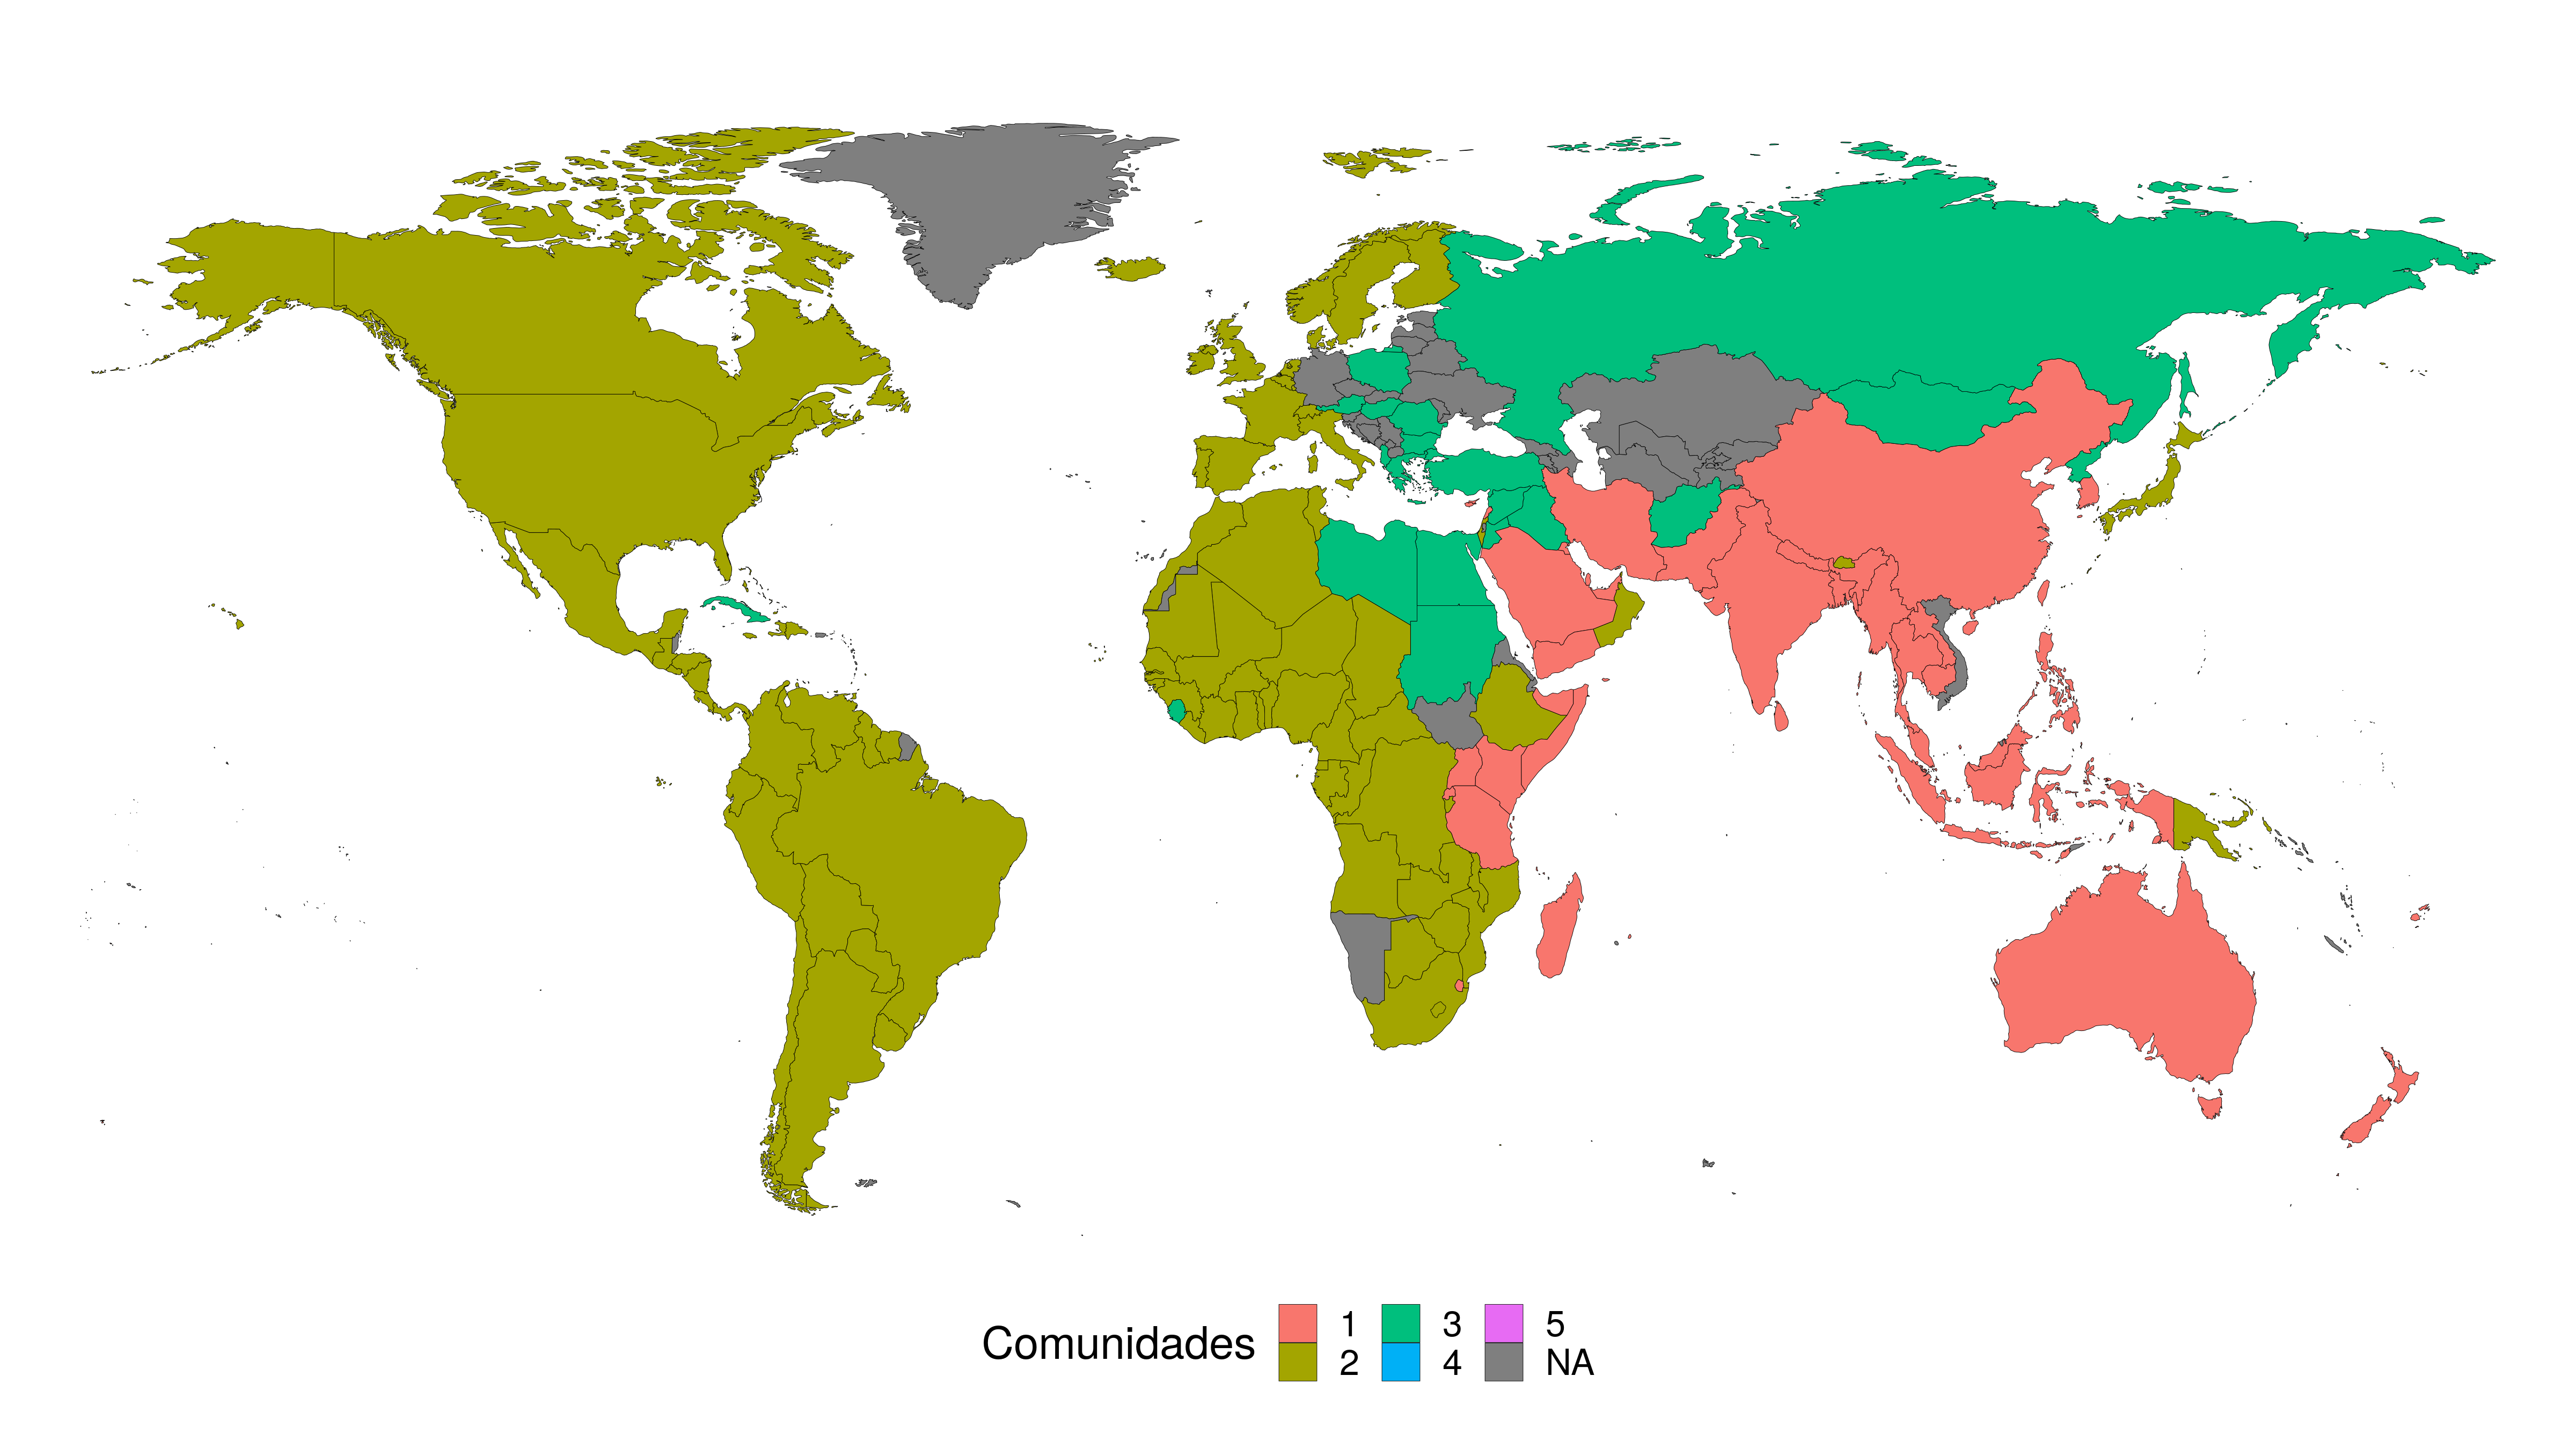
\includegraphics[width=0.45\linewidth]{mapa_walktrap_lp_1976}}
	\subfigure[1986]{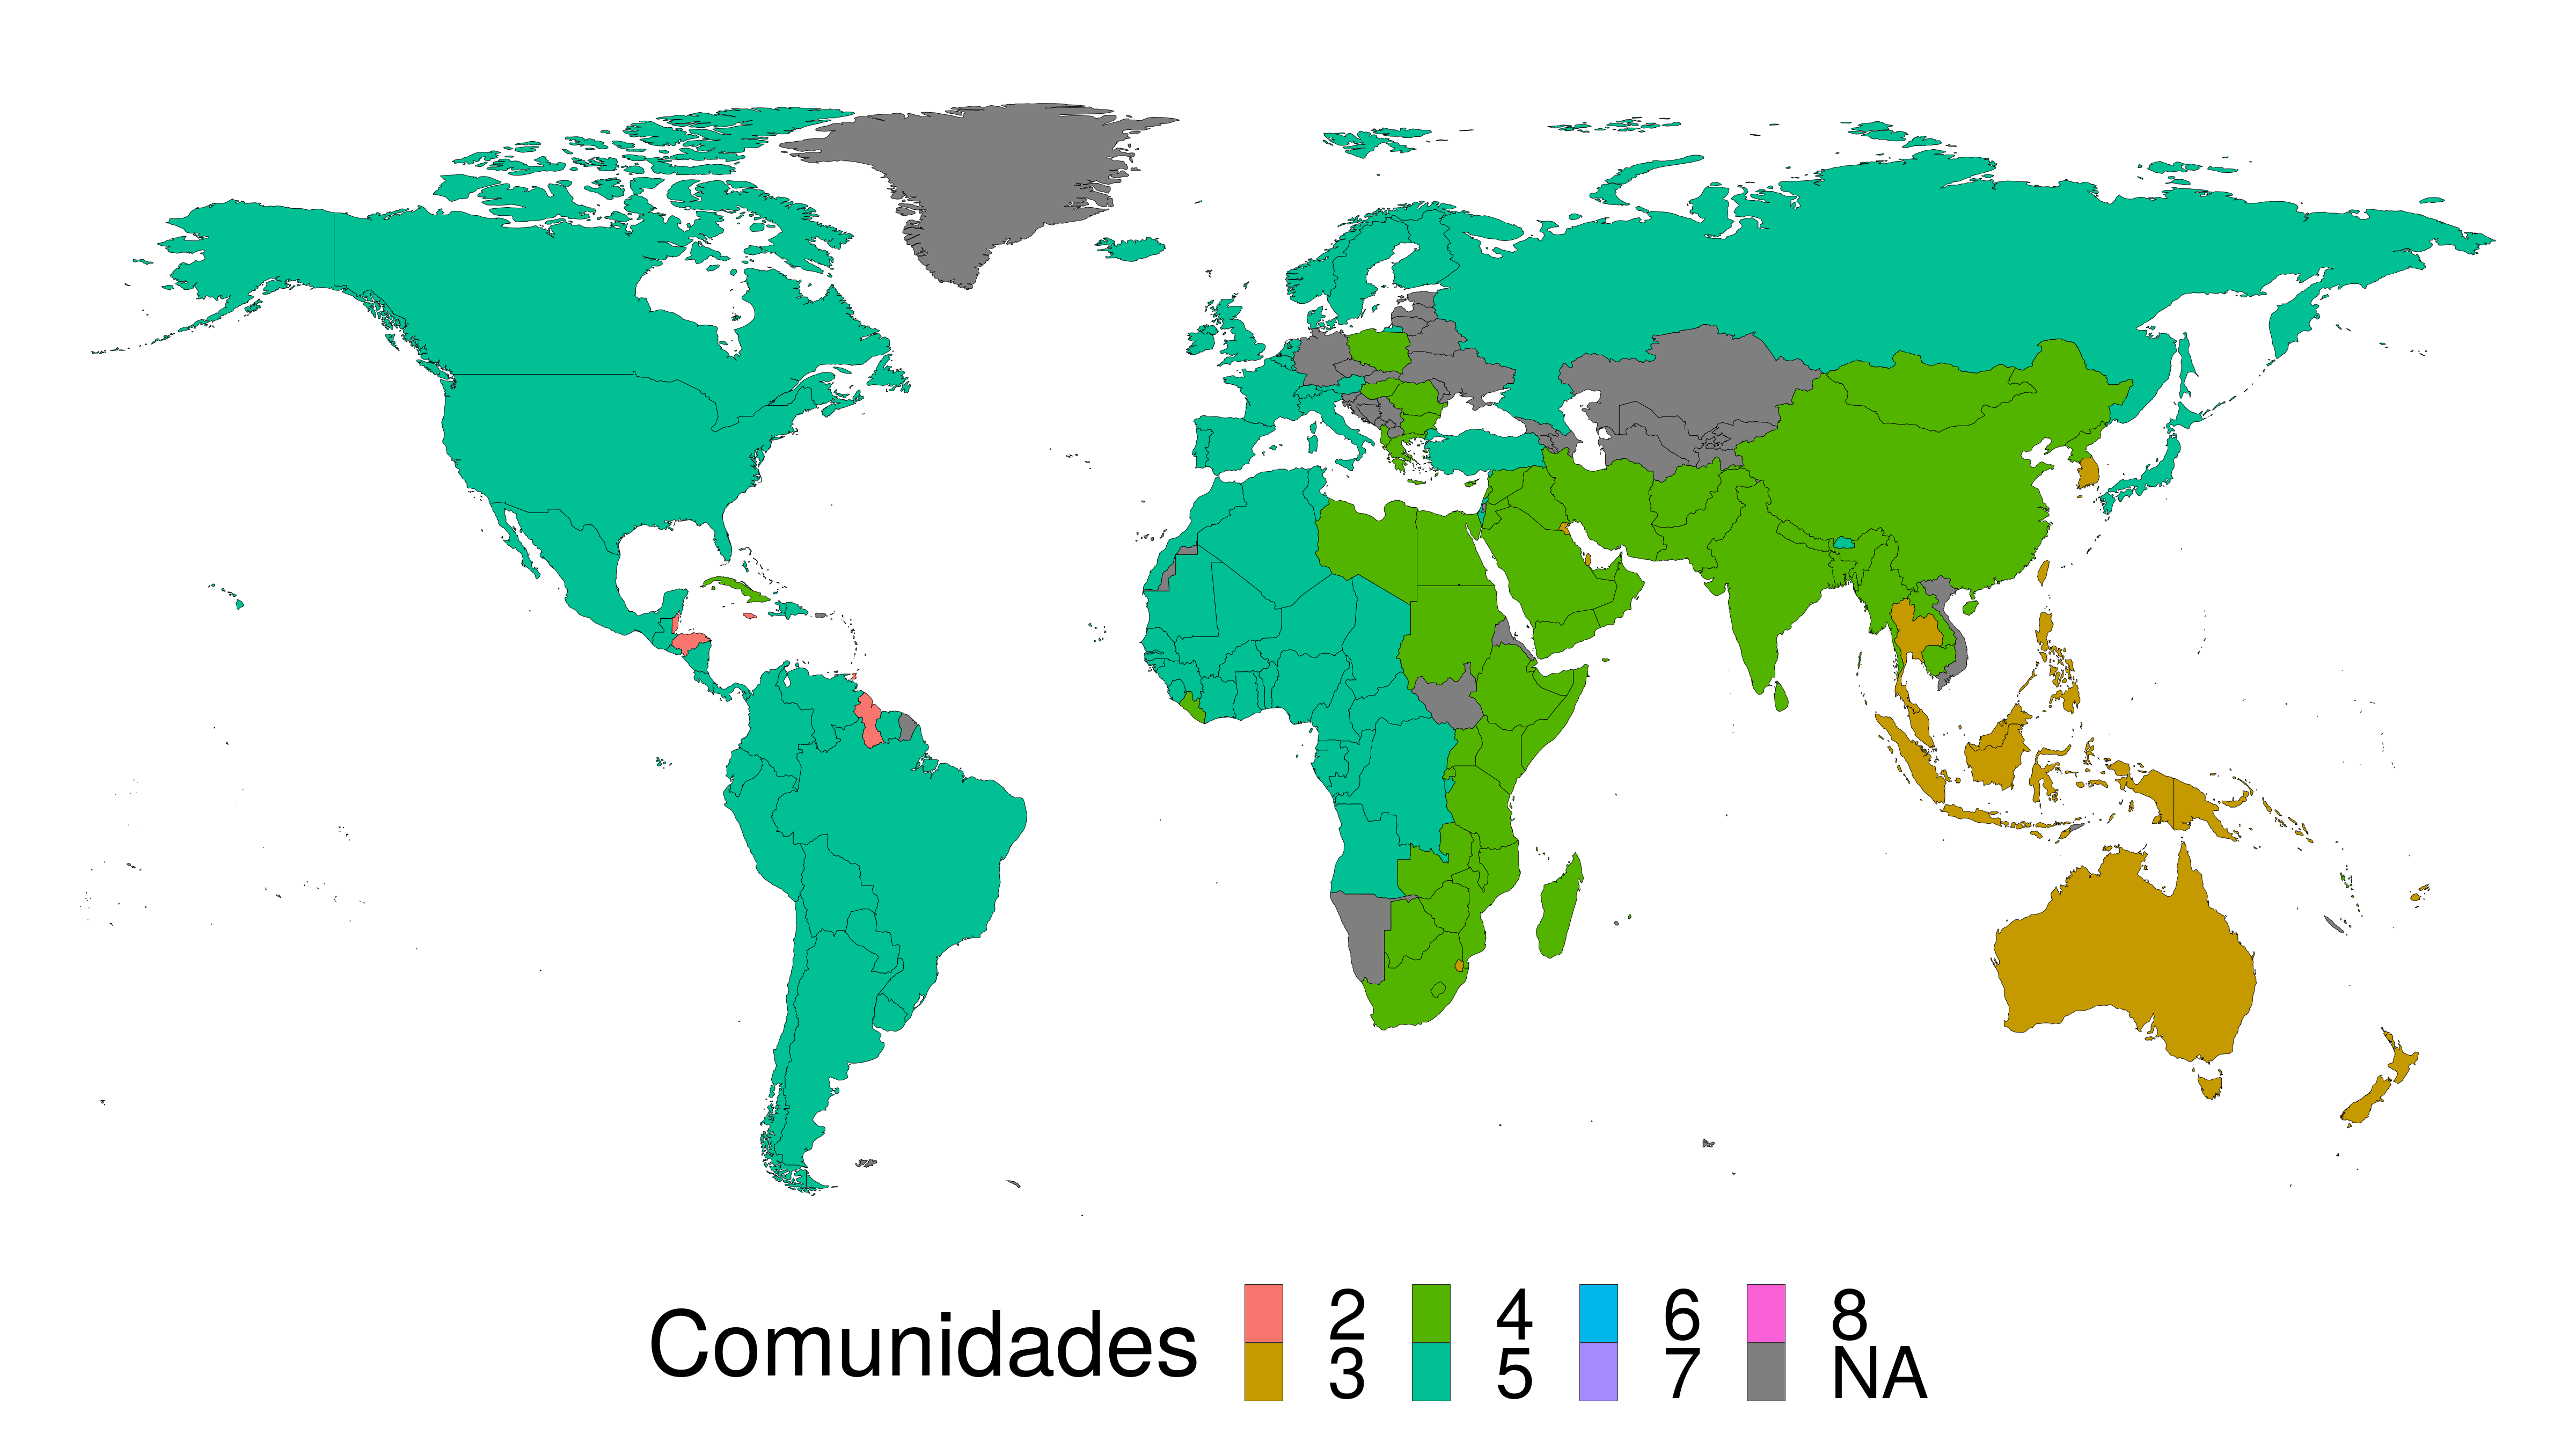
\includegraphics[width=0.45\linewidth]{mapa_walktrap_lp_1986}}
	\subfigure[1996]{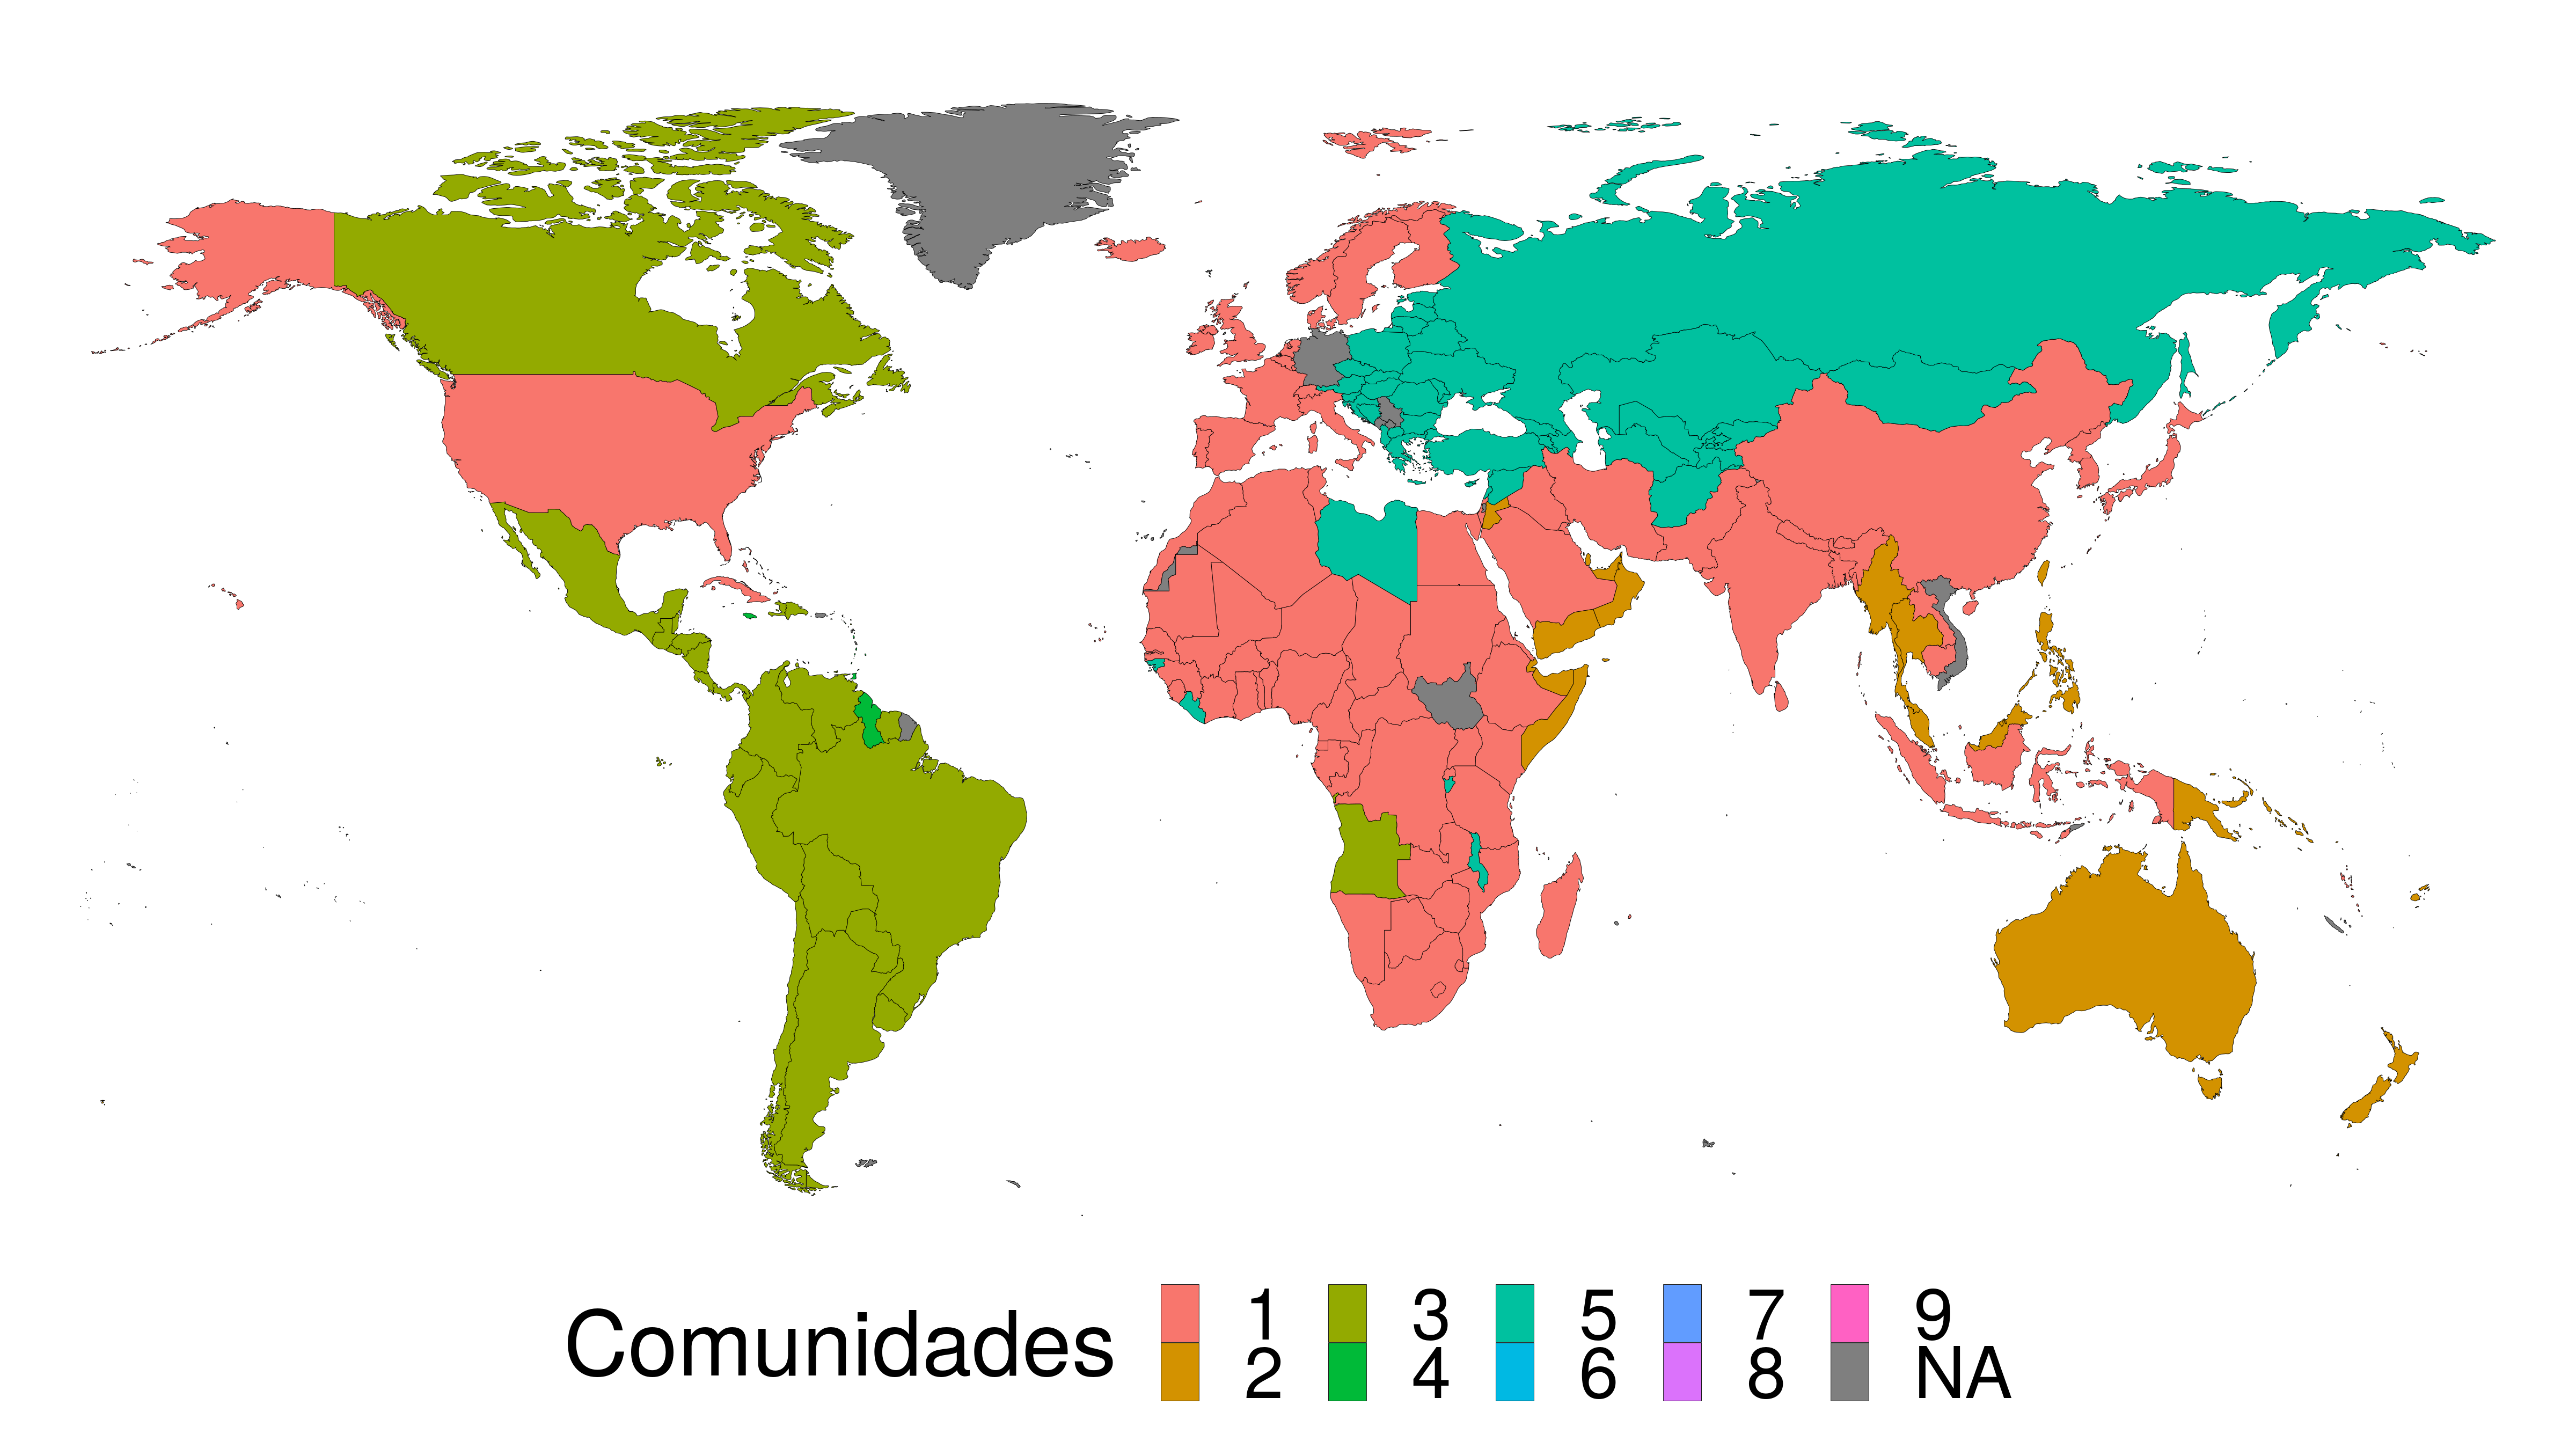
\includegraphics[width=0.45\linewidth]{mapa_walktrap_lp_1996}}
	\subfigure[2016]{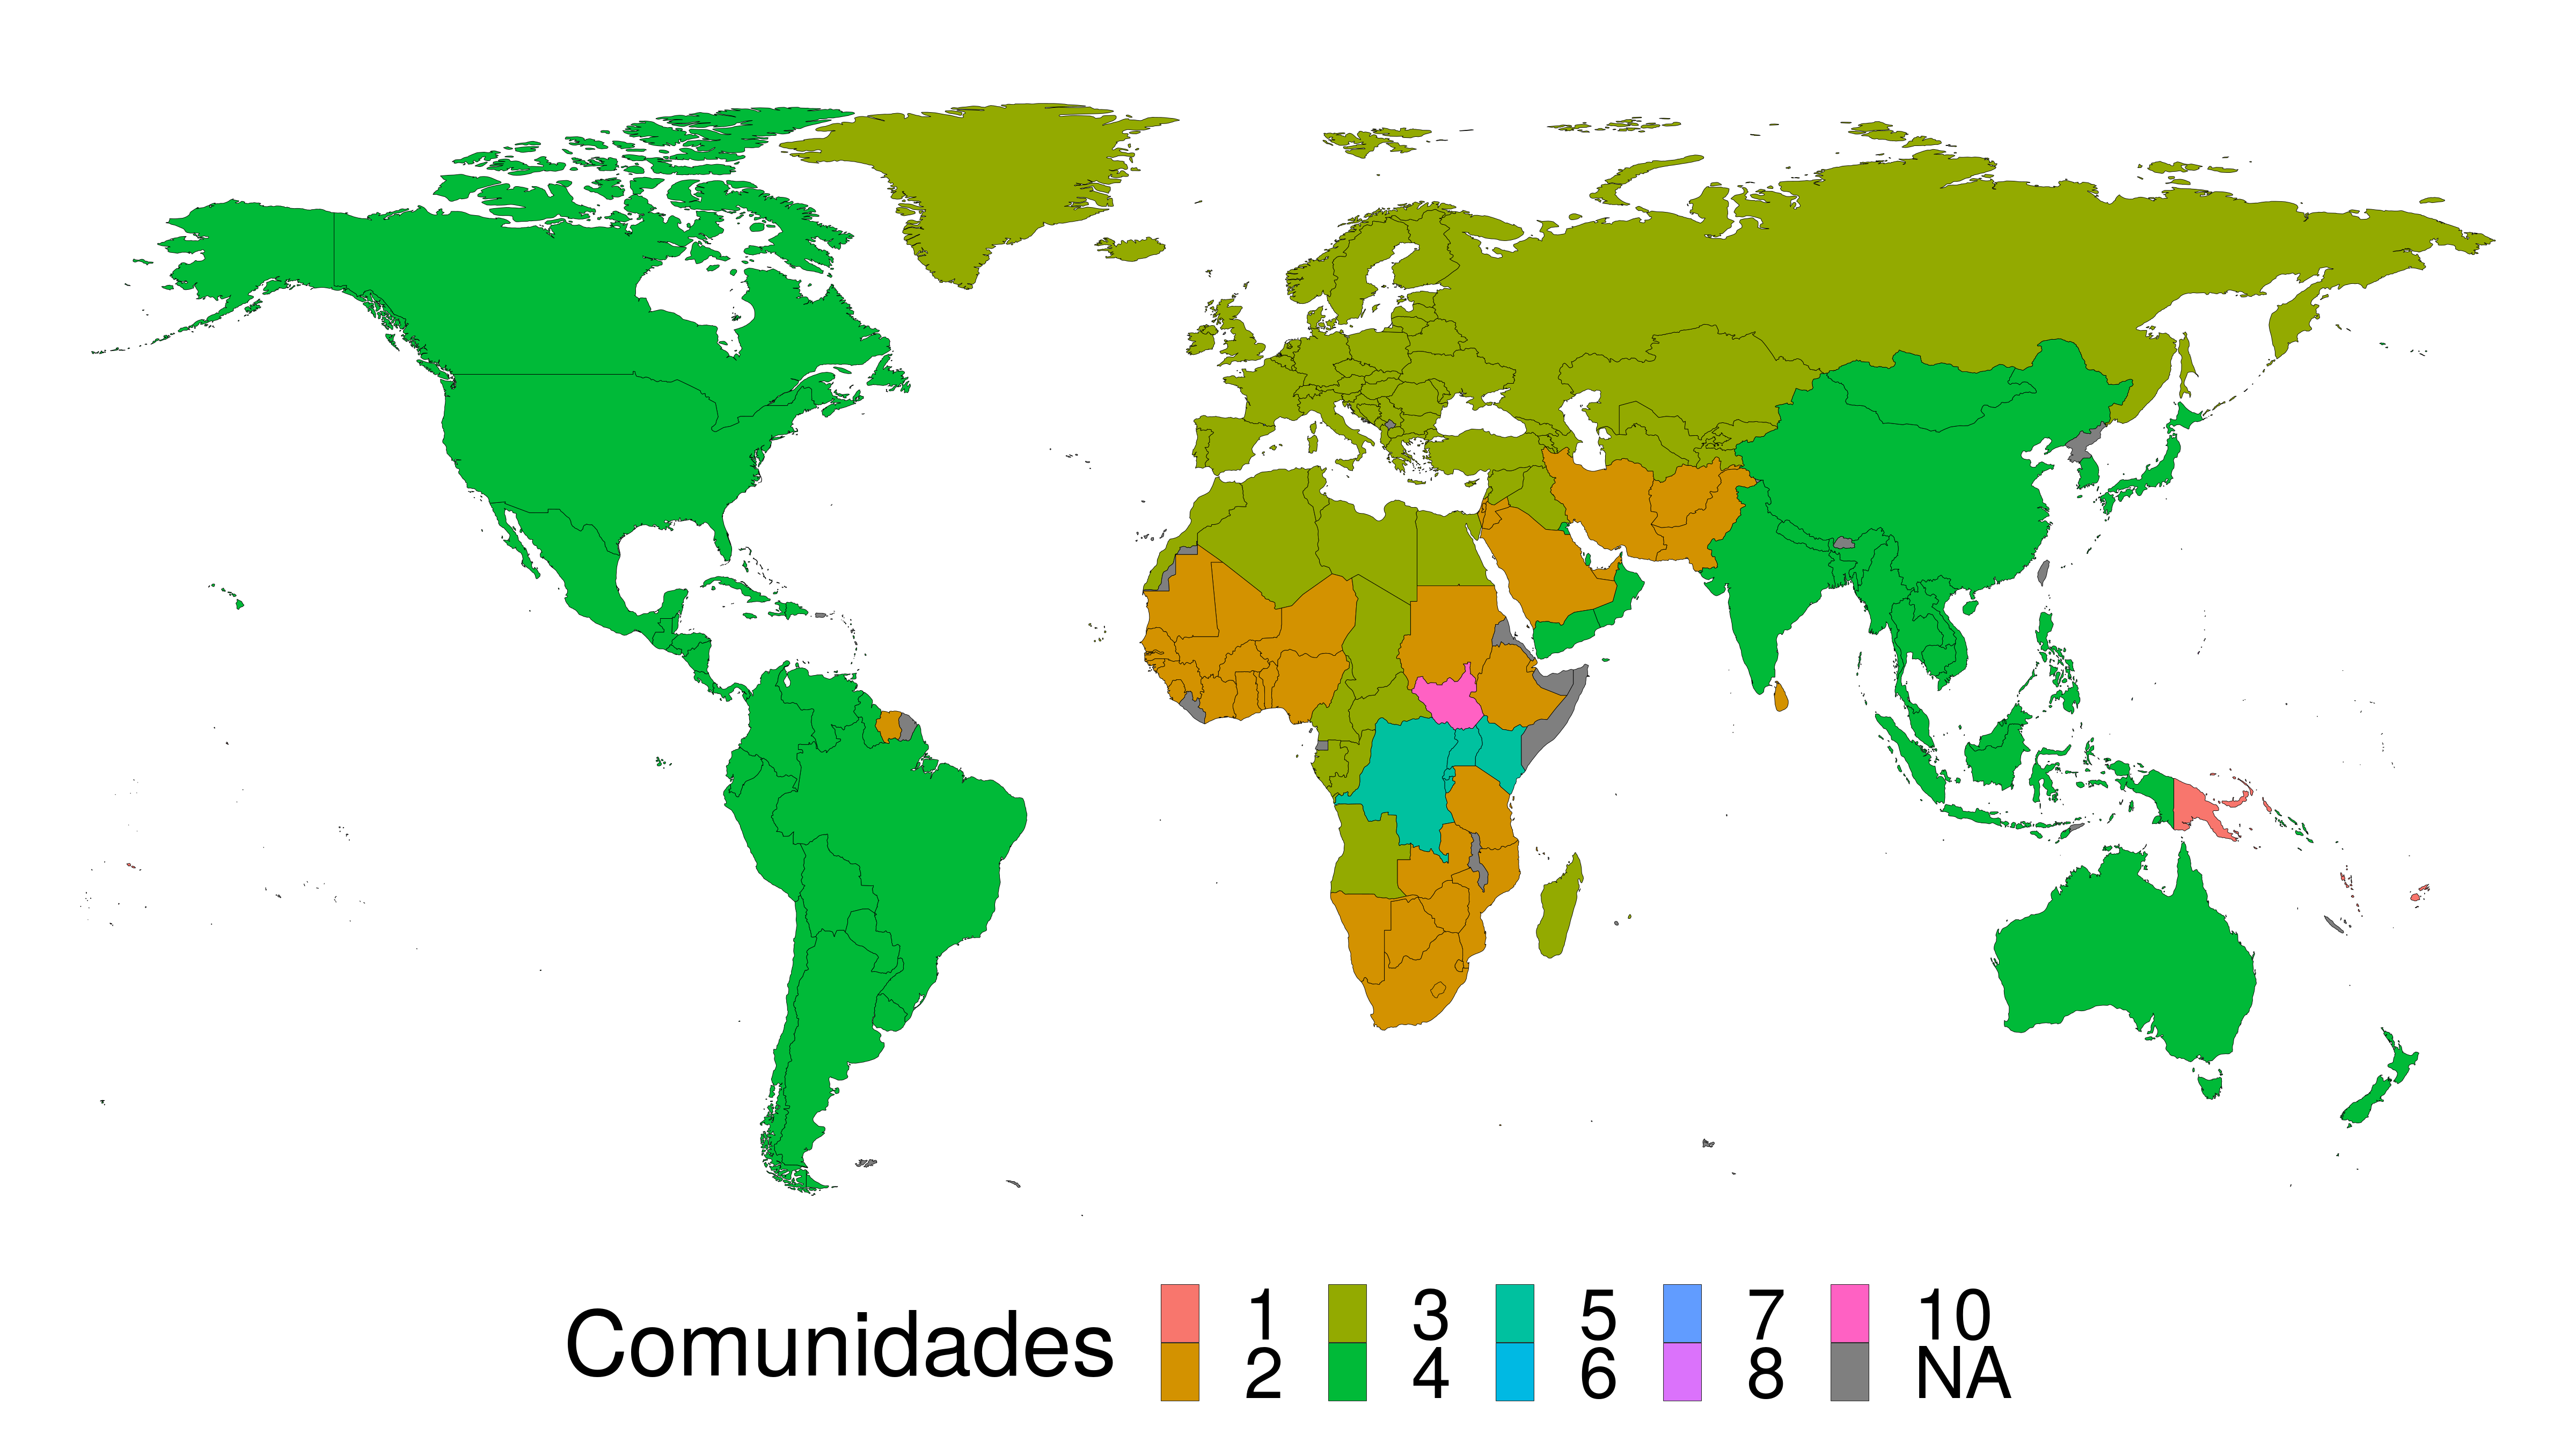
\includegraphics[width=0.45\linewidth]{mapa_walktrap_2016}}
	\caption{Grafo a nivel países. Clustering walktrap. Exportaciones}
	\label{fig:mapas_comercio_walktrap}
\end{figure}

\end{document}